
% Default to the notebook output style

    


% Inherit from the specified cell style.




    
\documentclass[11pt]{article}

    
    
    \usepackage[T1]{fontenc}
    % Nicer default font (+ math font) than Computer Modern for most use cases
    \usepackage{mathpazo}

    % Basic figure setup, for now with no caption control since it's done
    % automatically by Pandoc (which extracts ![](path) syntax from Markdown).
    \usepackage{graphicx}
    % We will generate all images so they have a width \maxwidth. This means
    % that they will get their normal width if they fit onto the page, but
    % are scaled down if they would overflow the margins.
    \makeatletter
    \def\maxwidth{\ifdim\Gin@nat@width>\linewidth\linewidth
    \else\Gin@nat@width\fi}
    \makeatother
    \let\Oldincludegraphics\includegraphics
    % Set max figure width to be 80% of text width, for now hardcoded.
    \renewcommand{\includegraphics}[1]{\Oldincludegraphics[width=.8\maxwidth]{#1}}
    % Ensure that by default, figures have no caption (until we provide a
    % proper Figure object with a Caption API and a way to capture that
    % in the conversion process - todo).
    \usepackage{caption}
    \DeclareCaptionLabelFormat{nolabel}{}
    \captionsetup{labelformat=nolabel}

    \usepackage{adjustbox} % Used to constrain images to a maximum size 
    \usepackage{xcolor} % Allow colors to be defined
    \usepackage{enumerate} % Needed for markdown enumerations to work
    \usepackage{geometry} % Used to adjust the document margins
    \usepackage{amsmath} % Equations
    \usepackage{amssymb} % Equations
    \usepackage{textcomp} % defines textquotesingle
    % Hack from http://tex.stackexchange.com/a/47451/13684:
    \AtBeginDocument{%
        \def\PYZsq{\textquotesingle}% Upright quotes in Pygmentized code
    }
    \usepackage{upquote} % Upright quotes for verbatim code
    \usepackage{eurosym} % defines \euro
    \usepackage[mathletters]{ucs} % Extended unicode (utf-8) support
    \usepackage[utf8x]{inputenc} % Allow utf-8 characters in the tex document
    \usepackage{fancyvrb} % verbatim replacement that allows latex
    \usepackage{grffile} % extends the file name processing of package graphics 
                         % to support a larger range 
    % The hyperref package gives us a pdf with properly built
    % internal navigation ('pdf bookmarks' for the table of contents,
    % internal cross-reference links, web links for URLs, etc.)
    \usepackage{hyperref}
    \usepackage{longtable} % longtable support required by pandoc >1.10
    \usepackage{booktabs}  % table support for pandoc > 1.12.2
    \usepackage[inline]{enumitem} % IRkernel/repr support (it uses the enumerate* environment)
    \usepackage[normalem]{ulem} % ulem is needed to support strikethroughs (\sout)
                                % normalem makes italics be italics, not underlines
    

    
    
    % Colors for the hyperref package
    \definecolor{urlcolor}{rgb}{0,.145,.698}
    \definecolor{linkcolor}{rgb}{.71,0.21,0.01}
    \definecolor{citecolor}{rgb}{.12,.54,.11}

    % ANSI colors
    \definecolor{ansi-black}{HTML}{3E424D}
    \definecolor{ansi-black-intense}{HTML}{282C36}
    \definecolor{ansi-red}{HTML}{E75C58}
    \definecolor{ansi-red-intense}{HTML}{B22B31}
    \definecolor{ansi-green}{HTML}{00A250}
    \definecolor{ansi-green-intense}{HTML}{007427}
    \definecolor{ansi-yellow}{HTML}{DDB62B}
    \definecolor{ansi-yellow-intense}{HTML}{B27D12}
    \definecolor{ansi-blue}{HTML}{208FFB}
    \definecolor{ansi-blue-intense}{HTML}{0065CA}
    \definecolor{ansi-magenta}{HTML}{D160C4}
    \definecolor{ansi-magenta-intense}{HTML}{A03196}
    \definecolor{ansi-cyan}{HTML}{60C6C8}
    \definecolor{ansi-cyan-intense}{HTML}{258F8F}
    \definecolor{ansi-white}{HTML}{C5C1B4}
    \definecolor{ansi-white-intense}{HTML}{A1A6B2}

    % commands and environments needed by pandoc snippets
    % extracted from the output of `pandoc -s`
    \providecommand{\tightlist}{%
      \setlength{\itemsep}{0pt}\setlength{\parskip}{0pt}}
    \DefineVerbatimEnvironment{Highlighting}{Verbatim}{commandchars=\\\{\}}
    % Add ',fontsize=\small' for more characters per line
    \newenvironment{Shaded}{}{}
    \newcommand{\KeywordTok}[1]{\textcolor[rgb]{0.00,0.44,0.13}{\textbf{{#1}}}}
    \newcommand{\DataTypeTok}[1]{\textcolor[rgb]{0.56,0.13,0.00}{{#1}}}
    \newcommand{\DecValTok}[1]{\textcolor[rgb]{0.25,0.63,0.44}{{#1}}}
    \newcommand{\BaseNTok}[1]{\textcolor[rgb]{0.25,0.63,0.44}{{#1}}}
    \newcommand{\FloatTok}[1]{\textcolor[rgb]{0.25,0.63,0.44}{{#1}}}
    \newcommand{\CharTok}[1]{\textcolor[rgb]{0.25,0.44,0.63}{{#1}}}
    \newcommand{\StringTok}[1]{\textcolor[rgb]{0.25,0.44,0.63}{{#1}}}
    \newcommand{\CommentTok}[1]{\textcolor[rgb]{0.38,0.63,0.69}{\textit{{#1}}}}
    \newcommand{\OtherTok}[1]{\textcolor[rgb]{0.00,0.44,0.13}{{#1}}}
    \newcommand{\AlertTok}[1]{\textcolor[rgb]{1.00,0.00,0.00}{\textbf{{#1}}}}
    \newcommand{\FunctionTok}[1]{\textcolor[rgb]{0.02,0.16,0.49}{{#1}}}
    \newcommand{\RegionMarkerTok}[1]{{#1}}
    \newcommand{\ErrorTok}[1]{\textcolor[rgb]{1.00,0.00,0.00}{\textbf{{#1}}}}
    \newcommand{\NormalTok}[1]{{#1}}
    
    % Additional commands for more recent versions of Pandoc
    \newcommand{\ConstantTok}[1]{\textcolor[rgb]{0.53,0.00,0.00}{{#1}}}
    \newcommand{\SpecialCharTok}[1]{\textcolor[rgb]{0.25,0.44,0.63}{{#1}}}
    \newcommand{\VerbatimStringTok}[1]{\textcolor[rgb]{0.25,0.44,0.63}{{#1}}}
    \newcommand{\SpecialStringTok}[1]{\textcolor[rgb]{0.73,0.40,0.53}{{#1}}}
    \newcommand{\ImportTok}[1]{{#1}}
    \newcommand{\DocumentationTok}[1]{\textcolor[rgb]{0.73,0.13,0.13}{\textit{{#1}}}}
    \newcommand{\AnnotationTok}[1]{\textcolor[rgb]{0.38,0.63,0.69}{\textbf{\textit{{#1}}}}}
    \newcommand{\CommentVarTok}[1]{\textcolor[rgb]{0.38,0.63,0.69}{\textbf{\textit{{#1}}}}}
    \newcommand{\VariableTok}[1]{\textcolor[rgb]{0.10,0.09,0.49}{{#1}}}
    \newcommand{\ControlFlowTok}[1]{\textcolor[rgb]{0.00,0.44,0.13}{\textbf{{#1}}}}
    \newcommand{\OperatorTok}[1]{\textcolor[rgb]{0.40,0.40,0.40}{{#1}}}
    \newcommand{\BuiltInTok}[1]{{#1}}
    \newcommand{\ExtensionTok}[1]{{#1}}
    \newcommand{\PreprocessorTok}[1]{\textcolor[rgb]{0.74,0.48,0.00}{{#1}}}
    \newcommand{\AttributeTok}[1]{\textcolor[rgb]{0.49,0.56,0.16}{{#1}}}
    \newcommand{\InformationTok}[1]{\textcolor[rgb]{0.38,0.63,0.69}{\textbf{\textit{{#1}}}}}
    \newcommand{\WarningTok}[1]{\textcolor[rgb]{0.38,0.63,0.69}{\textbf{\textit{{#1}}}}}
    
    
    % Define a nice break command that doesn't care if a line doesn't already
    % exist.
    \def\br{\hspace*{\fill} \\* }
    % Math Jax compatability definitions
    \def\gt{>}
    \def\lt{<}
    % Document parameters
    \title{GAN-1}
    
    
    

    % Pygments definitions
    
\makeatletter
\def\PY@reset{\let\PY@it=\relax \let\PY@bf=\relax%
    \let\PY@ul=\relax \let\PY@tc=\relax%
    \let\PY@bc=\relax \let\PY@ff=\relax}
\def\PY@tok#1{\csname PY@tok@#1\endcsname}
\def\PY@toks#1+{\ifx\relax#1\empty\else%
    \PY@tok{#1}\expandafter\PY@toks\fi}
\def\PY@do#1{\PY@bc{\PY@tc{\PY@ul{%
    \PY@it{\PY@bf{\PY@ff{#1}}}}}}}
\def\PY#1#2{\PY@reset\PY@toks#1+\relax+\PY@do{#2}}

\expandafter\def\csname PY@tok@w\endcsname{\def\PY@tc##1{\textcolor[rgb]{0.73,0.73,0.73}{##1}}}
\expandafter\def\csname PY@tok@c\endcsname{\let\PY@it=\textit\def\PY@tc##1{\textcolor[rgb]{0.25,0.50,0.50}{##1}}}
\expandafter\def\csname PY@tok@cp\endcsname{\def\PY@tc##1{\textcolor[rgb]{0.74,0.48,0.00}{##1}}}
\expandafter\def\csname PY@tok@k\endcsname{\let\PY@bf=\textbf\def\PY@tc##1{\textcolor[rgb]{0.00,0.50,0.00}{##1}}}
\expandafter\def\csname PY@tok@kp\endcsname{\def\PY@tc##1{\textcolor[rgb]{0.00,0.50,0.00}{##1}}}
\expandafter\def\csname PY@tok@kt\endcsname{\def\PY@tc##1{\textcolor[rgb]{0.69,0.00,0.25}{##1}}}
\expandafter\def\csname PY@tok@o\endcsname{\def\PY@tc##1{\textcolor[rgb]{0.40,0.40,0.40}{##1}}}
\expandafter\def\csname PY@tok@ow\endcsname{\let\PY@bf=\textbf\def\PY@tc##1{\textcolor[rgb]{0.67,0.13,1.00}{##1}}}
\expandafter\def\csname PY@tok@nb\endcsname{\def\PY@tc##1{\textcolor[rgb]{0.00,0.50,0.00}{##1}}}
\expandafter\def\csname PY@tok@nf\endcsname{\def\PY@tc##1{\textcolor[rgb]{0.00,0.00,1.00}{##1}}}
\expandafter\def\csname PY@tok@nc\endcsname{\let\PY@bf=\textbf\def\PY@tc##1{\textcolor[rgb]{0.00,0.00,1.00}{##1}}}
\expandafter\def\csname PY@tok@nn\endcsname{\let\PY@bf=\textbf\def\PY@tc##1{\textcolor[rgb]{0.00,0.00,1.00}{##1}}}
\expandafter\def\csname PY@tok@ne\endcsname{\let\PY@bf=\textbf\def\PY@tc##1{\textcolor[rgb]{0.82,0.25,0.23}{##1}}}
\expandafter\def\csname PY@tok@nv\endcsname{\def\PY@tc##1{\textcolor[rgb]{0.10,0.09,0.49}{##1}}}
\expandafter\def\csname PY@tok@no\endcsname{\def\PY@tc##1{\textcolor[rgb]{0.53,0.00,0.00}{##1}}}
\expandafter\def\csname PY@tok@nl\endcsname{\def\PY@tc##1{\textcolor[rgb]{0.63,0.63,0.00}{##1}}}
\expandafter\def\csname PY@tok@ni\endcsname{\let\PY@bf=\textbf\def\PY@tc##1{\textcolor[rgb]{0.60,0.60,0.60}{##1}}}
\expandafter\def\csname PY@tok@na\endcsname{\def\PY@tc##1{\textcolor[rgb]{0.49,0.56,0.16}{##1}}}
\expandafter\def\csname PY@tok@nt\endcsname{\let\PY@bf=\textbf\def\PY@tc##1{\textcolor[rgb]{0.00,0.50,0.00}{##1}}}
\expandafter\def\csname PY@tok@nd\endcsname{\def\PY@tc##1{\textcolor[rgb]{0.67,0.13,1.00}{##1}}}
\expandafter\def\csname PY@tok@s\endcsname{\def\PY@tc##1{\textcolor[rgb]{0.73,0.13,0.13}{##1}}}
\expandafter\def\csname PY@tok@sd\endcsname{\let\PY@it=\textit\def\PY@tc##1{\textcolor[rgb]{0.73,0.13,0.13}{##1}}}
\expandafter\def\csname PY@tok@si\endcsname{\let\PY@bf=\textbf\def\PY@tc##1{\textcolor[rgb]{0.73,0.40,0.53}{##1}}}
\expandafter\def\csname PY@tok@se\endcsname{\let\PY@bf=\textbf\def\PY@tc##1{\textcolor[rgb]{0.73,0.40,0.13}{##1}}}
\expandafter\def\csname PY@tok@sr\endcsname{\def\PY@tc##1{\textcolor[rgb]{0.73,0.40,0.53}{##1}}}
\expandafter\def\csname PY@tok@ss\endcsname{\def\PY@tc##1{\textcolor[rgb]{0.10,0.09,0.49}{##1}}}
\expandafter\def\csname PY@tok@sx\endcsname{\def\PY@tc##1{\textcolor[rgb]{0.00,0.50,0.00}{##1}}}
\expandafter\def\csname PY@tok@m\endcsname{\def\PY@tc##1{\textcolor[rgb]{0.40,0.40,0.40}{##1}}}
\expandafter\def\csname PY@tok@gh\endcsname{\let\PY@bf=\textbf\def\PY@tc##1{\textcolor[rgb]{0.00,0.00,0.50}{##1}}}
\expandafter\def\csname PY@tok@gu\endcsname{\let\PY@bf=\textbf\def\PY@tc##1{\textcolor[rgb]{0.50,0.00,0.50}{##1}}}
\expandafter\def\csname PY@tok@gd\endcsname{\def\PY@tc##1{\textcolor[rgb]{0.63,0.00,0.00}{##1}}}
\expandafter\def\csname PY@tok@gi\endcsname{\def\PY@tc##1{\textcolor[rgb]{0.00,0.63,0.00}{##1}}}
\expandafter\def\csname PY@tok@gr\endcsname{\def\PY@tc##1{\textcolor[rgb]{1.00,0.00,0.00}{##1}}}
\expandafter\def\csname PY@tok@ge\endcsname{\let\PY@it=\textit}
\expandafter\def\csname PY@tok@gs\endcsname{\let\PY@bf=\textbf}
\expandafter\def\csname PY@tok@gp\endcsname{\let\PY@bf=\textbf\def\PY@tc##1{\textcolor[rgb]{0.00,0.00,0.50}{##1}}}
\expandafter\def\csname PY@tok@go\endcsname{\def\PY@tc##1{\textcolor[rgb]{0.53,0.53,0.53}{##1}}}
\expandafter\def\csname PY@tok@gt\endcsname{\def\PY@tc##1{\textcolor[rgb]{0.00,0.27,0.87}{##1}}}
\expandafter\def\csname PY@tok@err\endcsname{\def\PY@bc##1{\setlength{\fboxsep}{0pt}\fcolorbox[rgb]{1.00,0.00,0.00}{1,1,1}{\strut ##1}}}
\expandafter\def\csname PY@tok@kc\endcsname{\let\PY@bf=\textbf\def\PY@tc##1{\textcolor[rgb]{0.00,0.50,0.00}{##1}}}
\expandafter\def\csname PY@tok@kd\endcsname{\let\PY@bf=\textbf\def\PY@tc##1{\textcolor[rgb]{0.00,0.50,0.00}{##1}}}
\expandafter\def\csname PY@tok@kn\endcsname{\let\PY@bf=\textbf\def\PY@tc##1{\textcolor[rgb]{0.00,0.50,0.00}{##1}}}
\expandafter\def\csname PY@tok@kr\endcsname{\let\PY@bf=\textbf\def\PY@tc##1{\textcolor[rgb]{0.00,0.50,0.00}{##1}}}
\expandafter\def\csname PY@tok@bp\endcsname{\def\PY@tc##1{\textcolor[rgb]{0.00,0.50,0.00}{##1}}}
\expandafter\def\csname PY@tok@fm\endcsname{\def\PY@tc##1{\textcolor[rgb]{0.00,0.00,1.00}{##1}}}
\expandafter\def\csname PY@tok@vc\endcsname{\def\PY@tc##1{\textcolor[rgb]{0.10,0.09,0.49}{##1}}}
\expandafter\def\csname PY@tok@vg\endcsname{\def\PY@tc##1{\textcolor[rgb]{0.10,0.09,0.49}{##1}}}
\expandafter\def\csname PY@tok@vi\endcsname{\def\PY@tc##1{\textcolor[rgb]{0.10,0.09,0.49}{##1}}}
\expandafter\def\csname PY@tok@vm\endcsname{\def\PY@tc##1{\textcolor[rgb]{0.10,0.09,0.49}{##1}}}
\expandafter\def\csname PY@tok@sa\endcsname{\def\PY@tc##1{\textcolor[rgb]{0.73,0.13,0.13}{##1}}}
\expandafter\def\csname PY@tok@sb\endcsname{\def\PY@tc##1{\textcolor[rgb]{0.73,0.13,0.13}{##1}}}
\expandafter\def\csname PY@tok@sc\endcsname{\def\PY@tc##1{\textcolor[rgb]{0.73,0.13,0.13}{##1}}}
\expandafter\def\csname PY@tok@dl\endcsname{\def\PY@tc##1{\textcolor[rgb]{0.73,0.13,0.13}{##1}}}
\expandafter\def\csname PY@tok@s2\endcsname{\def\PY@tc##1{\textcolor[rgb]{0.73,0.13,0.13}{##1}}}
\expandafter\def\csname PY@tok@sh\endcsname{\def\PY@tc##1{\textcolor[rgb]{0.73,0.13,0.13}{##1}}}
\expandafter\def\csname PY@tok@s1\endcsname{\def\PY@tc##1{\textcolor[rgb]{0.73,0.13,0.13}{##1}}}
\expandafter\def\csname PY@tok@mb\endcsname{\def\PY@tc##1{\textcolor[rgb]{0.40,0.40,0.40}{##1}}}
\expandafter\def\csname PY@tok@mf\endcsname{\def\PY@tc##1{\textcolor[rgb]{0.40,0.40,0.40}{##1}}}
\expandafter\def\csname PY@tok@mh\endcsname{\def\PY@tc##1{\textcolor[rgb]{0.40,0.40,0.40}{##1}}}
\expandafter\def\csname PY@tok@mi\endcsname{\def\PY@tc##1{\textcolor[rgb]{0.40,0.40,0.40}{##1}}}
\expandafter\def\csname PY@tok@il\endcsname{\def\PY@tc##1{\textcolor[rgb]{0.40,0.40,0.40}{##1}}}
\expandafter\def\csname PY@tok@mo\endcsname{\def\PY@tc##1{\textcolor[rgb]{0.40,0.40,0.40}{##1}}}
\expandafter\def\csname PY@tok@ch\endcsname{\let\PY@it=\textit\def\PY@tc##1{\textcolor[rgb]{0.25,0.50,0.50}{##1}}}
\expandafter\def\csname PY@tok@cm\endcsname{\let\PY@it=\textit\def\PY@tc##1{\textcolor[rgb]{0.25,0.50,0.50}{##1}}}
\expandafter\def\csname PY@tok@cpf\endcsname{\let\PY@it=\textit\def\PY@tc##1{\textcolor[rgb]{0.25,0.50,0.50}{##1}}}
\expandafter\def\csname PY@tok@c1\endcsname{\let\PY@it=\textit\def\PY@tc##1{\textcolor[rgb]{0.25,0.50,0.50}{##1}}}
\expandafter\def\csname PY@tok@cs\endcsname{\let\PY@it=\textit\def\PY@tc##1{\textcolor[rgb]{0.25,0.50,0.50}{##1}}}

\def\PYZbs{\char`\\}
\def\PYZus{\char`\_}
\def\PYZob{\char`\{}
\def\PYZcb{\char`\}}
\def\PYZca{\char`\^}
\def\PYZam{\char`\&}
\def\PYZlt{\char`\<}
\def\PYZgt{\char`\>}
\def\PYZsh{\char`\#}
\def\PYZpc{\char`\%}
\def\PYZdl{\char`\$}
\def\PYZhy{\char`\-}
\def\PYZsq{\char`\'}
\def\PYZdq{\char`\"}
\def\PYZti{\char`\~}
% for compatibility with earlier versions
\def\PYZat{@}
\def\PYZlb{[}
\def\PYZrb{]}
\makeatother


    % Exact colors from NB
    \definecolor{incolor}{rgb}{0.0, 0.0, 0.5}
    \definecolor{outcolor}{rgb}{0.545, 0.0, 0.0}



    
    % Prevent overflowing lines due to hard-to-break entities
    \sloppy 
    % Setup hyperref package
    \hypersetup{
      breaklinks=true,  % so long urls are correctly broken across lines
      colorlinks=true,
      urlcolor=urlcolor,
      linkcolor=linkcolor,
      citecolor=citecolor,
      }
    % Slightly bigger margins than the latex defaults
    
    \geometry{verbose,tmargin=1in,bmargin=1in,lmargin=1in,rmargin=1in}
    
    

    \begin{document}
    
    
    \maketitle
    
    

    
    \hypertarget{week9-gan}{%
\section{Week9: GAN}\label{week9-gan}}

    \hypertarget{ux5b9eux9a8cux8981ux6c42ux4e0eux57faux672cux6d41ux7a0b}{%
\subsection{实验要求与基本流程}\label{ux5b9eux9a8cux8981ux6c42ux4e0eux57faux672cux6d41ux7a0b}}

\hypertarget{ux5b9eux9a8cux8981ux6c42}{%
\subsubsection{实验要求}\label{ux5b9eux9a8cux8981ux6c42}}

\begin{enumerate}
\def\labelenumi{\arabic{enumi}.}
\tightlist
\item
  结合理论课内容,深入理解GAN(Generative Adversarial
  Networks,生成对抗网络)的原理与训练过程.了解GAN网络结构的演变过程与几个基本的GAN的原理(如DCGAN,wGAN等.)
\item
  阅读实验指导书的实验内容,按照提示运行以及补充实验代码,或者简要回答问题.提交作业时,保留实验结果.
\end{enumerate}

\hypertarget{ux5b9eux9a8cux6d41ux7a0b}{%
\subsubsection{实验流程}\label{ux5b9eux9a8cux6d41ux7a0b}}

\begin{itemize}
\tightlist
\item
  GAN的网络结构与训练
\item
  DCGAN
\item
  LSGAN
\item
  WGAN
\item
  WGAN-GP
\end{itemize}

    \hypertarget{gangenerative-adversarial-networks}{%
\subsection{GAN(Generative Adversarial
Networks)}\label{gangenerative-adversarial-networks}}

让我们先来看一个只是用线性层的生成对抗网络(GAN),来简单了解一下GAN的基本网络结构与训练过程.

这个GAN网络结构分为两部分,生成器网络Generator和判别器网络Discriminator.
-
生成器Generator将随机生成的噪声z通过多个线性层生成图片,注意生成器的最后一层是Tanh,所以我们生成的图片的取值范围为{[}-1,1{]},同理,我们会将真实图片归一化(normalize)到{[}-1,1{]}.
-
而判别器Discriminator是一个二分类器,通过多个线性层得到一个概率值来判别图片是``真实''或者是``生成''的,所以在Discriminator的最后是一个sigmoid,来得到图片是``真实''的概率.

在所有的网络结构中我们都使用了LeakyReLU作为激活函数,除了G与D的最后一层,同时,我们在层与层之间我们还加入了BatchNormalization.

    \begin{Verbatim}[commandchars=\\\{\}]
{\color{incolor}In [{\color{incolor}3}]:} \PY{k+kn}{import} \PY{n+nn}{torch}
        \PY{k+kn}{import} \PY{n+nn}{numpy} \PY{k}{as} \PY{n+nn}{np}
        \PY{k+kn}{import} \PY{n+nn}{torch}\PY{n+nn}{.}\PY{n+nn}{nn} \PY{k}{as} \PY{n+nn}{nn}
        \PY{k+kn}{import} \PY{n+nn}{torch}\PY{n+nn}{.}\PY{n+nn}{optim} \PY{k}{as} \PY{n+nn}{optim}
        \PY{k+kn}{import} \PY{n+nn}{torchvision}
        \PY{k+kn}{import} \PY{n+nn}{torchvision}\PY{n+nn}{.}\PY{n+nn}{transforms} \PY{k}{as} \PY{n+nn}{transforms}
        \PY{k+kn}{import} \PY{n+nn}{matplotlib}\PY{n+nn}{.}\PY{n+nn}{pyplot} \PY{k}{as} \PY{n+nn}{plt}
        \PY{o}{\PYZpc{}}\PY{k}{matplotlib} inline
\end{Verbatim}


    \begin{Verbatim}[commandchars=\\\{\}]
{\color{incolor}In [{\color{incolor}4}]:} \PY{k}{class} \PY{n+nc}{Generator}\PY{p}{(}\PY{n}{nn}\PY{o}{.}\PY{n}{Module}\PY{p}{)}\PY{p}{:}
            \PY{k}{def} \PY{n+nf}{\PYZus{}\PYZus{}init\PYZus{}\PYZus{}}\PY{p}{(}\PY{n+nb+bp}{self}\PY{p}{,} \PY{n}{image\PYZus{}size}\PY{o}{=}\PY{l+m+mi}{32}\PY{p}{,} \PY{n}{latent\PYZus{}dim}\PY{o}{=}\PY{l+m+mi}{100}\PY{p}{,} \PY{n}{output\PYZus{}channel}\PY{o}{=}\PY{l+m+mi}{1}\PY{p}{)}\PY{p}{:}
                \PY{l+s+sd}{\PYZdq{}\PYZdq{}\PYZdq{}}
        \PY{l+s+sd}{        image\PYZus{}size: image with and height}
        \PY{l+s+sd}{        latent dim: the dimension of random noise z}
        \PY{l+s+sd}{        output\PYZus{}channel: the channel of generated image, for example, 1 for gray image, 3 for RGB image}
        \PY{l+s+sd}{        \PYZdq{}\PYZdq{}\PYZdq{}}
                \PY{n+nb}{super}\PY{p}{(}\PY{n}{Generator}\PY{p}{,} \PY{n+nb+bp}{self}\PY{p}{)}\PY{o}{.}\PY{n+nf+fm}{\PYZus{}\PYZus{}init\PYZus{}\PYZus{}}\PY{p}{(}\PY{p}{)}
                \PY{n+nb+bp}{self}\PY{o}{.}\PY{n}{latent\PYZus{}dim} \PY{o}{=} \PY{n}{latent\PYZus{}dim}
                \PY{n+nb+bp}{self}\PY{o}{.}\PY{n}{output\PYZus{}channel} \PY{o}{=} \PY{n}{output\PYZus{}channel}
                \PY{n+nb+bp}{self}\PY{o}{.}\PY{n}{image\PYZus{}size} \PY{o}{=} \PY{n}{image\PYZus{}size}
                
                \PY{c+c1}{\PYZsh{} Linear layer: latent\PYZus{}dim \PYZhy{}\PYZgt{} 128 \PYZhy{}\PYZgt{} 256 \PYZhy{}\PYZgt{} 512 \PYZhy{}\PYZgt{} 1024 \PYZhy{}\PYZgt{} output\PYZus{}channel * image\PYZus{}size * image\PYZus{}size \PYZhy{}\PYZgt{} Tanh}
                \PY{n+nb+bp}{self}\PY{o}{.}\PY{n}{model} \PY{o}{=} \PY{n}{nn}\PY{o}{.}\PY{n}{Sequential}\PY{p}{(}
                    \PY{n}{nn}\PY{o}{.}\PY{n}{Linear}\PY{p}{(}\PY{n}{latent\PYZus{}dim}\PY{p}{,} \PY{l+m+mi}{128}\PY{p}{)}\PY{p}{,}
                    \PY{n}{nn}\PY{o}{.}\PY{n}{BatchNorm1d}\PY{p}{(}\PY{l+m+mi}{128}\PY{p}{)}\PY{p}{,}
                    \PY{n}{nn}\PY{o}{.}\PY{n}{LeakyReLU}\PY{p}{(}\PY{l+m+mf}{0.2}\PY{p}{,} \PY{n}{inplace}\PY{o}{=}\PY{k+kc}{True}\PY{p}{)}\PY{p}{,}
                    \PY{n}{nn}\PY{o}{.}\PY{n}{Linear}\PY{p}{(}\PY{l+m+mi}{128}\PY{p}{,} \PY{l+m+mi}{256}\PY{p}{)}\PY{p}{,}
                    \PY{n}{nn}\PY{o}{.}\PY{n}{BatchNorm1d}\PY{p}{(}\PY{l+m+mi}{256}\PY{p}{)}\PY{p}{,}
                    \PY{n}{nn}\PY{o}{.}\PY{n}{LeakyReLU}\PY{p}{(}\PY{l+m+mf}{0.2}\PY{p}{,} \PY{n}{inplace}\PY{o}{=}\PY{k+kc}{True}\PY{p}{)}\PY{p}{,}
                    \PY{n}{nn}\PY{o}{.}\PY{n}{Linear}\PY{p}{(}\PY{l+m+mi}{256}\PY{p}{,} \PY{l+m+mi}{512}\PY{p}{)}\PY{p}{,}
                    \PY{n}{nn}\PY{o}{.}\PY{n}{BatchNorm1d}\PY{p}{(}\PY{l+m+mi}{512}\PY{p}{)}\PY{p}{,}
                    \PY{n}{nn}\PY{o}{.}\PY{n}{LeakyReLU}\PY{p}{(}\PY{l+m+mf}{0.2}\PY{p}{,} \PY{n}{inplace}\PY{o}{=}\PY{k+kc}{True}\PY{p}{)}\PY{p}{,}
                    \PY{n}{nn}\PY{o}{.}\PY{n}{Linear}\PY{p}{(}\PY{l+m+mi}{512}\PY{p}{,} \PY{l+m+mi}{1024}\PY{p}{)}\PY{p}{,}
                    \PY{n}{nn}\PY{o}{.}\PY{n}{BatchNorm1d}\PY{p}{(}\PY{l+m+mi}{1024}\PY{p}{)}\PY{p}{,}
                    \PY{n}{nn}\PY{o}{.}\PY{n}{LeakyReLU}\PY{p}{(}\PY{l+m+mf}{0.2}\PY{p}{,} \PY{n}{inplace}\PY{o}{=}\PY{k+kc}{True}\PY{p}{)}\PY{p}{,}
                    
                    \PY{n}{nn}\PY{o}{.}\PY{n}{Linear}\PY{p}{(}\PY{l+m+mi}{1024}\PY{p}{,} \PY{n}{output\PYZus{}channel} \PY{o}{*} \PY{n}{image\PYZus{}size} \PY{o}{*} \PY{n}{image\PYZus{}size}\PY{p}{)}\PY{p}{,}
                    \PY{n}{nn}\PY{o}{.}\PY{n}{Tanh}\PY{p}{(}\PY{p}{)}
                \PY{p}{)}
        
            \PY{k}{def} \PY{n+nf}{forward}\PY{p}{(}\PY{n+nb+bp}{self}\PY{p}{,} \PY{n}{z}\PY{p}{)}\PY{p}{:}
                \PY{n}{img} \PY{o}{=} \PY{n+nb+bp}{self}\PY{o}{.}\PY{n}{model}\PY{p}{(}\PY{n}{z}\PY{p}{)}
                \PY{n}{img} \PY{o}{=} \PY{n}{img}\PY{o}{.}\PY{n}{view}\PY{p}{(}\PY{n}{img}\PY{o}{.}\PY{n}{size}\PY{p}{(}\PY{l+m+mi}{0}\PY{p}{)}\PY{p}{,} \PY{n+nb+bp}{self}\PY{o}{.}\PY{n}{output\PYZus{}channel}\PY{p}{,} \PY{n+nb+bp}{self}\PY{o}{.}\PY{n}{image\PYZus{}size}\PY{p}{,} \PY{n+nb+bp}{self}\PY{o}{.}\PY{n}{image\PYZus{}size}\PY{p}{)}
                \PY{k}{return} \PY{n}{img}
        
        
        \PY{k}{class} \PY{n+nc}{Discriminator}\PY{p}{(}\PY{n}{nn}\PY{o}{.}\PY{n}{Module}\PY{p}{)}\PY{p}{:}
            \PY{k}{def} \PY{n+nf}{\PYZus{}\PYZus{}init\PYZus{}\PYZus{}}\PY{p}{(}\PY{n+nb+bp}{self}\PY{p}{,} \PY{n}{image\PYZus{}size}\PY{o}{=}\PY{l+m+mi}{32}\PY{p}{,} \PY{n}{input\PYZus{}channel}\PY{o}{=}\PY{l+m+mi}{1}\PY{p}{)}\PY{p}{:}
                \PY{l+s+sd}{\PYZdq{}\PYZdq{}\PYZdq{}}
        \PY{l+s+sd}{        image\PYZus{}size: image with and height}
        \PY{l+s+sd}{        input\PYZus{}channel: the channel of input image, for example, 1 for gray image, 3 for RGB image}
        \PY{l+s+sd}{        \PYZdq{}\PYZdq{}\PYZdq{}}
                \PY{n+nb}{super}\PY{p}{(}\PY{n}{Discriminator}\PY{p}{,} \PY{n+nb+bp}{self}\PY{p}{)}\PY{o}{.}\PY{n+nf+fm}{\PYZus{}\PYZus{}init\PYZus{}\PYZus{}}\PY{p}{(}\PY{p}{)}
                \PY{n+nb+bp}{self}\PY{o}{.}\PY{n}{image\PYZus{}size} \PY{o}{=} \PY{n}{image\PYZus{}size}
                \PY{n+nb+bp}{self}\PY{o}{.}\PY{n}{input\PYZus{}channel} \PY{o}{=} \PY{n}{input\PYZus{}channel}
                
                \PY{c+c1}{\PYZsh{} Linear layer: input\PYZus{}channel * image\PYZus{}size * image\PYZus{}size \PYZhy{}\PYZgt{} 1024 \PYZhy{}\PYZgt{} 512 \PYZhy{}\PYZgt{} 256 \PYZhy{}\PYZgt{} 1 \PYZhy{}\PYZgt{} Sigmoid}
                \PY{n+nb+bp}{self}\PY{o}{.}\PY{n}{model} \PY{o}{=} \PY{n}{nn}\PY{o}{.}\PY{n}{Sequential}\PY{p}{(}
                    \PY{n}{nn}\PY{o}{.}\PY{n}{Linear}\PY{p}{(}\PY{n}{input\PYZus{}channel} \PY{o}{*} \PY{n}{image\PYZus{}size} \PY{o}{*} \PY{n}{image\PYZus{}size}\PY{p}{,} \PY{l+m+mi}{1024}\PY{p}{)}\PY{p}{,}
                    \PY{n}{nn}\PY{o}{.}\PY{n}{LeakyReLU}\PY{p}{(}\PY{l+m+mf}{0.2}\PY{p}{,} \PY{n}{inplace}\PY{o}{=}\PY{k+kc}{True}\PY{p}{)}\PY{p}{,}
                    \PY{n}{nn}\PY{o}{.}\PY{n}{Linear}\PY{p}{(}\PY{l+m+mi}{1024}\PY{p}{,} \PY{l+m+mi}{512}\PY{p}{)}\PY{p}{,}
                    \PY{n}{nn}\PY{o}{.}\PY{n}{LeakyReLU}\PY{p}{(}\PY{l+m+mf}{0.2}\PY{p}{,} \PY{n}{inplace}\PY{o}{=}\PY{k+kc}{True}\PY{p}{)}\PY{p}{,}
                    \PY{n}{nn}\PY{o}{.}\PY{n}{Linear}\PY{p}{(}\PY{l+m+mi}{512}\PY{p}{,} \PY{l+m+mi}{256}\PY{p}{)}\PY{p}{,}
                    \PY{n}{nn}\PY{o}{.}\PY{n}{LeakyReLU}\PY{p}{(}\PY{l+m+mf}{0.2}\PY{p}{,} \PY{n}{inplace}\PY{o}{=}\PY{k+kc}{True}\PY{p}{)}\PY{p}{,}
                    \PY{n}{nn}\PY{o}{.}\PY{n}{Linear}\PY{p}{(}\PY{l+m+mi}{256}\PY{p}{,} \PY{l+m+mi}{1}\PY{p}{)}\PY{p}{,}
                    \PY{n}{nn}\PY{o}{.}\PY{n}{Sigmoid}\PY{p}{(}\PY{p}{)}\PY{p}{,}
                \PY{p}{)}
        
            \PY{k}{def} \PY{n+nf}{forward}\PY{p}{(}\PY{n+nb+bp}{self}\PY{p}{,} \PY{n}{img}\PY{p}{)}\PY{p}{:}
                \PY{n}{img\PYZus{}flat} \PY{o}{=} \PY{n}{img}\PY{o}{.}\PY{n}{view}\PY{p}{(}\PY{n}{img}\PY{o}{.}\PY{n}{size}\PY{p}{(}\PY{l+m+mi}{0}\PY{p}{)}\PY{p}{,} \PY{o}{\PYZhy{}}\PY{l+m+mi}{1}\PY{p}{)}
                \PY{n}{out} \PY{o}{=} \PY{n+nb+bp}{self}\PY{o}{.}\PY{n}{model}\PY{p}{(}\PY{n}{img\PYZus{}flat}\PY{p}{)}
                \PY{k}{return} \PY{n}{out}
\end{Verbatim}


    \hypertarget{ux6570ux636eux96c6}{%
\subsubsection{数据集}\label{ux6570ux636eux96c6}}

在训练我们的GAN网络之前,
先介绍一下本次实验可训练GAN的数据集,我们提供了两个数据集来供大家进行尝试数据集.
-
MNIST手写体3类数据集,这里为了加快我们的训练速度,我们提供了一个简化版本的只包含数字0,2的2类MNIST数据集,每类各1000张.图片为28*28的单通道灰度图(我们将其resize到32*32),对于GAN而言,我们不需要测试集.我们本次实验主要使用该数据集作为主要的训练数据集.

\begin{itemize}
\tightlist
\item
  室内家具数据集.为了加快我们的训练速度,我们将其做了删减处理,仅包含chair等一个类,共500张.图片为32*32的3通道彩色图片.
\end{itemize}

下面是两个加载数据集的函数.注意我们将所有图片normalize到了{[}-1,1{]}之间.

    \begin{Verbatim}[commandchars=\\\{\}]
{\color{incolor}In [{\color{incolor}5}]:} \PY{k}{def} \PY{n+nf}{load\PYZus{}mnist\PYZus{}data}\PY{p}{(}\PY{p}{)}\PY{p}{:}
            \PY{l+s+sd}{\PYZdq{}\PYZdq{}\PYZdq{}}
        \PY{l+s+sd}{    load mnist(0,1,2) dataset }
        \PY{l+s+sd}{    \PYZdq{}\PYZdq{}\PYZdq{}}
            
            \PY{n}{transform} \PY{o}{=} \PY{n}{torchvision}\PY{o}{.}\PY{n}{transforms}\PY{o}{.}\PY{n}{Compose}\PY{p}{(}\PY{p}{[}
                \PY{c+c1}{\PYZsh{} transform to 1\PYZhy{}channel gray image since we reading image in RGB mode}
                \PY{n}{transforms}\PY{o}{.}\PY{n}{Grayscale}\PY{p}{(}\PY{l+m+mi}{1}\PY{p}{)}\PY{p}{,}
                \PY{c+c1}{\PYZsh{} resize image from 28 * 28 to 32 * 32}
                \PY{n}{transforms}\PY{o}{.}\PY{n}{Resize}\PY{p}{(}\PY{l+m+mi}{32}\PY{p}{)}\PY{p}{,}
                \PY{n}{transforms}\PY{o}{.}\PY{n}{ToTensor}\PY{p}{(}\PY{p}{)}\PY{p}{,}
                \PY{c+c1}{\PYZsh{} normalize with mean=0.5 std=0.5}
                \PY{n}{transforms}\PY{o}{.}\PY{n}{Normalize}\PY{p}{(}\PY{n}{mean}\PY{o}{=}\PY{p}{(}\PY{l+m+mf}{0.5}\PY{p}{,} \PY{p}{)}\PY{p}{,} 
                                     \PY{n}{std}\PY{o}{=}\PY{p}{(}\PY{l+m+mf}{0.5}\PY{p}{,} \PY{p}{)}\PY{p}{)}
                \PY{p}{]}\PY{p}{)}
            
            \PY{n}{train\PYZus{}dataset} \PY{o}{=} \PY{n}{torchvision}\PY{o}{.}\PY{n}{datasets}\PY{o}{.}\PY{n}{ImageFolder}\PY{p}{(}\PY{n}{root}\PY{o}{=}\PY{l+s+s1}{\PYZsq{}}\PY{l+s+s1}{./data/mnist}\PY{l+s+s1}{\PYZsq{}}\PY{p}{,} \PY{n}{transform}\PY{o}{=}\PY{n}{transform}\PY{p}{)}
            
            \PY{k}{return} \PY{n}{train\PYZus{}dataset}
        
        \PY{k}{def} \PY{n+nf}{load\PYZus{}furniture\PYZus{}data}\PY{p}{(}\PY{p}{)}\PY{p}{:}
            \PY{l+s+sd}{\PYZdq{}\PYZdq{}\PYZdq{}}
        \PY{l+s+sd}{    load furniture dataset }
        \PY{l+s+sd}{    \PYZdq{}\PYZdq{}\PYZdq{}}
            \PY{n}{transform} \PY{o}{=} \PY{n}{torchvision}\PY{o}{.}\PY{n}{transforms}\PY{o}{.}\PY{n}{Compose}\PY{p}{(}\PY{p}{[}
                \PY{n}{transforms}\PY{o}{.}\PY{n}{ToTensor}\PY{p}{(}\PY{p}{)}\PY{p}{,}
                \PY{c+c1}{\PYZsh{} normalize with mean=0.5 std=0.5}
                \PY{n}{transforms}\PY{o}{.}\PY{n}{Normalize}\PY{p}{(}\PY{n}{mean}\PY{o}{=}\PY{p}{(}\PY{l+m+mf}{0.5}\PY{p}{,} \PY{l+m+mf}{0.5}\PY{p}{,} \PY{l+m+mf}{0.5}\PY{p}{)}\PY{p}{,} 
                                     \PY{n}{std}\PY{o}{=}\PY{p}{(}\PY{l+m+mf}{0.5}\PY{p}{,} \PY{l+m+mf}{0.5}\PY{p}{,} \PY{l+m+mf}{0.5}\PY{p}{)}\PY{p}{)}
                \PY{p}{]}\PY{p}{)}
            \PY{n}{train\PYZus{}dataset} \PY{o}{=} \PY{n}{torchvision}\PY{o}{.}\PY{n}{datasets}\PY{o}{.}\PY{n}{ImageFolder}\PY{p}{(}\PY{n}{root}\PY{o}{=}\PY{l+s+s1}{\PYZsq{}}\PY{l+s+s1}{./data/household\PYZus{}furniture}\PY{l+s+s1}{\PYZsq{}}\PY{p}{,} \PY{n}{transform}\PY{o}{=}\PY{n}{transform}\PY{p}{)}
            \PY{k}{return} \PY{n}{train\PYZus{}dataset}
\end{Verbatim}


    (\emph{无需阅读理解})运行下面2个cell的代码来查看两个数据集中的20张随机真实图片.

    \begin{Verbatim}[commandchars=\\\{\}]
{\color{incolor}In [{\color{incolor}6}]:} \PY{k}{def} \PY{n+nf}{denorm}\PY{p}{(}\PY{n}{x}\PY{p}{)}\PY{p}{:}
            \PY{c+c1}{\PYZsh{} denormalize}
            \PY{n}{out} \PY{o}{=} \PY{p}{(}\PY{n}{x} \PY{o}{+} \PY{l+m+mi}{1}\PY{p}{)} \PY{o}{/} \PY{l+m+mi}{2}
            \PY{k}{return} \PY{n}{out}\PY{o}{.}\PY{n}{clamp}\PY{p}{(}\PY{l+m+mi}{0}\PY{p}{,} \PY{l+m+mi}{1}\PY{p}{)}
\end{Verbatim}


    \begin{Verbatim}[commandchars=\\\{\}]
{\color{incolor}In [{\color{incolor}7}]:} \PY{k+kn}{from} \PY{n+nn}{utils} \PY{k}{import} \PY{n}{show}
        \PY{l+s+sd}{\PYZdq{}\PYZdq{}\PYZdq{}}
        \PY{l+s+sd}{you can pass code in this cell}
        \PY{l+s+sd}{\PYZdq{}\PYZdq{}\PYZdq{}}
        \PY{c+c1}{\PYZsh{} show mnist real data}
        \PY{n}{train\PYZus{}dataset} \PY{o}{=} \PY{n}{load\PYZus{}mnist\PYZus{}data}\PY{p}{(}\PY{p}{)}
        \PY{n}{trainloader} \PY{o}{=} \PY{n}{torch}\PY{o}{.}\PY{n}{utils}\PY{o}{.}\PY{n}{data}\PY{o}{.}\PY{n}{DataLoader}\PY{p}{(}\PY{n}{train\PYZus{}dataset}\PY{p}{,} \PY{n}{batch\PYZus{}size}\PY{o}{=}\PY{l+m+mi}{20}\PY{p}{,} \PY{n}{shuffle}\PY{o}{=}\PY{k+kc}{True}\PY{p}{)}
        \PY{n}{show}\PY{p}{(}\PY{n}{torchvision}\PY{o}{.}\PY{n}{utils}\PY{o}{.}\PY{n}{make\PYZus{}grid}\PY{p}{(}\PY{n}{denorm}\PY{p}{(}\PY{n+nb}{next}\PY{p}{(}\PY{n+nb}{iter}\PY{p}{(}\PY{n}{trainloader}\PY{p}{)}\PY{p}{)}\PY{p}{[}\PY{l+m+mi}{0}\PY{p}{]}\PY{p}{)}\PY{p}{,} \PY{n}{nrow}\PY{o}{=}\PY{l+m+mi}{5}\PY{p}{)}\PY{p}{)}
        \PY{c+c1}{\PYZsh{} show furniture real data}
        \PY{n}{train\PYZus{}dataset} \PY{o}{=} \PY{n}{load\PYZus{}furniture\PYZus{}data}\PY{p}{(}\PY{p}{)}
        \PY{n}{trainloader} \PY{o}{=} \PY{n}{torch}\PY{o}{.}\PY{n}{utils}\PY{o}{.}\PY{n}{data}\PY{o}{.}\PY{n}{DataLoader}\PY{p}{(}\PY{n}{train\PYZus{}dataset}\PY{p}{,} \PY{n}{batch\PYZus{}size}\PY{o}{=}\PY{l+m+mi}{20}\PY{p}{,} \PY{n}{shuffle}\PY{o}{=}\PY{k+kc}{True}\PY{p}{)}
        \PY{n}{show}\PY{p}{(}\PY{n}{torchvision}\PY{o}{.}\PY{n}{utils}\PY{o}{.}\PY{n}{make\PYZus{}grid}\PY{p}{(}\PY{n}{denorm}\PY{p}{(}\PY{n+nb}{next}\PY{p}{(}\PY{n+nb}{iter}\PY{p}{(}\PY{n}{trainloader}\PY{p}{)}\PY{p}{)}\PY{p}{[}\PY{l+m+mi}{0}\PY{p}{]}\PY{p}{)}\PY{p}{,} \PY{n}{nrow}\PY{o}{=}\PY{l+m+mi}{5}\PY{p}{)}\PY{p}{)}
\end{Verbatim}


    \begin{center}
    \adjustimage{max size={0.9\linewidth}{0.9\paperheight}}{output_9_0.png}
    \end{center}
    { \hspace*{\fill} \\}
    
    \begin{center}
    \adjustimage{max size={0.9\linewidth}{0.9\paperheight}}{output_9_1.png}
    \end{center}
    { \hspace*{\fill} \\}
    
    下面代码实现GAN在一个epoch内的训练过程.

大体而言,GAN的训练过程分为两步,首先将随机噪声z喂给G,生成图片,然后将真实图片和G生成的图片喂给D,然后使用对应的loss函数反向传播优化D.然后再次使用G生成图片,并喂给D,并使用对应的loss函数反向传播优化G.

下面的图片是普通的GAN在G和D上的优化目标:
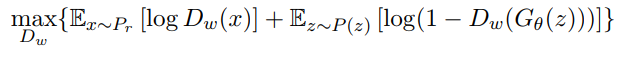
\includegraphics{./pictures/gan_d.png}
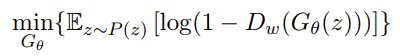
\includegraphics{./pictures/gan_g.png}
值得注意的是,上述图片描述的是G和D的\textbf{优化目标},而在具体实现过程中,我们实现loss函数来达到优化目标.对于上图中D与G的优化目标我们可以使用Binary
Cross Entroy损失函数来实现: \[
BCEloss(p_i,y_i)= -(y_i\log{p_i}+(1−y_i)\log{(1−p_i)})
\] \(p_i\),
\(y_i\)分别是模型的预测值与图片的真实标签(1为真,0为假).因此,对于D,最大化其优化目标可以通过最小化一个BCEloss来实现,其真实图片\(x\sim{P_r}\)的标签设置为1,而生成图片\(z\sim{P(z)}\)的标签设置为0.我们可以看到这样的损失函数相当于对D的优化目标加上负号.

而对于G,也通过最小化一个BCEloss来实现,即将生成图片\(z\sim{P(z)}\)的标签设置为1即可,我们可以看到这样的损失函数与其优化目标是一致的.

    \begin{Verbatim}[commandchars=\\\{\}]
{\color{incolor}In [{\color{incolor}8}]:} \PY{k}{def} \PY{n+nf}{train}\PY{p}{(}\PY{n}{trainloader}\PY{p}{,} \PY{n}{G}\PY{p}{,} \PY{n}{D}\PY{p}{,} \PY{n}{G\PYZus{}optimizer}\PY{p}{,} \PY{n}{D\PYZus{}optimizer}\PY{p}{,} \PY{n}{loss\PYZus{}func}\PY{p}{,} \PY{n}{device}\PY{p}{,} \PY{n}{z\PYZus{}dim}\PY{p}{)}\PY{p}{:}
            \PY{l+s+sd}{\PYZdq{}\PYZdq{}\PYZdq{}}
        \PY{l+s+sd}{    train a GAN with model G and D in one epoch}
        \PY{l+s+sd}{    Args:}
        \PY{l+s+sd}{        trainloader: data loader to train}
        \PY{l+s+sd}{        G: model Generator}
        \PY{l+s+sd}{        D: model Discriminator}
        \PY{l+s+sd}{        G\PYZus{}optimizer: optimizer of G(etc. Adam, SGD)}
        \PY{l+s+sd}{        D\PYZus{}optimizer: optimizer of D(etc. Adam, SGD)}
        \PY{l+s+sd}{        loss\PYZus{}func: loss function to train G and D. For example, Binary Cross Entropy(BCE) loss function}
        \PY{l+s+sd}{        device: cpu or cuda device}
        \PY{l+s+sd}{        z\PYZus{}dim: the dimension of random noise z}
        \PY{l+s+sd}{    \PYZdq{}\PYZdq{}\PYZdq{}}
            \PY{c+c1}{\PYZsh{} set train mode}
            \PY{n}{D}\PY{o}{.}\PY{n}{train}\PY{p}{(}\PY{p}{)}
            \PY{n}{G}\PY{o}{.}\PY{n}{train}\PY{p}{(}\PY{p}{)}
            
            \PY{n}{D\PYZus{}total\PYZus{}loss} \PY{o}{=} \PY{l+m+mi}{0}
            \PY{n}{G\PYZus{}total\PYZus{}loss} \PY{o}{=} \PY{l+m+mi}{0}
            
            
            \PY{k}{for} \PY{n}{i}\PY{p}{,} \PY{p}{(}\PY{n}{x}\PY{p}{,} \PY{n}{\PYZus{}}\PY{p}{)} \PY{o+ow}{in} \PY{n+nb}{enumerate}\PY{p}{(}\PY{n}{trainloader}\PY{p}{)}\PY{p}{:}
                \PY{c+c1}{\PYZsh{} real label and fake label}
                \PY{n}{y\PYZus{}real} \PY{o}{=} \PY{n}{torch}\PY{o}{.}\PY{n}{ones}\PY{p}{(}\PY{n}{x}\PY{o}{.}\PY{n}{size}\PY{p}{(}\PY{l+m+mi}{0}\PY{p}{)}\PY{p}{,} \PY{l+m+mi}{1}\PY{p}{)}\PY{o}{.}\PY{n}{to}\PY{p}{(}\PY{n}{device}\PY{p}{)}
                \PY{n}{y\PYZus{}fake} \PY{o}{=} \PY{n}{torch}\PY{o}{.}\PY{n}{zeros}\PY{p}{(}\PY{n}{x}\PY{o}{.}\PY{n}{size}\PY{p}{(}\PY{l+m+mi}{0}\PY{p}{)}\PY{p}{,} \PY{l+m+mi}{1}\PY{p}{)}\PY{o}{.}\PY{n}{to}\PY{p}{(}\PY{n}{device}\PY{p}{)}
                
                \PY{n}{x} \PY{o}{=} \PY{n}{x}\PY{o}{.}\PY{n}{to}\PY{p}{(}\PY{n}{device}\PY{p}{)}
                \PY{n}{z} \PY{o}{=} \PY{n}{torch}\PY{o}{.}\PY{n}{rand}\PY{p}{(}\PY{n}{x}\PY{o}{.}\PY{n}{size}\PY{p}{(}\PY{l+m+mi}{0}\PY{p}{)}\PY{p}{,} \PY{n}{z\PYZus{}dim}\PY{p}{)}\PY{o}{.}\PY{n}{to}\PY{p}{(}\PY{n}{device}\PY{p}{)}
        
                \PY{c+c1}{\PYZsh{} update D network}
                \PY{c+c1}{\PYZsh{} D optimizer zero grads}
                \PY{n}{D\PYZus{}optimizer}\PY{o}{.}\PY{n}{zero\PYZus{}grad}\PY{p}{(}\PY{p}{)}
                
                \PY{c+c1}{\PYZsh{} D real loss from real images}
                \PY{n}{d\PYZus{}real} \PY{o}{=} \PY{n}{D}\PY{p}{(}\PY{n}{x}\PY{p}{)}
                \PY{n}{d\PYZus{}real\PYZus{}loss} \PY{o}{=} \PY{n}{loss\PYZus{}func}\PY{p}{(}\PY{n}{d\PYZus{}real}\PY{p}{,} \PY{n}{y\PYZus{}real}\PY{p}{)}
                
                \PY{c+c1}{\PYZsh{} D fake loss from fake images generated by G}
                \PY{n}{g\PYZus{}z} \PY{o}{=} \PY{n}{G}\PY{p}{(}\PY{n}{z}\PY{p}{)}
                \PY{n}{d\PYZus{}fake} \PY{o}{=} \PY{n}{D}\PY{p}{(}\PY{n}{g\PYZus{}z}\PY{p}{)}
                \PY{n}{d\PYZus{}fake\PYZus{}loss} \PY{o}{=} \PY{n}{loss\PYZus{}func}\PY{p}{(}\PY{n}{d\PYZus{}fake}\PY{p}{,} \PY{n}{y\PYZus{}fake}\PY{p}{)}
                
                \PY{c+c1}{\PYZsh{} D backward and step}
                \PY{n}{d\PYZus{}loss} \PY{o}{=} \PY{n}{d\PYZus{}real\PYZus{}loss} \PY{o}{+} \PY{n}{d\PYZus{}fake\PYZus{}loss}
                \PY{n}{d\PYZus{}loss}\PY{o}{.}\PY{n}{backward}\PY{p}{(}\PY{p}{)}
                \PY{n}{D\PYZus{}optimizer}\PY{o}{.}\PY{n}{step}\PY{p}{(}\PY{p}{)}
        
                \PY{c+c1}{\PYZsh{} update G network}
                \PY{c+c1}{\PYZsh{} G optimizer zero grads}
                \PY{n}{G\PYZus{}optimizer}\PY{o}{.}\PY{n}{zero\PYZus{}grad}\PY{p}{(}\PY{p}{)}
                
                \PY{c+c1}{\PYZsh{} G loss}
                \PY{n}{g\PYZus{}z} \PY{o}{=} \PY{n}{G}\PY{p}{(}\PY{n}{z}\PY{p}{)}
                \PY{n}{d\PYZus{}fake} \PY{o}{=} \PY{n}{D}\PY{p}{(}\PY{n}{g\PYZus{}z}\PY{p}{)}
                \PY{n}{g\PYZus{}loss} \PY{o}{=} \PY{n}{loss\PYZus{}func}\PY{p}{(}\PY{n}{d\PYZus{}fake}\PY{p}{,} \PY{n}{y\PYZus{}real}\PY{p}{)}
                
                \PY{c+c1}{\PYZsh{} G backward and step}
                \PY{n}{g\PYZus{}loss}\PY{o}{.}\PY{n}{backward}\PY{p}{(}\PY{p}{)}
                \PY{n}{G\PYZus{}optimizer}\PY{o}{.}\PY{n}{step}\PY{p}{(}\PY{p}{)}
                
                \PY{n}{D\PYZus{}total\PYZus{}loss} \PY{o}{+}\PY{o}{=} \PY{n}{d\PYZus{}loss}\PY{o}{.}\PY{n}{item}\PY{p}{(}\PY{p}{)}
                \PY{n}{G\PYZus{}total\PYZus{}loss} \PY{o}{+}\PY{o}{=} \PY{n}{g\PYZus{}loss}\PY{o}{.}\PY{n}{item}\PY{p}{(}\PY{p}{)}
            
            \PY{k}{return} \PY{n}{D\PYZus{}total\PYZus{}loss} \PY{o}{/} \PY{n+nb}{len}\PY{p}{(}\PY{n}{trainloader}\PY{p}{)}\PY{p}{,} \PY{n}{G\PYZus{}total\PYZus{}loss} \PY{o}{/} \PY{n+nb}{len}\PY{p}{(}\PY{n}{trainloader}\PY{p}{)}
\end{Verbatim}


    当模型训练后,我们需要查看此时G生成的图片效果,下面的visualize\_results代码便实现了这块内容.注意,我们生成的图片都在{[}-1,1{]},因此,我们需要将图片反向归一化(denorm)到{[}0,1{]}.

    \begin{Verbatim}[commandchars=\\\{\}]
{\color{incolor}In [{\color{incolor}9}]:} \PY{k}{def} \PY{n+nf}{visualize\PYZus{}results}\PY{p}{(}\PY{n}{G}\PY{p}{,} \PY{n}{device}\PY{p}{,} \PY{n}{z\PYZus{}dim}\PY{p}{,} \PY{n}{result\PYZus{}size}\PY{o}{=}\PY{l+m+mi}{20}\PY{p}{)}\PY{p}{:}
            \PY{n}{G}\PY{o}{.}\PY{n}{eval}\PY{p}{(}\PY{p}{)}
            
            \PY{n}{z} \PY{o}{=} \PY{n}{torch}\PY{o}{.}\PY{n}{rand}\PY{p}{(}\PY{n}{result\PYZus{}size}\PY{p}{,} \PY{n}{z\PYZus{}dim}\PY{p}{)}\PY{o}{.}\PY{n}{to}\PY{p}{(}\PY{n}{device}\PY{p}{)}
            \PY{n}{g\PYZus{}z} \PY{o}{=} \PY{n}{G}\PY{p}{(}\PY{n}{z}\PY{p}{)}
            
            \PY{n}{show}\PY{p}{(}\PY{n}{torchvision}\PY{o}{.}\PY{n}{utils}\PY{o}{.}\PY{n}{make\PYZus{}grid}\PY{p}{(}\PY{n}{denorm}\PY{p}{(}\PY{n}{g\PYZus{}z}\PY{o}{.}\PY{n}{detach}\PY{p}{(}\PY{p}{)}\PY{o}{.}\PY{n}{cpu}\PY{p}{(}\PY{p}{)}\PY{p}{)}\PY{p}{,} \PY{n}{nrow}\PY{o}{=}\PY{l+m+mi}{5}\PY{p}{)}\PY{p}{)}
\end{Verbatim}


    万事具备,接下来让我们来尝试这训练一个基本的GAN网络吧.这里实现run\_gan函数来调用train以及visualize\_results来训练我们的GAN.

    \begin{Verbatim}[commandchars=\\\{\}]
{\color{incolor}In [{\color{incolor}10}]:} \PY{k}{def} \PY{n+nf}{run\PYZus{}gan}\PY{p}{(}\PY{n}{trainloader}\PY{p}{,} \PY{n}{G}\PY{p}{,} \PY{n}{D}\PY{p}{,} \PY{n}{G\PYZus{}optimizer}\PY{p}{,} \PY{n}{D\PYZus{}optimizer}\PY{p}{,} \PY{n}{loss\PYZus{}func}\PY{p}{,} \PY{n}{n\PYZus{}epochs}\PY{p}{,} \PY{n}{device}\PY{p}{,} \PY{n}{latent\PYZus{}dim}\PY{p}{)}\PY{p}{:}
             \PY{n}{d\PYZus{}loss\PYZus{}hist} \PY{o}{=} \PY{p}{[}\PY{p}{]}
             \PY{n}{g\PYZus{}loss\PYZus{}hist} \PY{o}{=} \PY{p}{[}\PY{p}{]}
         
             \PY{k}{for} \PY{n}{epoch} \PY{o+ow}{in} \PY{n+nb}{range}\PY{p}{(}\PY{n}{n\PYZus{}epochs}\PY{p}{)}\PY{p}{:}
                 \PY{n}{d\PYZus{}loss}\PY{p}{,} \PY{n}{g\PYZus{}loss} \PY{o}{=} \PY{n}{train}\PY{p}{(}\PY{n}{trainloader}\PY{p}{,} \PY{n}{G}\PY{p}{,} \PY{n}{D}\PY{p}{,} \PY{n}{G\PYZus{}optimizer}\PY{p}{,} \PY{n}{D\PYZus{}optimizer}\PY{p}{,} \PY{n}{loss\PYZus{}func}\PY{p}{,} \PY{n}{device}\PY{p}{,} 
                                        \PY{n}{z\PYZus{}dim}\PY{o}{=}\PY{n}{latent\PYZus{}dim}\PY{p}{)}
                 \PY{n+nb}{print}\PY{p}{(}\PY{l+s+s1}{\PYZsq{}}\PY{l+s+s1}{Epoch }\PY{l+s+si}{\PYZob{}\PYZcb{}}\PY{l+s+s1}{: Train D loss: }\PY{l+s+si}{\PYZob{}:.4f\PYZcb{}}\PY{l+s+s1}{, G loss: }\PY{l+s+si}{\PYZob{}:.4f\PYZcb{}}\PY{l+s+s1}{\PYZsq{}}\PY{o}{.}\PY{n}{format}\PY{p}{(}\PY{n}{epoch}\PY{p}{,} \PY{n}{d\PYZus{}loss}\PY{p}{,} \PY{n}{g\PYZus{}loss}\PY{p}{)}\PY{p}{)}
         
                 \PY{n}{d\PYZus{}loss\PYZus{}hist}\PY{o}{.}\PY{n}{append}\PY{p}{(}\PY{n}{d\PYZus{}loss}\PY{p}{)}
                 \PY{n}{g\PYZus{}loss\PYZus{}hist}\PY{o}{.}\PY{n}{append}\PY{p}{(}\PY{n}{g\PYZus{}loss}\PY{p}{)}
         
                 \PY{k}{if} \PY{n}{epoch} \PY{o}{==} \PY{l+m+mi}{0} \PY{o+ow}{or} \PY{p}{(}\PY{n}{epoch} \PY{o}{+} \PY{l+m+mi}{1}\PY{p}{)} \PY{o}{\PYZpc{}} \PY{l+m+mi}{10} \PY{o}{==} \PY{l+m+mi}{0}\PY{p}{:}
                     \PY{n}{visualize\PYZus{}results}\PY{p}{(}\PY{n}{G}\PY{p}{,} \PY{n}{device}\PY{p}{,} \PY{n}{latent\PYZus{}dim}\PY{p}{)} 
             
             \PY{k}{return} \PY{n}{d\PYZus{}loss\PYZus{}hist}\PY{p}{,} \PY{n}{g\PYZus{}loss\PYZus{}hist}
\end{Verbatim}


    设置好超参数就可以开始训练!让我们尝试用它来训练2类的mnist数据集

    \begin{Verbatim}[commandchars=\\\{\}]
{\color{incolor}In [{\color{incolor}9}]:} \PY{c+c1}{\PYZsh{} hyper params}
        
        \PY{c+c1}{\PYZsh{} z dim}
        \PY{n}{latent\PYZus{}dim} \PY{o}{=} \PY{l+m+mi}{100}
        
        \PY{c+c1}{\PYZsh{} image size and channel}
        \PY{n}{image\PYZus{}size}\PY{o}{=}\PY{l+m+mi}{32}
        \PY{n}{image\PYZus{}channel}\PY{o}{=}\PY{l+m+mi}{1}
        
        \PY{c+c1}{\PYZsh{} Adam lr and betas}
        \PY{n}{learning\PYZus{}rate} \PY{o}{=} \PY{l+m+mf}{0.0002}
        \PY{n}{betas} \PY{o}{=} \PY{p}{(}\PY{l+m+mf}{0.5}\PY{p}{,} \PY{l+m+mf}{0.999}\PY{p}{)}
        
        \PY{c+c1}{\PYZsh{} epochs and batch size}
        \PY{n}{n\PYZus{}epochs} \PY{o}{=} \PY{l+m+mi}{100}
        \PY{n}{batch\PYZus{}size} \PY{o}{=} \PY{l+m+mi}{32}
        
        \PY{c+c1}{\PYZsh{} device : cpu or cuda:0/1/2/3}
        \PY{n}{device} \PY{o}{=} \PY{n}{torch}\PY{o}{.}\PY{n}{device}\PY{p}{(}\PY{l+s+s1}{\PYZsq{}}\PY{l+s+s1}{cuda:0}\PY{l+s+s1}{\PYZsq{}}\PY{p}{)}
        
        \PY{c+c1}{\PYZsh{} mnist dataset and dataloader}
        \PY{n}{train\PYZus{}dataset} \PY{o}{=} \PY{n}{load\PYZus{}mnist\PYZus{}data}\PY{p}{(}\PY{p}{)}
        \PY{n}{trainloader} \PY{o}{=} \PY{n}{torch}\PY{o}{.}\PY{n}{utils}\PY{o}{.}\PY{n}{data}\PY{o}{.}\PY{n}{DataLoader}\PY{p}{(}\PY{n}{train\PYZus{}dataset}\PY{p}{,} \PY{n}{batch\PYZus{}size}\PY{o}{=}\PY{n}{batch\PYZus{}size}\PY{p}{,} \PY{n}{shuffle}\PY{o}{=}\PY{k+kc}{True}\PY{p}{)}
        
        \PY{c+c1}{\PYZsh{} use BCELoss as loss function}
        \PY{n}{bceloss} \PY{o}{=} \PY{n}{nn}\PY{o}{.}\PY{n}{BCELoss}\PY{p}{(}\PY{p}{)}\PY{o}{.}\PY{n}{to}\PY{p}{(}\PY{n}{device}\PY{p}{)}
        
        \PY{c+c1}{\PYZsh{} G and D model}
        \PY{n}{G} \PY{o}{=} \PY{n}{Generator}\PY{p}{(}\PY{n}{image\PYZus{}size}\PY{o}{=}\PY{n}{image\PYZus{}size}\PY{p}{,} \PY{n}{latent\PYZus{}dim}\PY{o}{=}\PY{n}{latent\PYZus{}dim}\PY{p}{,} \PY{n}{output\PYZus{}channel}\PY{o}{=}\PY{n}{image\PYZus{}channel}\PY{p}{)}\PY{o}{.}\PY{n}{to}\PY{p}{(}\PY{n}{device}\PY{p}{)}
        \PY{n}{D} \PY{o}{=} \PY{n}{Discriminator}\PY{p}{(}\PY{n}{image\PYZus{}size}\PY{o}{=}\PY{n}{image\PYZus{}size}\PY{p}{,} \PY{n}{input\PYZus{}channel}\PY{o}{=}\PY{n}{image\PYZus{}channel}\PY{p}{)}\PY{o}{.}\PY{n}{to}\PY{p}{(}\PY{n}{device}\PY{p}{)}
        
        \PY{c+c1}{\PYZsh{} G and D optimizer, use Adam or SGD}
        \PY{n}{G\PYZus{}optimizer} \PY{o}{=} \PY{n}{optim}\PY{o}{.}\PY{n}{Adam}\PY{p}{(}\PY{n}{G}\PY{o}{.}\PY{n}{parameters}\PY{p}{(}\PY{p}{)}\PY{p}{,} \PY{n}{lr}\PY{o}{=}\PY{n}{learning\PYZus{}rate}\PY{p}{,} \PY{n}{betas}\PY{o}{=}\PY{n}{betas}\PY{p}{)}
        \PY{n}{D\PYZus{}optimizer} \PY{o}{=} \PY{n}{optim}\PY{o}{.}\PY{n}{Adam}\PY{p}{(}\PY{n}{D}\PY{o}{.}\PY{n}{parameters}\PY{p}{(}\PY{p}{)}\PY{p}{,} \PY{n}{lr}\PY{o}{=}\PY{n}{learning\PYZus{}rate}\PY{p}{,} \PY{n}{betas}\PY{o}{=}\PY{n}{betas}\PY{p}{)}
\end{Verbatim}


    \begin{Verbatim}[commandchars=\\\{\}]
{\color{incolor}In [{\color{incolor}10}]:} \PY{n}{d\PYZus{}loss\PYZus{}hist}\PY{p}{,} \PY{n}{g\PYZus{}loss\PYZus{}hist} \PY{o}{=} \PY{n}{run\PYZus{}gan}\PY{p}{(}\PY{n}{trainloader}\PY{p}{,} \PY{n}{G}\PY{p}{,} \PY{n}{D}\PY{p}{,} \PY{n}{G\PYZus{}optimizer}\PY{p}{,} \PY{n}{D\PYZus{}optimizer}\PY{p}{,} \PY{n}{bceloss}\PY{p}{,} 
                                            \PY{n}{n\PYZus{}epochs}\PY{p}{,} \PY{n}{device}\PY{p}{,} \PY{n}{latent\PYZus{}dim}\PY{p}{)}
             
\end{Verbatim}


    \begin{Verbatim}[commandchars=\\\{\}]
Epoch 0: Train D loss: 1.1828, G loss: 0.7403

    \end{Verbatim}

    \begin{center}
    \adjustimage{max size={0.9\linewidth}{0.9\paperheight}}{output_18_1.png}
    \end{center}
    { \hspace*{\fill} \\}
    
    \begin{Verbatim}[commandchars=\\\{\}]
Epoch 1: Train D loss: 1.2336, G loss: 0.9763
Epoch 2: Train D loss: 1.1987, G loss: 1.0354
Epoch 3: Train D loss: 1.1528, G loss: 1.0562
Epoch 4: Train D loss: 1.1630, G loss: 1.1046
Epoch 5: Train D loss: 1.1318, G loss: 1.1168
Epoch 6: Train D loss: 1.0932, G loss: 1.1325
Epoch 7: Train D loss: 1.0762, G loss: 1.2339
Epoch 8: Train D loss: 1.0898, G loss: 1.2260
Epoch 9: Train D loss: 1.0699, G loss: 1.2920

    \end{Verbatim}

    \begin{center}
    \adjustimage{max size={0.9\linewidth}{0.9\paperheight}}{output_18_3.png}
    \end{center}
    { \hspace*{\fill} \\}
    
    \begin{Verbatim}[commandchars=\\\{\}]
Epoch 10: Train D loss: 1.1114, G loss: 1.3001
Epoch 11: Train D loss: 1.0785, G loss: 1.3082
Epoch 12: Train D loss: 1.0263, G loss: 1.4040
Epoch 13: Train D loss: 1.0948, G loss: 1.3476
Epoch 14: Train D loss: 1.0802, G loss: 1.3459
Epoch 15: Train D loss: 1.0461, G loss: 1.3319
Epoch 16: Train D loss: 1.1224, G loss: 1.2600
Epoch 17: Train D loss: 1.0936, G loss: 1.2662
Epoch 18: Train D loss: 1.1245, G loss: 1.2471
Epoch 19: Train D loss: 1.1220, G loss: 1.2495

    \end{Verbatim}

    \begin{center}
    \adjustimage{max size={0.9\linewidth}{0.9\paperheight}}{output_18_5.png}
    \end{center}
    { \hspace*{\fill} \\}
    
    \begin{Verbatim}[commandchars=\\\{\}]
Epoch 20: Train D loss: 1.1416, G loss: 1.2719
Epoch 21: Train D loss: 1.0809, G loss: 1.2415
Epoch 22: Train D loss: 1.1209, G loss: 1.2369
Epoch 23: Train D loss: 1.1330, G loss: 1.2715
Epoch 24: Train D loss: 1.0760, G loss: 1.2797
Epoch 25: Train D loss: 1.1259, G loss: 1.2242
Epoch 26: Train D loss: 1.1382, G loss: 1.2297
Epoch 27: Train D loss: 1.1520, G loss: 1.2088
Epoch 28: Train D loss: 1.1055, G loss: 1.2452
Epoch 29: Train D loss: 1.1108, G loss: 1.2816

    \end{Verbatim}

    \begin{center}
    \adjustimage{max size={0.9\linewidth}{0.9\paperheight}}{output_18_7.png}
    \end{center}
    { \hspace*{\fill} \\}
    
    \begin{Verbatim}[commandchars=\\\{\}]
Epoch 30: Train D loss: 1.1261, G loss: 1.2396
Epoch 31: Train D loss: 1.1222, G loss: 1.2438
Epoch 32: Train D loss: 1.1212, G loss: 1.2214
Epoch 33: Train D loss: 1.1403, G loss: 1.2195
Epoch 34: Train D loss: 1.1585, G loss: 1.1941
Epoch 35: Train D loss: 1.1473, G loss: 1.1717
Epoch 36: Train D loss: 1.1495, G loss: 1.1899
Epoch 37: Train D loss: 1.1659, G loss: 1.1672
Epoch 38: Train D loss: 1.1550, G loss: 1.1902
Epoch 39: Train D loss: 1.1443, G loss: 1.1961

    \end{Verbatim}

    \begin{center}
    \adjustimage{max size={0.9\linewidth}{0.9\paperheight}}{output_18_9.png}
    \end{center}
    { \hspace*{\fill} \\}
    
    \begin{Verbatim}[commandchars=\\\{\}]
Epoch 40: Train D loss: 1.1653, G loss: 1.1668
Epoch 41: Train D loss: 1.1438, G loss: 1.2193
Epoch 42: Train D loss: 1.1487, G loss: 1.2189
Epoch 43: Train D loss: 1.1215, G loss: 1.2237
Epoch 44: Train D loss: 1.1606, G loss: 1.1827
Epoch 45: Train D loss: 1.1097, G loss: 1.2433
Epoch 46: Train D loss: 1.1342, G loss: 1.2379
Epoch 47: Train D loss: 1.1396, G loss: 1.2163
Epoch 48: Train D loss: 1.1523, G loss: 1.2080
Epoch 49: Train D loss: 1.1444, G loss: 1.2105

    \end{Verbatim}

    \begin{center}
    \adjustimage{max size={0.9\linewidth}{0.9\paperheight}}{output_18_11.png}
    \end{center}
    { \hspace*{\fill} \\}
    
    \begin{Verbatim}[commandchars=\\\{\}]
Epoch 50: Train D loss: 1.1353, G loss: 1.2270
Epoch 51: Train D loss: 1.1515, G loss: 1.2072
Epoch 52: Train D loss: 1.1446, G loss: 1.2101
Epoch 53: Train D loss: 1.1421, G loss: 1.2228
Epoch 54: Train D loss: 1.1292, G loss: 1.2249
Epoch 55: Train D loss: 1.1253, G loss: 1.2358
Epoch 56: Train D loss: 1.1377, G loss: 1.2553
Epoch 57: Train D loss: 1.0989, G loss: 1.2601
Epoch 58: Train D loss: 1.1219, G loss: 1.3006
Epoch 59: Train D loss: 1.1292, G loss: 1.2553

    \end{Verbatim}

    \begin{center}
    \adjustimage{max size={0.9\linewidth}{0.9\paperheight}}{output_18_13.png}
    \end{center}
    { \hspace*{\fill} \\}
    
    \begin{Verbatim}[commandchars=\\\{\}]
Epoch 60: Train D loss: 1.1208, G loss: 1.2438
Epoch 61: Train D loss: 1.1156, G loss: 1.2663
Epoch 62: Train D loss: 1.1284, G loss: 1.2798
Epoch 63: Train D loss: 1.1257, G loss: 1.2695
Epoch 64: Train D loss: 1.1223, G loss: 1.2372
Epoch 65: Train D loss: 1.1235, G loss: 1.2772
Epoch 66: Train D loss: 1.0981, G loss: 1.2897
Epoch 67: Train D loss: 1.1333, G loss: 1.2796
Epoch 68: Train D loss: 1.0946, G loss: 1.3095
Epoch 69: Train D loss: 1.1369, G loss: 1.2819

    \end{Verbatim}

    \begin{center}
    \adjustimage{max size={0.9\linewidth}{0.9\paperheight}}{output_18_15.png}
    \end{center}
    { \hspace*{\fill} \\}
    
    \begin{Verbatim}[commandchars=\\\{\}]
Epoch 70: Train D loss: 1.1015, G loss: 1.2661
Epoch 71: Train D loss: 1.0866, G loss: 1.3362
Epoch 72: Train D loss: 1.1091, G loss: 1.2968
Epoch 73: Train D loss: 1.0822, G loss: 1.3214
Epoch 74: Train D loss: 1.1005, G loss: 1.3528
Epoch 75: Train D loss: 1.1051, G loss: 1.3033
Epoch 76: Train D loss: 1.0827, G loss: 1.3533
Epoch 77: Train D loss: 1.0959, G loss: 1.3345
Epoch 78: Train D loss: 1.0872, G loss: 1.3350
Epoch 79: Train D loss: 1.0701, G loss: 1.3749

    \end{Verbatim}

    \begin{center}
    \adjustimage{max size={0.9\linewidth}{0.9\paperheight}}{output_18_17.png}
    \end{center}
    { \hspace*{\fill} \\}
    
    \begin{Verbatim}[commandchars=\\\{\}]
Epoch 80: Train D loss: 1.0784, G loss: 1.4010
Epoch 81: Train D loss: 1.0693, G loss: 1.3912
Epoch 82: Train D loss: 1.0508, G loss: 1.3946
Epoch 83: Train D loss: 1.0597, G loss: 1.4067
Epoch 84: Train D loss: 1.0391, G loss: 1.4459
Epoch 85: Train D loss: 1.0563, G loss: 1.3858
Epoch 86: Train D loss: 1.0664, G loss: 1.3889
Epoch 87: Train D loss: 1.0417, G loss: 1.4487
Epoch 88: Train D loss: 1.0640, G loss: 1.4035
Epoch 89: Train D loss: 1.0324, G loss: 1.4532

    \end{Verbatim}

    \begin{center}
    \adjustimage{max size={0.9\linewidth}{0.9\paperheight}}{output_18_19.png}
    \end{center}
    { \hspace*{\fill} \\}
    
    \begin{Verbatim}[commandchars=\\\{\}]
Epoch 90: Train D loss: 1.0174, G loss: 1.4723
Epoch 91: Train D loss: 1.0568, G loss: 1.4724
Epoch 92: Train D loss: 1.0049, G loss: 1.4734
Epoch 93: Train D loss: 1.0349, G loss: 1.4909
Epoch 94: Train D loss: 1.0184, G loss: 1.4689
Epoch 95: Train D loss: 1.0467, G loss: 1.4887
Epoch 96: Train D loss: 1.0171, G loss: 1.5104
Epoch 97: Train D loss: 1.0201, G loss: 1.5030
Epoch 98: Train D loss: 1.0306, G loss: 1.4723
Epoch 99: Train D loss: 1.0110, G loss: 1.5169

    \end{Verbatim}

    \begin{center}
    \adjustimage{max size={0.9\linewidth}{0.9\paperheight}}{output_18_21.png}
    \end{center}
    { \hspace*{\fill} \\}
    
    训练完后,让我们来看一下G生成的图片效果,可以看到即使是一个简单的GAN在这种简单的数据集上的生成效果还是不错的,虽然仍然存在不少瑕疵,比如说我们可以看到生成的图片上的数字有很多奇怪的雪花等等.

让我们看一下G和D的loss变化曲线(运行下方语句.)

    \begin{Verbatim}[commandchars=\\\{\}]
{\color{incolor}In [{\color{incolor}11}]:} \PY{k+kn}{from} \PY{n+nn}{utils} \PY{k}{import} \PY{n}{loss\PYZus{}plot}
\end{Verbatim}


    \begin{Verbatim}[commandchars=\\\{\}]
{\color{incolor}In [{\color{incolor}12}]:} \PY{n}{loss\PYZus{}plot}\PY{p}{(}\PY{n}{d\PYZus{}loss\PYZus{}hist}\PY{p}{,} \PY{n}{g\PYZus{}loss\PYZus{}hist}\PY{p}{)}
\end{Verbatim}


    \begin{center}
    \adjustimage{max size={0.9\linewidth}{0.9\paperheight}}{output_21_0.png}
    \end{center}
    { \hspace*{\fill} \\}
    
    \hypertarget{ux4f5cux4e1a}{%
\paragraph{\texorpdfstring{\textbf{作业}:}{作业:}}\label{ux4f5cux4e1a}}

观察G与D的loss曲线,与之前的训练的CNN的loss曲线相比,有什么不同?试简要回答你觉得可能产生这样的不同的原因.

    \textbf{答:}Discriminator的loss曲线虽有下降趋势,但下降得比较少。Generator的loss曲线整体呈上升趋势,上升幅度大。这表明了该GAN网络中Generator占劣势,Discriminator占优势。在CNN中,只有一个loss曲线,一般呈下降趋势,而GAN网络的目标不同,是尽可能让Generator生成能成功迷惑到Discriminator的图片,让Discriminator的loss曲线保持在0.5上下(即难区分Generator生成图片的真假),然后Generator的loss能下降到一个较低的值。

    \hypertarget{dcgan}{%
\subsection{DCGAN}\label{dcgan}}

    在DCGAN(Deep Convolution
GAN)中,最大的改变是使用了CNN代替全连接层.在生成器G中,使用stride为2的转置卷积来生成图片同时扩大图片尺寸,而在判别器D中,使用stride为2的卷积来将图片进行卷积并下采样.除此之外,DCGAN加入了在层与层之间BatchNormalization(虽然我们在普通的GAN中就已经添加),在G中使用ReLU作为激活函数,而在D中使用LeakyReLU作为激活函数.

    \begin{Verbatim}[commandchars=\\\{\}]
{\color{incolor}In [{\color{incolor}12}]:} \PY{k+kn}{from} \PY{n+nn}{utils} \PY{k}{import} \PY{n}{initialize\PYZus{}weights}
         \PY{k}{class} \PY{n+nc}{DCGenerator}\PY{p}{(}\PY{n}{nn}\PY{o}{.}\PY{n}{Module}\PY{p}{)}\PY{p}{:}
             \PY{k}{def} \PY{n+nf}{\PYZus{}\PYZus{}init\PYZus{}\PYZus{}}\PY{p}{(}\PY{n+nb+bp}{self}\PY{p}{,} \PY{n}{image\PYZus{}size}\PY{o}{=}\PY{l+m+mi}{32}\PY{p}{,} \PY{n}{latent\PYZus{}dim}\PY{o}{=}\PY{l+m+mi}{64}\PY{p}{,} \PY{n}{output\PYZus{}channel}\PY{o}{=}\PY{l+m+mi}{1}\PY{p}{)}\PY{p}{:}
                 \PY{n+nb}{super}\PY{p}{(}\PY{n}{DCGenerator}\PY{p}{,} \PY{n+nb+bp}{self}\PY{p}{)}\PY{o}{.}\PY{n+nf+fm}{\PYZus{}\PYZus{}init\PYZus{}\PYZus{}}\PY{p}{(}\PY{p}{)}
                 \PY{n+nb+bp}{self}\PY{o}{.}\PY{n}{image\PYZus{}size} \PY{o}{=} \PY{n}{image\PYZus{}size}
                 \PY{n+nb+bp}{self}\PY{o}{.}\PY{n}{latent\PYZus{}dim} \PY{o}{=} \PY{n}{latent\PYZus{}dim}
                 \PY{n+nb+bp}{self}\PY{o}{.}\PY{n}{output\PYZus{}channel} \PY{o}{=} \PY{n}{output\PYZus{}channel}
                 
                 \PY{n+nb+bp}{self}\PY{o}{.}\PY{n}{init\PYZus{}size} \PY{o}{=} \PY{n}{image\PYZus{}size} \PY{o}{/}\PY{o}{/} \PY{l+m+mi}{8}
                 
                 \PY{c+c1}{\PYZsh{} fc: Linear \PYZhy{}\PYZgt{} BN \PYZhy{}\PYZgt{} ReLU}
                 \PY{n+nb+bp}{self}\PY{o}{.}\PY{n}{fc} \PY{o}{=} \PY{n}{nn}\PY{o}{.}\PY{n}{Sequential}\PY{p}{(}
                     \PY{n}{nn}\PY{o}{.}\PY{n}{Linear}\PY{p}{(}\PY{n}{latent\PYZus{}dim}\PY{p}{,} \PY{l+m+mi}{512} \PY{o}{*} \PY{n+nb+bp}{self}\PY{o}{.}\PY{n}{init\PYZus{}size} \PY{o}{*}\PY{o}{*} \PY{l+m+mi}{2}\PY{p}{)}\PY{p}{,}
                     \PY{n}{nn}\PY{o}{.}\PY{n}{BatchNorm1d}\PY{p}{(}\PY{l+m+mi}{512} \PY{o}{*} \PY{n+nb+bp}{self}\PY{o}{.}\PY{n}{init\PYZus{}size} \PY{o}{*}\PY{o}{*} \PY{l+m+mi}{2}\PY{p}{)}\PY{p}{,}
                     \PY{n}{nn}\PY{o}{.}\PY{n}{ReLU}\PY{p}{(}\PY{n}{inplace}\PY{o}{=}\PY{k+kc}{True}\PY{p}{)}
                 \PY{p}{)}
                 
                 \PY{c+c1}{\PYZsh{} deconv: ConvTranspose2d(4, 2, 1) \PYZhy{}\PYZgt{} BN \PYZhy{}\PYZgt{} ReLU \PYZhy{}\PYZgt{} }
                 \PY{c+c1}{\PYZsh{}         ConvTranspose2d(4, 2, 1) \PYZhy{}\PYZgt{} BN \PYZhy{}\PYZgt{} ReLU \PYZhy{}\PYZgt{} }
                 \PY{c+c1}{\PYZsh{}         ConvTranspose2d(4, 2, 1) \PYZhy{}\PYZgt{} Tanh}
                 \PY{n+nb+bp}{self}\PY{o}{.}\PY{n}{deconv} \PY{o}{=} \PY{n}{nn}\PY{o}{.}\PY{n}{Sequential}\PY{p}{(}
                     \PY{n}{nn}\PY{o}{.}\PY{n}{ConvTranspose2d}\PY{p}{(}\PY{l+m+mi}{512}\PY{p}{,} \PY{l+m+mi}{256}\PY{p}{,} \PY{l+m+mi}{4}\PY{p}{,} \PY{n}{stride}\PY{o}{=}\PY{l+m+mi}{2}\PY{p}{,} \PY{n}{padding}\PY{o}{=}\PY{l+m+mi}{1}\PY{p}{)}\PY{p}{,}
                     \PY{n}{nn}\PY{o}{.}\PY{n}{BatchNorm2d}\PY{p}{(}\PY{l+m+mi}{256}\PY{p}{)}\PY{p}{,}
                     \PY{n}{nn}\PY{o}{.}\PY{n}{ReLU}\PY{p}{(}\PY{n}{inplace}\PY{o}{=}\PY{k+kc}{True}\PY{p}{)}\PY{p}{,}
                     \PY{n}{nn}\PY{o}{.}\PY{n}{ConvTranspose2d}\PY{p}{(}\PY{l+m+mi}{256}\PY{p}{,} \PY{l+m+mi}{128}\PY{p}{,} \PY{l+m+mi}{4}\PY{p}{,} \PY{n}{stride}\PY{o}{=}\PY{l+m+mi}{2}\PY{p}{,} \PY{n}{padding}\PY{o}{=}\PY{l+m+mi}{1}\PY{p}{)}\PY{p}{,}
                     \PY{n}{nn}\PY{o}{.}\PY{n}{BatchNorm2d}\PY{p}{(}\PY{l+m+mi}{128}\PY{p}{)}\PY{p}{,}
                     \PY{n}{nn}\PY{o}{.}\PY{n}{ReLU}\PY{p}{(}\PY{n}{inplace}\PY{o}{=}\PY{k+kc}{True}\PY{p}{)}\PY{p}{,}
                     \PY{n}{nn}\PY{o}{.}\PY{n}{ConvTranspose2d}\PY{p}{(}\PY{l+m+mi}{128}\PY{p}{,} \PY{n}{output\PYZus{}channel}\PY{p}{,} \PY{l+m+mi}{4}\PY{p}{,} \PY{n}{stride}\PY{o}{=}\PY{l+m+mi}{2}\PY{p}{,} \PY{n}{padding}\PY{o}{=}\PY{l+m+mi}{1}\PY{p}{)}\PY{p}{,}
                     \PY{n}{nn}\PY{o}{.}\PY{n}{Tanh}\PY{p}{(}\PY{p}{)}\PY{p}{,}
                 \PY{p}{)}
                 \PY{n}{initialize\PYZus{}weights}\PY{p}{(}\PY{n+nb+bp}{self}\PY{p}{)}
         
             \PY{k}{def} \PY{n+nf}{forward}\PY{p}{(}\PY{n+nb+bp}{self}\PY{p}{,} \PY{n}{z}\PY{p}{)}\PY{p}{:}
                 \PY{n}{out} \PY{o}{=} \PY{n+nb+bp}{self}\PY{o}{.}\PY{n}{fc}\PY{p}{(}\PY{n}{z}\PY{p}{)}
                 \PY{n}{out} \PY{o}{=} \PY{n}{out}\PY{o}{.}\PY{n}{view}\PY{p}{(}\PY{n}{out}\PY{o}{.}\PY{n}{shape}\PY{p}{[}\PY{l+m+mi}{0}\PY{p}{]}\PY{p}{,} \PY{l+m+mi}{512}\PY{p}{,} \PY{n+nb+bp}{self}\PY{o}{.}\PY{n}{init\PYZus{}size}\PY{p}{,} \PY{n+nb+bp}{self}\PY{o}{.}\PY{n}{init\PYZus{}size}\PY{p}{)}
                 \PY{n}{img} \PY{o}{=} \PY{n+nb+bp}{self}\PY{o}{.}\PY{n}{deconv}\PY{p}{(}\PY{n}{out}\PY{p}{)}
                 \PY{k}{return} \PY{n}{img}
         
         
         \PY{k}{class} \PY{n+nc}{DCDiscriminator}\PY{p}{(}\PY{n}{nn}\PY{o}{.}\PY{n}{Module}\PY{p}{)}\PY{p}{:}
             \PY{k}{def} \PY{n+nf}{\PYZus{}\PYZus{}init\PYZus{}\PYZus{}}\PY{p}{(}\PY{n+nb+bp}{self}\PY{p}{,} \PY{n}{image\PYZus{}size}\PY{o}{=}\PY{l+m+mi}{32}\PY{p}{,} \PY{n}{input\PYZus{}channel}\PY{o}{=}\PY{l+m+mi}{1}\PY{p}{,} \PY{n}{sigmoid}\PY{o}{=}\PY{k+kc}{True}\PY{p}{)}\PY{p}{:}
                 \PY{n+nb}{super}\PY{p}{(}\PY{n}{DCDiscriminator}\PY{p}{,} \PY{n+nb+bp}{self}\PY{p}{)}\PY{o}{.}\PY{n+nf+fm}{\PYZus{}\PYZus{}init\PYZus{}\PYZus{}}\PY{p}{(}\PY{p}{)}
                 \PY{n+nb+bp}{self}\PY{o}{.}\PY{n}{image\PYZus{}size} \PY{o}{=} \PY{n}{image\PYZus{}size}
                 \PY{n+nb+bp}{self}\PY{o}{.}\PY{n}{input\PYZus{}channel} \PY{o}{=} \PY{n}{input\PYZus{}channel}
                 \PY{n+nb+bp}{self}\PY{o}{.}\PY{n}{fc\PYZus{}size} \PY{o}{=} \PY{n}{image\PYZus{}size} \PY{o}{/}\PY{o}{/} \PY{l+m+mi}{8}
                 
                 \PY{c+c1}{\PYZsh{} conv: Conv2d(3,2,1) \PYZhy{}\PYZgt{} LeakyReLU }
                 \PY{c+c1}{\PYZsh{}       Conv2d(3,2,1) \PYZhy{}\PYZgt{} BN \PYZhy{}\PYZgt{} LeakyReLU }
                 \PY{c+c1}{\PYZsh{}       Conv2d(3,2,1) \PYZhy{}\PYZgt{} BN \PYZhy{}\PYZgt{} LeakyReLU }
                 \PY{n+nb+bp}{self}\PY{o}{.}\PY{n}{conv} \PY{o}{=} \PY{n}{nn}\PY{o}{.}\PY{n}{Sequential}\PY{p}{(}
                     \PY{n}{nn}\PY{o}{.}\PY{n}{Conv2d}\PY{p}{(}\PY{n}{input\PYZus{}channel}\PY{p}{,} \PY{l+m+mi}{128}\PY{p}{,} \PY{l+m+mi}{3}\PY{p}{,} \PY{l+m+mi}{2}\PY{p}{,} \PY{l+m+mi}{1}\PY{p}{)}\PY{p}{,}
                     \PY{n}{nn}\PY{o}{.}\PY{n}{LeakyReLU}\PY{p}{(}\PY{l+m+mf}{0.2}\PY{p}{)}\PY{p}{,}
                     \PY{n}{nn}\PY{o}{.}\PY{n}{Conv2d}\PY{p}{(}\PY{l+m+mi}{128}\PY{p}{,} \PY{l+m+mi}{256}\PY{p}{,} \PY{l+m+mi}{3}\PY{p}{,} \PY{l+m+mi}{2}\PY{p}{,} \PY{l+m+mi}{1}\PY{p}{)}\PY{p}{,}
                     \PY{n}{nn}\PY{o}{.}\PY{n}{BatchNorm2d}\PY{p}{(}\PY{l+m+mi}{256}\PY{p}{)}\PY{p}{,}
                     \PY{n}{nn}\PY{o}{.}\PY{n}{LeakyReLU}\PY{p}{(}\PY{l+m+mf}{0.2}\PY{p}{)}\PY{p}{,}
                     \PY{n}{nn}\PY{o}{.}\PY{n}{Conv2d}\PY{p}{(}\PY{l+m+mi}{256}\PY{p}{,} \PY{l+m+mi}{512}\PY{p}{,} \PY{l+m+mi}{3}\PY{p}{,} \PY{l+m+mi}{2}\PY{p}{,} \PY{l+m+mi}{1}\PY{p}{)}\PY{p}{,}
                     \PY{n}{nn}\PY{o}{.}\PY{n}{BatchNorm2d}\PY{p}{(}\PY{l+m+mi}{512}\PY{p}{)}\PY{p}{,}
                     \PY{n}{nn}\PY{o}{.}\PY{n}{LeakyReLU}\PY{p}{(}\PY{l+m+mf}{0.2}\PY{p}{)}\PY{p}{,}
                 \PY{p}{)}
                 
                 \PY{c+c1}{\PYZsh{} fc: Linear \PYZhy{}\PYZgt{} Sigmoid}
                 \PY{n+nb+bp}{self}\PY{o}{.}\PY{n}{fc} \PY{o}{=} \PY{n}{nn}\PY{o}{.}\PY{n}{Sequential}\PY{p}{(}
                     \PY{n}{nn}\PY{o}{.}\PY{n}{Linear}\PY{p}{(}\PY{l+m+mi}{512} \PY{o}{*} \PY{n+nb+bp}{self}\PY{o}{.}\PY{n}{fc\PYZus{}size} \PY{o}{*} \PY{n+nb+bp}{self}\PY{o}{.}\PY{n}{fc\PYZus{}size}\PY{p}{,} \PY{l+m+mi}{1}\PY{p}{)}\PY{p}{,}
                 \PY{p}{)}
                 \PY{k}{if} \PY{n}{sigmoid}\PY{p}{:}
                     \PY{n+nb+bp}{self}\PY{o}{.}\PY{n}{fc}\PY{o}{.}\PY{n}{add\PYZus{}module}\PY{p}{(}\PY{l+s+s1}{\PYZsq{}}\PY{l+s+s1}{sigmoid}\PY{l+s+s1}{\PYZsq{}}\PY{p}{,} \PY{n}{nn}\PY{o}{.}\PY{n}{Sigmoid}\PY{p}{(}\PY{p}{)}\PY{p}{)}
                 \PY{n}{initialize\PYZus{}weights}\PY{p}{(}\PY{n+nb+bp}{self}\PY{p}{)}
                 
                 
         
             \PY{k}{def} \PY{n+nf}{forward}\PY{p}{(}\PY{n+nb+bp}{self}\PY{p}{,} \PY{n}{img}\PY{p}{)}\PY{p}{:}
                 \PY{n}{out} \PY{o}{=} \PY{n+nb+bp}{self}\PY{o}{.}\PY{n}{conv}\PY{p}{(}\PY{n}{img}\PY{p}{)}
                 \PY{n}{out} \PY{o}{=} \PY{n}{out}\PY{o}{.}\PY{n}{view}\PY{p}{(}\PY{n}{out}\PY{o}{.}\PY{n}{shape}\PY{p}{[}\PY{l+m+mi}{0}\PY{p}{]}\PY{p}{,} \PY{o}{\PYZhy{}}\PY{l+m+mi}{1}\PY{p}{)}
                 \PY{n}{out} \PY{o}{=} \PY{n+nb+bp}{self}\PY{o}{.}\PY{n}{fc}\PY{p}{(}\PY{n}{out}\PY{p}{)}
         
                 \PY{k}{return} \PY{n}{out}
\end{Verbatim}


    同样的,我们使用同样的mnist数据集对DCGAN进行训练.

    \begin{Verbatim}[commandchars=\\\{\}]
{\color{incolor}In [{\color{incolor}16}]:} \PY{c+c1}{\PYZsh{} hyper params}
         
         \PY{c+c1}{\PYZsh{} z dim}
         \PY{n}{latent\PYZus{}dim} \PY{o}{=} \PY{l+m+mi}{100}
         
         \PY{c+c1}{\PYZsh{} image size and channel}
         \PY{n}{image\PYZus{}size}\PY{o}{=}\PY{l+m+mi}{32}
         \PY{n}{image\PYZus{}channel}\PY{o}{=}\PY{l+m+mi}{1}
         
         \PY{c+c1}{\PYZsh{} Adam lr and betas}
         \PY{n}{learning\PYZus{}rate} \PY{o}{=} \PY{l+m+mf}{0.0002}
         \PY{n}{betas} \PY{o}{=} \PY{p}{(}\PY{l+m+mf}{0.5}\PY{p}{,} \PY{l+m+mf}{0.999}\PY{p}{)}
         
         \PY{c+c1}{\PYZsh{} epochs and batch size}
         \PY{n}{n\PYZus{}epochs} \PY{o}{=} \PY{l+m+mi}{100}
         \PY{n}{batch\PYZus{}size} \PY{o}{=} \PY{l+m+mi}{32}
         
         \PY{c+c1}{\PYZsh{} device : cpu or cuda:0/1/2/3}
         \PY{n}{device} \PY{o}{=} \PY{n}{torch}\PY{o}{.}\PY{n}{device}\PY{p}{(}\PY{l+s+s1}{\PYZsq{}}\PY{l+s+s1}{cuda:1}\PY{l+s+s1}{\PYZsq{}}\PY{p}{)}
         
         \PY{c+c1}{\PYZsh{} mnist dataset and dataloader}
         \PY{n}{train\PYZus{}dataset} \PY{o}{=} \PY{n}{load\PYZus{}mnist\PYZus{}data}\PY{p}{(}\PY{p}{)}
         \PY{n}{trainloader} \PY{o}{=} \PY{n}{torch}\PY{o}{.}\PY{n}{utils}\PY{o}{.}\PY{n}{data}\PY{o}{.}\PY{n}{DataLoader}\PY{p}{(}\PY{n}{train\PYZus{}dataset}\PY{p}{,} \PY{n}{batch\PYZus{}size}\PY{o}{=}\PY{n}{batch\PYZus{}size}\PY{p}{,} \PY{n}{shuffle}\PY{o}{=}\PY{k+kc}{True}\PY{p}{)}
         
         \PY{c+c1}{\PYZsh{} use BCELoss as loss function}
         \PY{n}{bceloss} \PY{o}{=} \PY{n}{nn}\PY{o}{.}\PY{n}{BCELoss}\PY{p}{(}\PY{p}{)}\PY{o}{.}\PY{n}{to}\PY{p}{(}\PY{n}{device}\PY{p}{)}
         
         \PY{c+c1}{\PYZsh{} G and D model, use DCGAN}
         \PY{n}{G} \PY{o}{=} \PY{n}{DCGenerator}\PY{p}{(}\PY{n}{image\PYZus{}size}\PY{o}{=}\PY{n}{image\PYZus{}size}\PY{p}{,} \PY{n}{latent\PYZus{}dim}\PY{o}{=}\PY{n}{latent\PYZus{}dim}\PY{p}{,} \PY{n}{output\PYZus{}channel}\PY{o}{=}\PY{n}{image\PYZus{}channel}\PY{p}{)}\PY{o}{.}\PY{n}{to}\PY{p}{(}\PY{n}{device}\PY{p}{)}
         \PY{n}{D} \PY{o}{=} \PY{n}{DCDiscriminator}\PY{p}{(}\PY{n}{image\PYZus{}size}\PY{o}{=}\PY{n}{image\PYZus{}size}\PY{p}{,} \PY{n}{input\PYZus{}channel}\PY{o}{=}\PY{n}{image\PYZus{}channel}\PY{p}{)}\PY{o}{.}\PY{n}{to}\PY{p}{(}\PY{n}{device}\PY{p}{)}
         
         \PY{c+c1}{\PYZsh{} G and D optimizer, use Adam or SGD}
         \PY{n}{G\PYZus{}optimizer} \PY{o}{=} \PY{n}{optim}\PY{o}{.}\PY{n}{Adam}\PY{p}{(}\PY{n}{G}\PY{o}{.}\PY{n}{parameters}\PY{p}{(}\PY{p}{)}\PY{p}{,} \PY{n}{lr}\PY{o}{=}\PY{n}{learning\PYZus{}rate}\PY{p}{,} \PY{n}{betas}\PY{o}{=}\PY{n}{betas}\PY{p}{)}
         \PY{n}{D\PYZus{}optimizer} \PY{o}{=} \PY{n}{optim}\PY{o}{.}\PY{n}{Adam}\PY{p}{(}\PY{n}{D}\PY{o}{.}\PY{n}{parameters}\PY{p}{(}\PY{p}{)}\PY{p}{,} \PY{n}{lr}\PY{o}{=}\PY{n}{learning\PYZus{}rate}\PY{p}{,} \PY{n}{betas}\PY{o}{=}\PY{n}{betas}\PY{p}{)}
\end{Verbatim}


    \begin{Verbatim}[commandchars=\\\{\}]
{\color{incolor}In [{\color{incolor}17}]:} \PY{n}{d\PYZus{}loss\PYZus{}hist}\PY{p}{,} \PY{n}{g\PYZus{}loss\PYZus{}hist} \PY{o}{=} \PY{n}{run\PYZus{}gan}\PY{p}{(}\PY{n}{trainloader}\PY{p}{,} \PY{n}{G}\PY{p}{,} \PY{n}{D}\PY{p}{,} \PY{n}{G\PYZus{}optimizer}\PY{p}{,} \PY{n}{D\PYZus{}optimizer}\PY{p}{,} \PY{n}{bceloss}\PY{p}{,} 
                                            \PY{n}{n\PYZus{}epochs}\PY{p}{,} \PY{n}{device}\PY{p}{,} \PY{n}{latent\PYZus{}dim}\PY{p}{)}
\end{Verbatim}


    \begin{Verbatim}[commandchars=\\\{\}]
Epoch 0: Train D loss: 0.2388, G loss: 5.1735

    \end{Verbatim}

    \begin{center}
    \adjustimage{max size={0.9\linewidth}{0.9\paperheight}}{output_29_1.png}
    \end{center}
    { \hspace*{\fill} \\}
    
    \begin{Verbatim}[commandchars=\\\{\}]
Epoch 1: Train D loss: 0.2470, G loss: 5.6354
Epoch 2: Train D loss: 0.1723, G loss: 5.9900
Epoch 3: Train D loss: 0.1988, G loss: 5.1736
Epoch 4: Train D loss: 0.2026, G loss: 4.5374
Epoch 5: Train D loss: 0.3798, G loss: 4.1782
Epoch 6: Train D loss: 0.5941, G loss: 3.0914
Epoch 7: Train D loss: 0.5719, G loss: 2.8096
Epoch 8: Train D loss: 0.5191, G loss: 2.7227
Epoch 9: Train D loss: 0.5734, G loss: 2.7492

    \end{Verbatim}

    \begin{center}
    \adjustimage{max size={0.9\linewidth}{0.9\paperheight}}{output_29_3.png}
    \end{center}
    { \hspace*{\fill} \\}
    
    \begin{Verbatim}[commandchars=\\\{\}]
Epoch 10: Train D loss: 0.4697, G loss: 2.6986
Epoch 11: Train D loss: 0.4842, G loss: 2.4887
Epoch 12: Train D loss: 0.7383, G loss: 2.3343
Epoch 13: Train D loss: 0.4622, G loss: 2.4947
Epoch 14: Train D loss: 0.6658, G loss: 2.6207
Epoch 15: Train D loss: 0.6786, G loss: 2.0339
Epoch 16: Train D loss: 0.4643, G loss: 2.5354
Epoch 17: Train D loss: 0.5708, G loss: 2.6430
Epoch 18: Train D loss: 0.5762, G loss: 2.3303
Epoch 19: Train D loss: 0.6334, G loss: 2.4661

    \end{Verbatim}

    \begin{center}
    \adjustimage{max size={0.9\linewidth}{0.9\paperheight}}{output_29_5.png}
    \end{center}
    { \hspace*{\fill} \\}
    
    \begin{Verbatim}[commandchars=\\\{\}]
Epoch 20: Train D loss: 0.6335, G loss: 2.4164
Epoch 21: Train D loss: 0.4926, G loss: 2.5125
Epoch 22: Train D loss: 0.5268, G loss: 2.4286
Epoch 23: Train D loss: 0.4525, G loss: 2.6614
Epoch 24: Train D loss: 0.4899, G loss: 2.6351
Epoch 25: Train D loss: 0.5844, G loss: 2.8364
Epoch 26: Train D loss: 0.4776, G loss: 2.5852
Epoch 27: Train D loss: 0.4368, G loss: 2.7768
Epoch 28: Train D loss: 0.3399, G loss: 3.2050
Epoch 29: Train D loss: 0.4887, G loss: 2.9413

    \end{Verbatim}

    \begin{center}
    \adjustimage{max size={0.9\linewidth}{0.9\paperheight}}{output_29_7.png}
    \end{center}
    { \hspace*{\fill} \\}
    
    \begin{Verbatim}[commandchars=\\\{\}]
Epoch 30: Train D loss: 0.3350, G loss: 3.2095
Epoch 31: Train D loss: 0.3540, G loss: 3.3000
Epoch 32: Train D loss: 0.2730, G loss: 3.3876
Epoch 33: Train D loss: 0.1690, G loss: 3.6389
Epoch 34: Train D loss: 0.8110, G loss: 3.0785
Epoch 35: Train D loss: 0.3280, G loss: 3.2249
Epoch 36: Train D loss: 0.1235, G loss: 3.7647
Epoch 37: Train D loss: 0.3443, G loss: 3.5812
Epoch 38: Train D loss: 0.2082, G loss: 3.8760
Epoch 39: Train D loss: 0.0838, G loss: 4.0911

    \end{Verbatim}

    \begin{center}
    \adjustimage{max size={0.9\linewidth}{0.9\paperheight}}{output_29_9.png}
    \end{center}
    { \hspace*{\fill} \\}
    
    \begin{Verbatim}[commandchars=\\\{\}]
Epoch 40: Train D loss: 0.9261, G loss: 3.2609
Epoch 41: Train D loss: 0.2259, G loss: 3.5574
Epoch 42: Train D loss: 0.4697, G loss: 3.5663
Epoch 43: Train D loss: 0.1760, G loss: 3.5755
Epoch 44: Train D loss: 0.1132, G loss: 4.1597
Epoch 45: Train D loss: 0.0627, G loss: 4.4757
Epoch 46: Train D loss: 0.6156, G loss: 3.6417
Epoch 47: Train D loss: 0.1796, G loss: 3.7428
Epoch 48: Train D loss: 0.0637, G loss: 4.4452
Epoch 49: Train D loss: 0.0468, G loss: 4.6923

    \end{Verbatim}

    \begin{center}
    \adjustimage{max size={0.9\linewidth}{0.9\paperheight}}{output_29_11.png}
    \end{center}
    { \hspace*{\fill} \\}
    
    \begin{Verbatim}[commandchars=\\\{\}]
Epoch 50: Train D loss: 0.0366, G loss: 4.8915
Epoch 51: Train D loss: 0.0350, G loss: 5.0515
Epoch 52: Train D loss: 0.5988, G loss: 4.3988
Epoch 53: Train D loss: 0.9073, G loss: 1.9060
Epoch 54: Train D loss: 0.5917, G loss: 2.4739
Epoch 55: Train D loss: 0.5035, G loss: 3.0655
Epoch 56: Train D loss: 0.2710, G loss: 3.3741
Epoch 57: Train D loss: 0.4347, G loss: 3.3991
Epoch 58: Train D loss: 0.1008, G loss: 3.9944
Epoch 59: Train D loss: 0.0565, G loss: 4.6436

    \end{Verbatim}

    \begin{center}
    \adjustimage{max size={0.9\linewidth}{0.9\paperheight}}{output_29_13.png}
    \end{center}
    { \hspace*{\fill} \\}
    
    \begin{Verbatim}[commandchars=\\\{\}]
Epoch 60: Train D loss: 0.0386, G loss: 5.2019
Epoch 61: Train D loss: 0.0333, G loss: 5.0077
Epoch 62: Train D loss: 0.0311, G loss: 5.1148
Epoch 63: Train D loss: 0.7349, G loss: 3.2456
Epoch 64: Train D loss: 0.1145, G loss: 4.0870
Epoch 65: Train D loss: 0.0474, G loss: 4.8134
Epoch 66: Train D loss: 0.0372, G loss: 5.0779
Epoch 67: Train D loss: 0.0288, G loss: 5.1847
Epoch 68: Train D loss: 0.4521, G loss: 5.1086
Epoch 69: Train D loss: 0.5246, G loss: 3.2170

    \end{Verbatim}

    \begin{center}
    \adjustimage{max size={0.9\linewidth}{0.9\paperheight}}{output_29_15.png}
    \end{center}
    { \hspace*{\fill} \\}
    
    \begin{Verbatim}[commandchars=\\\{\}]
Epoch 70: Train D loss: 0.1176, G loss: 4.1500
Epoch 71: Train D loss: 0.0505, G loss: 4.8219
Epoch 72: Train D loss: 0.0372, G loss: 5.1248
Epoch 73: Train D loss: 0.0256, G loss: 5.3878
Epoch 74: Train D loss: 0.3959, G loss: 5.0809
Epoch 75: Train D loss: 0.3314, G loss: 3.4857
Epoch 76: Train D loss: 0.0641, G loss: 4.7789
Epoch 77: Train D loss: 0.0354, G loss: 5.0928
Epoch 78: Train D loss: 0.0333, G loss: 5.3535
Epoch 79: Train D loss: 0.0208, G loss: 5.5569

    \end{Verbatim}

    \begin{center}
    \adjustimage{max size={0.9\linewidth}{0.9\paperheight}}{output_29_17.png}
    \end{center}
    { \hspace*{\fill} \\}
    
    \begin{Verbatim}[commandchars=\\\{\}]
Epoch 80: Train D loss: 0.0183, G loss: 5.7313
Epoch 81: Train D loss: 0.0171, G loss: 6.0093
Epoch 82: Train D loss: 0.9113, G loss: 3.9025
Epoch 83: Train D loss: 0.4497, G loss: 3.0165
Epoch 84: Train D loss: 0.2040, G loss: 4.3183
Epoch 85: Train D loss: 0.8434, G loss: 2.7048
Epoch 86: Train D loss: 0.2034, G loss: 3.8714
Epoch 87: Train D loss: 0.0446, G loss: 4.8782
Epoch 88: Train D loss: 0.0279, G loss: 5.2667
Epoch 89: Train D loss: 0.0278, G loss: 5.4542

    \end{Verbatim}

    \begin{center}
    \adjustimage{max size={0.9\linewidth}{0.9\paperheight}}{output_29_19.png}
    \end{center}
    { \hspace*{\fill} \\}
    
    \begin{Verbatim}[commandchars=\\\{\}]
Epoch 90: Train D loss: 0.0198, G loss: 5.7873
Epoch 91: Train D loss: 0.0149, G loss: 5.8053
Epoch 92: Train D loss: 0.0146, G loss: 5.9676
Epoch 93: Train D loss: 0.0145, G loss: 6.0015
Epoch 94: Train D loss: 0.0108, G loss: 6.1948
Epoch 95: Train D loss: 0.0115, G loss: 6.1169
Epoch 96: Train D loss: 1.0642, G loss: 4.2247
Epoch 97: Train D loss: 0.6349, G loss: 2.2343
Epoch 98: Train D loss: 0.4229, G loss: 3.1837
Epoch 99: Train D loss: 0.1958, G loss: 3.9776

    \end{Verbatim}

    \begin{center}
    \adjustimage{max size={0.9\linewidth}{0.9\paperheight}}{output_29_21.png}
    \end{center}
    { \hspace*{\fill} \\}
    
    \begin{Verbatim}[commandchars=\\\{\}]
{\color{incolor}In [{\color{incolor}18}]:} \PY{n}{loss\PYZus{}plot}\PY{p}{(}\PY{n}{d\PYZus{}loss\PYZus{}hist}\PY{p}{,} \PY{n}{g\PYZus{}loss\PYZus{}hist}\PY{p}{)}
\end{Verbatim}


    \begin{center}
    \adjustimage{max size={0.9\linewidth}{0.9\paperheight}}{output_30_0.png}
    \end{center}
    { \hspace*{\fill} \\}
    
    可以看到,DCGAN的生成图片质量比起只有线性层的GAN要好不少.接下来,让我们尝试使用家具数据集来训练DCGAN.

    \begin{Verbatim}[commandchars=\\\{\}]
{\color{incolor}In [{\color{incolor}19}]:} \PY{c+c1}{\PYZsh{} RGB image channel = 3}
         \PY{n}{image\PYZus{}channel}\PY{o}{=}\PY{l+m+mi}{3}
         
         \PY{c+c1}{\PYZsh{} epochs}
         \PY{n}{n\PYZus{}epochs} \PY{o}{=} \PY{l+m+mi}{300}
         
         \PY{c+c1}{\PYZsh{} mnist dataset and dataloader}
         \PY{n}{train\PYZus{}dataset} \PY{o}{=} \PY{n}{load\PYZus{}furniture\PYZus{}data}\PY{p}{(}\PY{p}{)}
         \PY{n}{trainloader} \PY{o}{=} \PY{n}{torch}\PY{o}{.}\PY{n}{utils}\PY{o}{.}\PY{n}{data}\PY{o}{.}\PY{n}{DataLoader}\PY{p}{(}\PY{n}{train\PYZus{}dataset}\PY{p}{,} \PY{n}{batch\PYZus{}size}\PY{o}{=}\PY{n}{batch\PYZus{}size}\PY{p}{,} \PY{n}{shuffle}\PY{o}{=}\PY{k+kc}{True}\PY{p}{)}
         
         \PY{c+c1}{\PYZsh{} G and D model, use DCGAN}
         \PY{n}{G} \PY{o}{=} \PY{n}{DCGenerator}\PY{p}{(}\PY{n}{image\PYZus{}size}\PY{o}{=}\PY{n}{image\PYZus{}size}\PY{p}{,} \PY{n}{latent\PYZus{}dim}\PY{o}{=}\PY{n}{latent\PYZus{}dim}\PY{p}{,} \PY{n}{output\PYZus{}channel}\PY{o}{=}\PY{n}{image\PYZus{}channel}\PY{p}{)}\PY{o}{.}\PY{n}{to}\PY{p}{(}\PY{n}{device}\PY{p}{)}
         \PY{n}{D} \PY{o}{=} \PY{n}{DCDiscriminator}\PY{p}{(}\PY{n}{image\PYZus{}size}\PY{o}{=}\PY{n}{image\PYZus{}size}\PY{p}{,} \PY{n}{input\PYZus{}channel}\PY{o}{=}\PY{n}{image\PYZus{}channel}\PY{p}{)}\PY{o}{.}\PY{n}{to}\PY{p}{(}\PY{n}{device}\PY{p}{)}
         
         \PY{c+c1}{\PYZsh{} G and D optimizer, use Adam or SGD}
         \PY{n}{G\PYZus{}optimizer} \PY{o}{=} \PY{n}{optim}\PY{o}{.}\PY{n}{Adam}\PY{p}{(}\PY{n}{G}\PY{o}{.}\PY{n}{parameters}\PY{p}{(}\PY{p}{)}\PY{p}{,} \PY{n}{lr}\PY{o}{=}\PY{n}{learning\PYZus{}rate}\PY{p}{,} \PY{n}{betas}\PY{o}{=}\PY{n}{betas}\PY{p}{)}
         \PY{n}{D\PYZus{}optimizer} \PY{o}{=} \PY{n}{optim}\PY{o}{.}\PY{n}{Adam}\PY{p}{(}\PY{n}{D}\PY{o}{.}\PY{n}{parameters}\PY{p}{(}\PY{p}{)}\PY{p}{,} \PY{n}{lr}\PY{o}{=}\PY{n}{learning\PYZus{}rate}\PY{p}{,} \PY{n}{betas}\PY{o}{=}\PY{n}{betas}\PY{p}{)}
         
         \PY{n}{d\PYZus{}loss\PYZus{}hist}\PY{p}{,} \PY{n}{g\PYZus{}loss\PYZus{}hist} \PY{o}{=} \PY{n}{run\PYZus{}gan}\PY{p}{(}\PY{n}{trainloader}\PY{p}{,} \PY{n}{G}\PY{p}{,} \PY{n}{D}\PY{p}{,} \PY{n}{G\PYZus{}optimizer}\PY{p}{,} \PY{n}{D\PYZus{}optimizer}\PY{p}{,} \PY{n}{bceloss}\PY{p}{,} 
                                            \PY{n}{n\PYZus{}epochs}\PY{p}{,} \PY{n}{device}\PY{p}{,} \PY{n}{latent\PYZus{}dim}\PY{p}{)}
\end{Verbatim}


    \begin{Verbatim}[commandchars=\\\{\}]
Epoch 0: Train D loss: 0.9974, G loss: 3.1262

    \end{Verbatim}

    \begin{center}
    \adjustimage{max size={0.9\linewidth}{0.9\paperheight}}{output_32_1.png}
    \end{center}
    { \hspace*{\fill} \\}
    
    \begin{Verbatim}[commandchars=\\\{\}]
Epoch 1: Train D loss: 0.4641, G loss: 5.2965
Epoch 2: Train D loss: 0.2031, G loss: 5.4948
Epoch 3: Train D loss: 0.0977, G loss: 5.5119
Epoch 4: Train D loss: 0.0741, G loss: 5.9385
Epoch 5: Train D loss: 0.0774, G loss: 6.1486
Epoch 6: Train D loss: 0.0765, G loss: 6.3306
Epoch 7: Train D loss: 0.3221, G loss: 6.7510
Epoch 8: Train D loss: 0.3812, G loss: 5.3267
Epoch 9: Train D loss: 0.1871, G loss: 4.5562

    \end{Verbatim}

    \begin{center}
    \adjustimage{max size={0.9\linewidth}{0.9\paperheight}}{output_32_3.png}
    \end{center}
    { \hspace*{\fill} \\}
    
    \begin{Verbatim}[commandchars=\\\{\}]
Epoch 10: Train D loss: 0.5500, G loss: 4.0408
Epoch 11: Train D loss: 0.5483, G loss: 3.3070
Epoch 12: Train D loss: 0.4486, G loss: 3.8208
Epoch 13: Train D loss: 0.4112, G loss: 3.5927
Epoch 14: Train D loss: 0.2049, G loss: 4.4501
Epoch 15: Train D loss: 0.4559, G loss: 4.0851
Epoch 16: Train D loss: 0.2117, G loss: 5.1191
Epoch 17: Train D loss: 0.6021, G loss: 5.3858
Epoch 18: Train D loss: 0.3196, G loss: 3.7538
Epoch 19: Train D loss: 0.2671, G loss: 4.6294

    \end{Verbatim}

    \begin{center}
    \adjustimage{max size={0.9\linewidth}{0.9\paperheight}}{output_32_5.png}
    \end{center}
    { \hspace*{\fill} \\}
    
    \begin{Verbatim}[commandchars=\\\{\}]
Epoch 20: Train D loss: 0.4055, G loss: 5.0027
Epoch 21: Train D loss: 0.2385, G loss: 5.2520
Epoch 22: Train D loss: 0.4409, G loss: 5.5572
Epoch 23: Train D loss: 0.2110, G loss: 4.7996
Epoch 24: Train D loss: 0.1830, G loss: 5.0039
Epoch 25: Train D loss: 0.3455, G loss: 4.5643
Epoch 26: Train D loss: 0.5039, G loss: 5.4171
Epoch 27: Train D loss: 0.3377, G loss: 4.3301
Epoch 28: Train D loss: 0.3691, G loss: 4.4671
Epoch 29: Train D loss: 0.2812, G loss: 4.3223

    \end{Verbatim}

    \begin{center}
    \adjustimage{max size={0.9\linewidth}{0.9\paperheight}}{output_32_7.png}
    \end{center}
    { \hspace*{\fill} \\}
    
    \begin{Verbatim}[commandchars=\\\{\}]
Epoch 30: Train D loss: 0.2992, G loss: 4.2633
Epoch 31: Train D loss: 0.3120, G loss: 4.6314
Epoch 32: Train D loss: 0.2875, G loss: 5.0060
Epoch 33: Train D loss: 0.2799, G loss: 4.9275
Epoch 34: Train D loss: 0.2826, G loss: 4.8159
Epoch 35: Train D loss: 0.2604, G loss: 4.2745
Epoch 36: Train D loss: 0.2295, G loss: 4.8355
Epoch 37: Train D loss: 0.2453, G loss: 4.5175
Epoch 38: Train D loss: 0.1801, G loss: 4.5047
Epoch 39: Train D loss: 0.2001, G loss: 4.9131

    \end{Verbatim}

    \begin{center}
    \adjustimage{max size={0.9\linewidth}{0.9\paperheight}}{output_32_9.png}
    \end{center}
    { \hspace*{\fill} \\}
    
    \begin{Verbatim}[commandchars=\\\{\}]
Epoch 40: Train D loss: 0.5075, G loss: 4.8755
Epoch 41: Train D loss: 0.2730, G loss: 4.1488
Epoch 42: Train D loss: 0.3158, G loss: 4.1604
Epoch 43: Train D loss: 0.2841, G loss: 4.3606
Epoch 44: Train D loss: 0.4356, G loss: 4.7079
Epoch 45: Train D loss: 0.3393, G loss: 4.1876
Epoch 46: Train D loss: 0.5571, G loss: 4.6325
Epoch 47: Train D loss: 0.5081, G loss: 4.6941
Epoch 48: Train D loss: 0.5137, G loss: 4.1203
Epoch 49: Train D loss: 0.4414, G loss: 3.8732

    \end{Verbatim}

    \begin{center}
    \adjustimage{max size={0.9\linewidth}{0.9\paperheight}}{output_32_11.png}
    \end{center}
    { \hspace*{\fill} \\}
    
    \begin{Verbatim}[commandchars=\\\{\}]
Epoch 50: Train D loss: 0.3283, G loss: 3.7219
Epoch 51: Train D loss: 0.4425, G loss: 4.4622
Epoch 52: Train D loss: 0.5015, G loss: 3.8298
Epoch 53: Train D loss: 0.3500, G loss: 3.9052
Epoch 54: Train D loss: 0.4173, G loss: 3.9208
Epoch 55: Train D loss: 0.3994, G loss: 3.8323
Epoch 56: Train D loss: 0.3494, G loss: 3.6524
Epoch 57: Train D loss: 0.3546, G loss: 4.1900
Epoch 58: Train D loss: 0.3794, G loss: 4.0691
Epoch 59: Train D loss: 0.3332, G loss: 4.0188

    \end{Verbatim}

    \begin{center}
    \adjustimage{max size={0.9\linewidth}{0.9\paperheight}}{output_32_13.png}
    \end{center}
    { \hspace*{\fill} \\}
    
    \begin{Verbatim}[commandchars=\\\{\}]
Epoch 60: Train D loss: 0.5209, G loss: 4.1915
Epoch 61: Train D loss: 0.5875, G loss: 4.2255
Epoch 62: Train D loss: 0.5126, G loss: 3.5415
Epoch 63: Train D loss: 0.5033, G loss: 3.7191
Epoch 64: Train D loss: 0.5303, G loss: 3.9046
Epoch 65: Train D loss: 0.4327, G loss: 3.4091
Epoch 66: Train D loss: 0.4224, G loss: 3.3473
Epoch 67: Train D loss: 0.4264, G loss: 3.7141
Epoch 68: Train D loss: 0.4350, G loss: 3.4977
Epoch 69: Train D loss: 0.3991, G loss: 3.3515

    \end{Verbatim}

    \begin{center}
    \adjustimage{max size={0.9\linewidth}{0.9\paperheight}}{output_32_15.png}
    \end{center}
    { \hspace*{\fill} \\}
    
    \begin{Verbatim}[commandchars=\\\{\}]
Epoch 70: Train D loss: 0.4662, G loss: 3.2021
Epoch 71: Train D loss: 0.3509, G loss: 3.3532
Epoch 72: Train D loss: 0.4273, G loss: 3.2852
Epoch 73: Train D loss: 0.3167, G loss: 3.3688
Epoch 74: Train D loss: 0.5126, G loss: 3.7578
Epoch 75: Train D loss: 0.5194, G loss: 3.6729
Epoch 76: Train D loss: 0.4525, G loss: 3.4539
Epoch 77: Train D loss: 0.3609, G loss: 3.2983
Epoch 78: Train D loss: 0.3481, G loss: 3.2157
Epoch 79: Train D loss: 0.4701, G loss: 3.4338

    \end{Verbatim}

    \begin{center}
    \adjustimage{max size={0.9\linewidth}{0.9\paperheight}}{output_32_17.png}
    \end{center}
    { \hspace*{\fill} \\}
    
    \begin{Verbatim}[commandchars=\\\{\}]
Epoch 80: Train D loss: 0.5161, G loss: 3.3331
Epoch 81: Train D loss: 0.3620, G loss: 3.3285
Epoch 82: Train D loss: 0.4215, G loss: 3.4329
Epoch 83: Train D loss: 0.4027, G loss: 3.2677
Epoch 84: Train D loss: 0.3303, G loss: 3.2291
Epoch 85: Train D loss: 0.3604, G loss: 3.1626
Epoch 86: Train D loss: 0.3510, G loss: 3.1533
Epoch 87: Train D loss: 0.4402, G loss: 3.2550
Epoch 88: Train D loss: 0.3502, G loss: 3.1721
Epoch 89: Train D loss: 0.4050, G loss: 3.7047

    \end{Verbatim}

    \begin{center}
    \adjustimage{max size={0.9\linewidth}{0.9\paperheight}}{output_32_19.png}
    \end{center}
    { \hspace*{\fill} \\}
    
    \begin{Verbatim}[commandchars=\\\{\}]
Epoch 90: Train D loss: 0.6991, G loss: 3.5895
Epoch 91: Train D loss: 0.4366, G loss: 3.4741
Epoch 92: Train D loss: 0.3345, G loss: 3.0698
Epoch 93: Train D loss: 0.3234, G loss: 3.1848
Epoch 94: Train D loss: 0.3479, G loss: 3.1334
Epoch 95: Train D loss: 0.4955, G loss: 3.3015
Epoch 96: Train D loss: 0.3664, G loss: 3.0164
Epoch 97: Train D loss: 0.4923, G loss: 3.4456
Epoch 98: Train D loss: 0.4672, G loss: 3.2882
Epoch 99: Train D loss: 0.4953, G loss: 3.2546

    \end{Verbatim}

    \begin{center}
    \adjustimage{max size={0.9\linewidth}{0.9\paperheight}}{output_32_21.png}
    \end{center}
    { \hspace*{\fill} \\}
    
    \begin{Verbatim}[commandchars=\\\{\}]
Epoch 100: Train D loss: 0.4044, G loss: 2.9970
Epoch 101: Train D loss: 0.3313, G loss: 2.9932
Epoch 102: Train D loss: 0.3708, G loss: 3.1264
Epoch 103: Train D loss: 0.4060, G loss: 3.0556
Epoch 104: Train D loss: 0.3498, G loss: 3.0199
Epoch 105: Train D loss: 0.3091, G loss: 3.1048
Epoch 106: Train D loss: 0.4216, G loss: 3.2875
Epoch 107: Train D loss: 0.3490, G loss: 3.1121
Epoch 108: Train D loss: 0.5056, G loss: 3.3633
Epoch 109: Train D loss: 0.5609, G loss: 3.2282

    \end{Verbatim}

    \begin{center}
    \adjustimage{max size={0.9\linewidth}{0.9\paperheight}}{output_32_23.png}
    \end{center}
    { \hspace*{\fill} \\}
    
    \begin{Verbatim}[commandchars=\\\{\}]
Epoch 110: Train D loss: 0.3595, G loss: 3.1310
Epoch 111: Train D loss: 0.3906, G loss: 3.0211
Epoch 112: Train D loss: 0.3439, G loss: 3.2847
Epoch 113: Train D loss: 0.3730, G loss: 3.2469
Epoch 114: Train D loss: 0.3519, G loss: 3.1539
Epoch 115: Train D loss: 0.3977, G loss: 3.0352
Epoch 116: Train D loss: 0.4234, G loss: 3.2267
Epoch 117: Train D loss: 0.4659, G loss: 3.1827
Epoch 118: Train D loss: 0.3229, G loss: 3.1697
Epoch 119: Train D loss: 0.3192, G loss: 3.1380

    \end{Verbatim}

    \begin{center}
    \adjustimage{max size={0.9\linewidth}{0.9\paperheight}}{output_32_25.png}
    \end{center}
    { \hspace*{\fill} \\}
    
    \begin{Verbatim}[commandchars=\\\{\}]
Epoch 120: Train D loss: 0.2892, G loss: 3.3036
Epoch 121: Train D loss: 0.4530, G loss: 3.2277
Epoch 122: Train D loss: 0.7800, G loss: 3.2481
Epoch 123: Train D loss: 0.4549, G loss: 3.1098
Epoch 124: Train D loss: 0.2969, G loss: 3.0549
Epoch 125: Train D loss: 0.2946, G loss: 3.1399
Epoch 126: Train D loss: 0.3004, G loss: 3.1712
Epoch 127: Train D loss: 0.2799, G loss: 3.2125
Epoch 128: Train D loss: 0.2905, G loss: 3.1003
Epoch 129: Train D loss: 0.2891, G loss: 3.1860

    \end{Verbatim}

    \begin{center}
    \adjustimage{max size={0.9\linewidth}{0.9\paperheight}}{output_32_27.png}
    \end{center}
    { \hspace*{\fill} \\}
    
    \begin{Verbatim}[commandchars=\\\{\}]
Epoch 130: Train D loss: 0.5995, G loss: 3.4949
Epoch 131: Train D loss: 0.4692, G loss: 3.2338
Epoch 132: Train D loss: 0.3421, G loss: 3.2193
Epoch 133: Train D loss: 0.2719, G loss: 3.1591
Epoch 134: Train D loss: 0.2317, G loss: 3.2771
Epoch 135: Train D loss: 0.3081, G loss: 3.2593
Epoch 136: Train D loss: 0.3700, G loss: 3.2425
Epoch 137: Train D loss: 0.3266, G loss: 3.3605
Epoch 138: Train D loss: 0.3534, G loss: 3.3121
Epoch 139: Train D loss: 0.2330, G loss: 3.3443

    \end{Verbatim}

    \begin{center}
    \adjustimage{max size={0.9\linewidth}{0.9\paperheight}}{output_32_29.png}
    \end{center}
    { \hspace*{\fill} \\}
    
    \begin{Verbatim}[commandchars=\\\{\}]
Epoch 140: Train D loss: 0.3079, G loss: 3.2316
Epoch 141: Train D loss: 0.2478, G loss: 3.2669
Epoch 142: Train D loss: 0.2170, G loss: 3.3407
Epoch 143: Train D loss: 0.2101, G loss: 3.3201
Epoch 144: Train D loss: 0.3467, G loss: 3.6779
Epoch 145: Train D loss: 1.0474, G loss: 3.2862
Epoch 146: Train D loss: 0.4049, G loss: 3.5207
Epoch 147: Train D loss: 0.2781, G loss: 3.2570
Epoch 148: Train D loss: 0.2634, G loss: 3.2546
Epoch 149: Train D loss: 0.2355, G loss: 3.2731

    \end{Verbatim}

    \begin{center}
    \adjustimage{max size={0.9\linewidth}{0.9\paperheight}}{output_32_31.png}
    \end{center}
    { \hspace*{\fill} \\}
    
    \begin{Verbatim}[commandchars=\\\{\}]
Epoch 150: Train D loss: 0.2044, G loss: 3.1794
Epoch 151: Train D loss: 0.1872, G loss: 3.2756
Epoch 152: Train D loss: 0.2050, G loss: 3.2559
Epoch 153: Train D loss: 0.2095, G loss: 3.2959
Epoch 154: Train D loss: 0.2040, G loss: 3.4319
Epoch 155: Train D loss: 0.2310, G loss: 3.3154
Epoch 156: Train D loss: 0.7733, G loss: 3.7593
Epoch 157: Train D loss: 0.3547, G loss: 3.5269
Epoch 158: Train D loss: 0.2530, G loss: 3.3548
Epoch 159: Train D loss: 0.2967, G loss: 3.4456

    \end{Verbatim}

    \begin{center}
    \adjustimage{max size={0.9\linewidth}{0.9\paperheight}}{output_32_33.png}
    \end{center}
    { \hspace*{\fill} \\}
    
    \begin{Verbatim}[commandchars=\\\{\}]
Epoch 160: Train D loss: 0.2037, G loss: 3.3638
Epoch 161: Train D loss: 0.1805, G loss: 3.3737
Epoch 162: Train D loss: 0.1846, G loss: 3.3764
Epoch 163: Train D loss: 0.1971, G loss: 3.4942
Epoch 164: Train D loss: 0.2321, G loss: 3.5484
Epoch 165: Train D loss: 0.2443, G loss: 3.6334
Epoch 166: Train D loss: 0.2034, G loss: 3.5558
Epoch 167: Train D loss: 0.1689, G loss: 3.5003
Epoch 168: Train D loss: 0.1563, G loss: 3.5680
Epoch 169: Train D loss: 0.1808, G loss: 3.6244

    \end{Verbatim}

    \begin{center}
    \adjustimage{max size={0.9\linewidth}{0.9\paperheight}}{output_32_35.png}
    \end{center}
    { \hspace*{\fill} \\}
    
    \begin{Verbatim}[commandchars=\\\{\}]
Epoch 170: Train D loss: 0.1921, G loss: 3.5189
Epoch 171: Train D loss: 0.2222, G loss: 3.8021
Epoch 172: Train D loss: 0.2134, G loss: 3.7930
Epoch 173: Train D loss: 0.2020, G loss: 3.8463
Epoch 174: Train D loss: 0.2304, G loss: 3.8029
Epoch 175: Train D loss: 0.1628, G loss: 3.6998
Epoch 176: Train D loss: 0.3686, G loss: 4.0522
Epoch 177: Train D loss: 0.4010, G loss: 3.9343
Epoch 178: Train D loss: 0.3240, G loss: 3.8626
Epoch 179: Train D loss: 0.1782, G loss: 3.6011

    \end{Verbatim}

    \begin{center}
    \adjustimage{max size={0.9\linewidth}{0.9\paperheight}}{output_32_37.png}
    \end{center}
    { \hspace*{\fill} \\}
    
    \begin{Verbatim}[commandchars=\\\{\}]
Epoch 180: Train D loss: 0.1714, G loss: 3.7205
Epoch 181: Train D loss: 0.1479, G loss: 3.7489
Epoch 182: Train D loss: 0.1231, G loss: 3.7731
Epoch 183: Train D loss: 0.1352, G loss: 3.7493
Epoch 184: Train D loss: 0.1452, G loss: 3.8689
Epoch 185: Train D loss: 0.1321, G loss: 3.8336
Epoch 186: Train D loss: 0.9024, G loss: 4.1612
Epoch 187: Train D loss: 0.8022, G loss: 4.1395
Epoch 188: Train D loss: 0.3112, G loss: 3.6074
Epoch 189: Train D loss: 0.1899, G loss: 3.5416

    \end{Verbatim}

    \begin{center}
    \adjustimage{max size={0.9\linewidth}{0.9\paperheight}}{output_32_39.png}
    \end{center}
    { \hspace*{\fill} \\}
    
    \begin{Verbatim}[commandchars=\\\{\}]
Epoch 190: Train D loss: 0.1545, G loss: 3.6437
Epoch 191: Train D loss: 0.1381, G loss: 3.6125
Epoch 192: Train D loss: 0.1380, G loss: 3.6589
Epoch 193: Train D loss: 0.1220, G loss: 3.7286
Epoch 194: Train D loss: 0.1255, G loss: 3.7360
Epoch 195: Train D loss: 0.1285, G loss: 3.9673
Epoch 196: Train D loss: 0.1144, G loss: 3.7241
Epoch 197: Train D loss: 0.1046, G loss: 3.8887
Epoch 198: Train D loss: 0.1199, G loss: 3.8325
Epoch 199: Train D loss: 0.1109, G loss: 3.8560

    \end{Verbatim}

    \begin{center}
    \adjustimage{max size={0.9\linewidth}{0.9\paperheight}}{output_32_41.png}
    \end{center}
    { \hspace*{\fill} \\}
    
    \begin{Verbatim}[commandchars=\\\{\}]
Epoch 200: Train D loss: 0.1040, G loss: 3.9419
Epoch 201: Train D loss: 0.0927, G loss: 3.9159
Epoch 202: Train D loss: 0.0872, G loss: 3.9611
Epoch 203: Train D loss: 0.1012, G loss: 3.9778
Epoch 204: Train D loss: 0.0935, G loss: 4.0866
Epoch 205: Train D loss: 0.0932, G loss: 3.9505
Epoch 206: Train D loss: 0.0908, G loss: 4.0134
Epoch 207: Train D loss: 0.1181, G loss: 4.0946
Epoch 208: Train D loss: 0.0927, G loss: 4.0215
Epoch 209: Train D loss: 0.0875, G loss: 4.0857

    \end{Verbatim}

    \begin{center}
    \adjustimage{max size={0.9\linewidth}{0.9\paperheight}}{output_32_43.png}
    \end{center}
    { \hspace*{\fill} \\}
    
    \begin{Verbatim}[commandchars=\\\{\}]
Epoch 210: Train D loss: 0.0908, G loss: 4.0954
Epoch 211: Train D loss: 1.7820, G loss: 4.5509
Epoch 212: Train D loss: 0.8973, G loss: 4.0286
Epoch 213: Train D loss: 0.3940, G loss: 3.8605
Epoch 214: Train D loss: 0.2739, G loss: 3.6921
Epoch 215: Train D loss: 0.1689, G loss: 3.6458
Epoch 216: Train D loss: 0.1341, G loss: 3.6050
Epoch 217: Train D loss: 0.1279, G loss: 3.6978
Epoch 218: Train D loss: 0.1167, G loss: 3.7846
Epoch 219: Train D loss: 0.1042, G loss: 3.8519

    \end{Verbatim}

    \begin{center}
    \adjustimage{max size={0.9\linewidth}{0.9\paperheight}}{output_32_45.png}
    \end{center}
    { \hspace*{\fill} \\}
    
    \begin{Verbatim}[commandchars=\\\{\}]
Epoch 220: Train D loss: 0.1016, G loss: 3.9006
Epoch 221: Train D loss: 0.1032, G loss: 3.9820
Epoch 222: Train D loss: 0.0862, G loss: 3.9642
Epoch 223: Train D loss: 0.0838, G loss: 3.9993
Epoch 224: Train D loss: 0.0819, G loss: 3.9842
Epoch 225: Train D loss: 0.0733, G loss: 4.0428
Epoch 226: Train D loss: 0.0747, G loss: 4.0642
Epoch 227: Train D loss: 0.0725, G loss: 4.0393
Epoch 228: Train D loss: 0.0845, G loss: 4.0966
Epoch 229: Train D loss: 0.0755, G loss: 4.0963

    \end{Verbatim}

    \begin{center}
    \adjustimage{max size={0.9\linewidth}{0.9\paperheight}}{output_32_47.png}
    \end{center}
    { \hspace*{\fill} \\}
    
    \begin{Verbatim}[commandchars=\\\{\}]
Epoch 230: Train D loss: 0.0948, G loss: 4.1321
Epoch 231: Train D loss: 0.0809, G loss: 4.2102
Epoch 232: Train D loss: 0.0695, G loss: 4.1604
Epoch 233: Train D loss: 0.0635, G loss: 4.3230
Epoch 234: Train D loss: 0.0621, G loss: 4.2733
Epoch 235: Train D loss: 0.0731, G loss: 4.2089
Epoch 236: Train D loss: 0.1027, G loss: 4.2818
Epoch 237: Train D loss: 0.0932, G loss: 4.3042
Epoch 238: Train D loss: 0.0683, G loss: 4.2929
Epoch 239: Train D loss: 0.0854, G loss: 4.2970

    \end{Verbatim}

    \begin{center}
    \adjustimage{max size={0.9\linewidth}{0.9\paperheight}}{output_32_49.png}
    \end{center}
    { \hspace*{\fill} \\}
    
    \begin{Verbatim}[commandchars=\\\{\}]
Epoch 240: Train D loss: 0.0862, G loss: 4.4262
Epoch 241: Train D loss: 0.0810, G loss: 4.3766
Epoch 242: Train D loss: 0.0643, G loss: 4.4159
Epoch 243: Train D loss: 0.0550, G loss: 4.4835
Epoch 244: Train D loss: 0.0655, G loss: 4.4105
Epoch 245: Train D loss: 0.0605, G loss: 4.3774
Epoch 246: Train D loss: 0.0668, G loss: 4.4689
Epoch 247: Train D loss: 0.0612, G loss: 4.5254
Epoch 248: Train D loss: 0.0686, G loss: 4.5100
Epoch 249: Train D loss: 0.0577, G loss: 4.5547

    \end{Verbatim}

    \begin{center}
    \adjustimage{max size={0.9\linewidth}{0.9\paperheight}}{output_32_51.png}
    \end{center}
    { \hspace*{\fill} \\}
    
    \begin{Verbatim}[commandchars=\\\{\}]
Epoch 250: Train D loss: 0.0593, G loss: 4.4391
Epoch 251: Train D loss: 0.0743, G loss: 4.6693
Epoch 252: Train D loss: 0.1083, G loss: 4.7380
Epoch 253: Train D loss: 0.1168, G loss: 4.4036
Epoch 254: Train D loss: 2.3096, G loss: 5.1857
Epoch 255: Train D loss: 0.7560, G loss: 4.5463
Epoch 256: Train D loss: 0.5148, G loss: 4.2854
Epoch 257: Train D loss: 0.2919, G loss: 3.9178
Epoch 258: Train D loss: 0.1648, G loss: 3.6586
Epoch 259: Train D loss: 0.1144, G loss: 3.7379

    \end{Verbatim}

    \begin{center}
    \adjustimage{max size={0.9\linewidth}{0.9\paperheight}}{output_32_53.png}
    \end{center}
    { \hspace*{\fill} \\}
    
    \begin{Verbatim}[commandchars=\\\{\}]
Epoch 260: Train D loss: 0.0894, G loss: 3.9318
Epoch 261: Train D loss: 0.0911, G loss: 3.9456
Epoch 262: Train D loss: 0.0821, G loss: 4.0475
Epoch 263: Train D loss: 0.0748, G loss: 4.0682
Epoch 264: Train D loss: 0.0721, G loss: 4.1156
Epoch 265: Train D loss: 0.0657, G loss: 4.2049
Epoch 266: Train D loss: 0.0694, G loss: 4.2652
Epoch 267: Train D loss: 0.0591, G loss: 4.2205
Epoch 268: Train D loss: 0.0639, G loss: 4.3674
Epoch 269: Train D loss: 0.0582, G loss: 4.4354

    \end{Verbatim}

    \begin{center}
    \adjustimage{max size={0.9\linewidth}{0.9\paperheight}}{output_32_55.png}
    \end{center}
    { \hspace*{\fill} \\}
    
    \begin{Verbatim}[commandchars=\\\{\}]
Epoch 270: Train D loss: 0.0502, G loss: 4.4695
Epoch 271: Train D loss: 0.0551, G loss: 4.4131
Epoch 272: Train D loss: 0.0519, G loss: 4.4695
Epoch 273: Train D loss: 0.0527, G loss: 4.4570
Epoch 274: Train D loss: 0.0508, G loss: 4.4601
Epoch 275: Train D loss: 0.0487, G loss: 4.4791
Epoch 276: Train D loss: 0.0494, G loss: 4.5422
Epoch 277: Train D loss: 0.0431, G loss: 4.6465
Epoch 278: Train D loss: 0.0439, G loss: 4.5882
Epoch 279: Train D loss: 0.0450, G loss: 4.6317

    \end{Verbatim}

    \begin{center}
    \adjustimage{max size={0.9\linewidth}{0.9\paperheight}}{output_32_57.png}
    \end{center}
    { \hspace*{\fill} \\}
    
    \begin{Verbatim}[commandchars=\\\{\}]
Epoch 280: Train D loss: 0.0450, G loss: 4.7366
Epoch 281: Train D loss: 0.0457, G loss: 4.6089
Epoch 282: Train D loss: 0.0449, G loss: 4.6850
Epoch 283: Train D loss: 0.0610, G loss: 4.7427
Epoch 284: Train D loss: 0.0553, G loss: 4.7094
Epoch 285: Train D loss: 0.0447, G loss: 4.6789
Epoch 286: Train D loss: 0.0711, G loss: 4.9426
Epoch 287: Train D loss: 0.0566, G loss: 4.6429
Epoch 288: Train D loss: 0.0428, G loss: 4.6651
Epoch 289: Train D loss: 0.0377, G loss: 4.7698

    \end{Verbatim}

    \begin{center}
    \adjustimage{max size={0.9\linewidth}{0.9\paperheight}}{output_32_59.png}
    \end{center}
    { \hspace*{\fill} \\}
    
    \begin{Verbatim}[commandchars=\\\{\}]
Epoch 290: Train D loss: 0.0367, G loss: 4.8650
Epoch 291: Train D loss: 0.0370, G loss: 4.9137
Epoch 292: Train D loss: 0.0346, G loss: 4.8716
Epoch 293: Train D loss: 0.0332, G loss: 4.9057
Epoch 294: Train D loss: 0.0377, G loss: 4.9419
Epoch 295: Train D loss: 0.0356, G loss: 4.8643
Epoch 296: Train D loss: 0.0363, G loss: 4.9390
Epoch 297: Train D loss: 0.0301, G loss: 4.9610
Epoch 298: Train D loss: 0.0334, G loss: 4.9616
Epoch 299: Train D loss: 0.0341, G loss: 4.9369

    \end{Verbatim}

    \begin{center}
    \adjustimage{max size={0.9\linewidth}{0.9\paperheight}}{output_32_61.png}
    \end{center}
    { \hspace*{\fill} \\}
    
    \begin{Verbatim}[commandchars=\\\{\}]
{\color{incolor}In [{\color{incolor}20}]:} \PY{n}{loss\PYZus{}plot}\PY{p}{(}\PY{n}{d\PYZus{}loss\PYZus{}hist}\PY{p}{,} \PY{n}{g\PYZus{}loss\PYZus{}hist}\PY{p}{)}
\end{Verbatim}


    \begin{center}
    \adjustimage{max size={0.9\linewidth}{0.9\paperheight}}{output_33_0.png}
    \end{center}
    { \hspace*{\fill} \\}
    
    \hypertarget{lsgan}{%
\subsection{LSGAN}\label{lsgan}}

    LSGAN(Least Squares GAN)将loss函数改为了
L2损失.G和D的优化目标如下图所示, 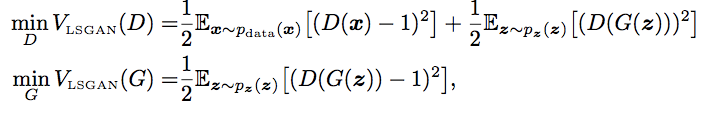
\includegraphics{pictures/lsgan.png}
\#\#\#\# \textbf{作业}:
在这里,请在下方补充L2Loss的代码来实现L2损失来优化上面的目标.并使用这个loss函数在mnist数据集上训练LSGAN,并显示训练的效果图片及loss变化曲线.

提示:忽略上图的1/2.L2损失即MSEloss(均方误差),传入两个参数input\_是指判别器D预测为``真实''的概率值(size为batch\_size*1),target为标签1或0(size为batch\_size*1).只允许使用pytorch和python的运算实现(不能直接调用MSEloss)

    \begin{Verbatim}[commandchars=\\\{\}]
{\color{incolor}In [{\color{incolor}13}]:} \PY{k}{class} \PY{n+nc}{L2Loss}\PY{p}{(}\PY{n}{nn}\PY{o}{.}\PY{n}{Module}\PY{p}{)}\PY{p}{:}
             \PY{k}{def} \PY{n+nf}{\PYZus{}\PYZus{}init\PYZus{}\PYZus{}}\PY{p}{(}\PY{n+nb+bp}{self}\PY{p}{)}\PY{p}{:}
                 \PY{n+nb}{super}\PY{p}{(}\PY{n}{L2Loss}\PY{p}{,} \PY{n+nb+bp}{self}\PY{p}{)}\PY{o}{.}\PY{n+nf+fm}{\PYZus{}\PYZus{}init\PYZus{}\PYZus{}}\PY{p}{(}\PY{p}{)}
             
             \PY{k}{def} \PY{n+nf}{forward}\PY{p}{(}\PY{n+nb+bp}{self}\PY{p}{,} \PY{n}{input\PYZus{}}\PY{p}{,} \PY{n}{target}\PY{p}{)}\PY{p}{:}
                 \PY{l+s+sd}{\PYZdq{}\PYZdq{}\PYZdq{}}
         \PY{l+s+sd}{        input\PYZus{}: (batch\PYZus{}size*1) }
         \PY{l+s+sd}{        target: (batch\PYZus{}size*1) labels, 1 or 0}
         \PY{l+s+sd}{        \PYZdq{}\PYZdq{}\PYZdq{}}
                 \PY{k}{return} \PY{p}{(}\PY{p}{(}\PY{n}{input\PYZus{}} \PY{o}{\PYZhy{}} \PY{n}{target}\PY{p}{)} \PY{o}{*}\PY{o}{*} \PY{l+m+mi}{2}\PY{p}{)}\PY{o}{.}\PY{n}{mean}\PY{p}{(}\PY{p}{)}
\end{Verbatim}


    完成上方代码后,使用所写的L2Loss在mnist数据集上训练DCGAN.

    \begin{Verbatim}[commandchars=\\\{\}]
{\color{incolor}In [{\color{incolor}14}]:} \PY{c+c1}{\PYZsh{} hyper params}
         
         \PY{c+c1}{\PYZsh{} z dim}
         \PY{n}{latent\PYZus{}dim} \PY{o}{=} \PY{l+m+mi}{100}
         
         \PY{c+c1}{\PYZsh{} image size and channel}
         \PY{n}{image\PYZus{}size}\PY{o}{=}\PY{l+m+mi}{32}
         \PY{n}{image\PYZus{}channel}\PY{o}{=}\PY{l+m+mi}{1}
         
         \PY{c+c1}{\PYZsh{} Adam lr and betas}
         \PY{n}{learning\PYZus{}rate} \PY{o}{=} \PY{l+m+mf}{0.0002}
         \PY{n}{betas} \PY{o}{=} \PY{p}{(}\PY{l+m+mf}{0.5}\PY{p}{,} \PY{l+m+mf}{0.999}\PY{p}{)}
         
         \PY{c+c1}{\PYZsh{} epochs and batch size}
         \PY{n}{n\PYZus{}epochs} \PY{o}{=} \PY{l+m+mi}{100}
         \PY{n}{batch\PYZus{}size} \PY{o}{=} \PY{l+m+mi}{32}
         
         \PY{c+c1}{\PYZsh{} device : cpu or cuda:0/1/2/3}
         \PY{n}{device} \PY{o}{=} \PY{n}{torch}\PY{o}{.}\PY{n}{device}\PY{p}{(}\PY{l+s+s1}{\PYZsq{}}\PY{l+s+s1}{cuda:0}\PY{l+s+s1}{\PYZsq{}}\PY{p}{)}
         
         \PY{c+c1}{\PYZsh{} mnist dataset and dataloader}
         \PY{n}{train\PYZus{}dataset} \PY{o}{=} \PY{n}{load\PYZus{}mnist\PYZus{}data}\PY{p}{(}\PY{p}{)}
         \PY{n}{trainloader} \PY{o}{=} \PY{n}{torch}\PY{o}{.}\PY{n}{utils}\PY{o}{.}\PY{n}{data}\PY{o}{.}\PY{n}{DataLoader}\PY{p}{(}\PY{n}{train\PYZus{}dataset}\PY{p}{,} \PY{n}{batch\PYZus{}size}\PY{o}{=}\PY{n}{batch\PYZus{}size}\PY{p}{,} \PY{n}{shuffle}\PY{o}{=}\PY{k+kc}{True}\PY{p}{)}
         
         \PY{c+c1}{\PYZsh{} use L2Loss as loss function}
         \PY{n}{l2loss} \PY{o}{=} \PY{n}{L2Loss}\PY{p}{(}\PY{p}{)}\PY{o}{.}\PY{n}{to}\PY{p}{(}\PY{n}{device}\PY{p}{)}
         
         \PY{c+c1}{\PYZsh{} G and D model, use DCGAN}
         \PY{n}{G} \PY{o}{=} \PY{n}{DCGenerator}\PY{p}{(}\PY{n}{image\PYZus{}size}\PY{o}{=}\PY{n}{image\PYZus{}size}\PY{p}{,} \PY{n}{latent\PYZus{}dim}\PY{o}{=}\PY{n}{latent\PYZus{}dim}\PY{p}{,} \PY{n}{output\PYZus{}channel}\PY{o}{=}\PY{n}{image\PYZus{}channel}\PY{p}{)}\PY{o}{.}\PY{n}{to}\PY{p}{(}\PY{n}{device}\PY{p}{)}
         \PY{n}{D} \PY{o}{=} \PY{n}{DCDiscriminator}\PY{p}{(}\PY{n}{image\PYZus{}size}\PY{o}{=}\PY{n}{image\PYZus{}size}\PY{p}{,} \PY{n}{input\PYZus{}channel}\PY{o}{=}\PY{n}{image\PYZus{}channel}\PY{p}{)}\PY{o}{.}\PY{n}{to}\PY{p}{(}\PY{n}{device}\PY{p}{)}
         
         \PY{c+c1}{\PYZsh{} G and D optimizer, use Adam or SGD}
         \PY{n}{G\PYZus{}optimizer} \PY{o}{=} \PY{n}{optim}\PY{o}{.}\PY{n}{Adam}\PY{p}{(}\PY{n}{G}\PY{o}{.}\PY{n}{parameters}\PY{p}{(}\PY{p}{)}\PY{p}{,} \PY{n}{lr}\PY{o}{=}\PY{n}{learning\PYZus{}rate}\PY{p}{,} \PY{n}{betas}\PY{o}{=}\PY{n}{betas}\PY{p}{)}
         \PY{n}{D\PYZus{}optimizer} \PY{o}{=} \PY{n}{optim}\PY{o}{.}\PY{n}{Adam}\PY{p}{(}\PY{n}{D}\PY{o}{.}\PY{n}{parameters}\PY{p}{(}\PY{p}{)}\PY{p}{,} \PY{n}{lr}\PY{o}{=}\PY{n}{learning\PYZus{}rate}\PY{p}{,} \PY{n}{betas}\PY{o}{=}\PY{n}{betas}\PY{p}{)}
\end{Verbatim}


    \begin{Verbatim}[commandchars=\\\{\}]
{\color{incolor}In [{\color{incolor}15}]:} \PY{n}{d\PYZus{}loss\PYZus{}hist}\PY{p}{,} \PY{n}{g\PYZus{}loss\PYZus{}hist} \PY{o}{=} \PY{n}{run\PYZus{}gan}\PY{p}{(}\PY{n}{trainloader}\PY{p}{,} \PY{n}{G}\PY{p}{,} \PY{n}{D}\PY{p}{,} \PY{n}{G\PYZus{}optimizer}\PY{p}{,} \PY{n}{D\PYZus{}optimizer}\PY{p}{,} \PY{n}{l2loss}\PY{p}{,} \PY{n}{n\PYZus{}epochs}\PY{p}{,} \PY{n}{device}\PY{p}{,} 
                                            \PY{n}{latent\PYZus{}dim}\PY{p}{)}
         \PY{n}{loss\PYZus{}plot}\PY{p}{(}\PY{n}{d\PYZus{}loss\PYZus{}hist}\PY{p}{,} \PY{n}{g\PYZus{}loss\PYZus{}hist}\PY{p}{)}
\end{Verbatim}


    \begin{Verbatim}[commandchars=\\\{\}]
Epoch 0: Train D loss: 0.0850, G loss: 0.9358

    \end{Verbatim}

    \begin{center}
    \adjustimage{max size={0.9\linewidth}{0.9\paperheight}}{output_39_1.png}
    \end{center}
    { \hspace*{\fill} \\}
    
    \begin{Verbatim}[commandchars=\\\{\}]
Epoch 1: Train D loss: 0.0339, G loss: 0.9883
Epoch 2: Train D loss: 0.0089, G loss: 0.9966
Epoch 3: Train D loss: 0.0001, G loss: 1.0000
Epoch 4: Train D loss: 0.0000, G loss: 1.0000
Epoch 5: Train D loss: 0.0000, G loss: 0.9999
Epoch 6: Train D loss: 0.1980, G loss: 0.9983
Epoch 7: Train D loss: 1.0000, G loss: 1.0000
Epoch 8: Train D loss: 0.9999, G loss: 1.0000
Epoch 9: Train D loss: 0.9998, G loss: 1.0000

    \end{Verbatim}

    \begin{center}
    \adjustimage{max size={0.9\linewidth}{0.9\paperheight}}{output_39_3.png}
    \end{center}
    { \hspace*{\fill} \\}
    
    \begin{Verbatim}[commandchars=\\\{\}]
Epoch 10: Train D loss: 0.4128, G loss: 0.9972
Epoch 11: Train D loss: 0.0458, G loss: 0.9910
Epoch 12: Train D loss: 0.0854, G loss: 0.9669
Epoch 13: Train D loss: 0.2655, G loss: 0.8347
Epoch 14: Train D loss: 0.3056, G loss: 0.6851
Epoch 15: Train D loss: 0.3189, G loss: 0.7072
Epoch 16: Train D loss: 0.2210, G loss: 0.6810
Epoch 17: Train D loss: 0.2715, G loss: 0.6473
Epoch 18: Train D loss: 0.2267, G loss: 0.6472
Epoch 19: Train D loss: 0.2314, G loss: 0.6481

    \end{Verbatim}

    \begin{center}
    \adjustimage{max size={0.9\linewidth}{0.9\paperheight}}{output_39_5.png}
    \end{center}
    { \hspace*{\fill} \\}
    
    \begin{Verbatim}[commandchars=\\\{\}]
Epoch 20: Train D loss: 0.2162, G loss: 0.6572
Epoch 21: Train D loss: 0.2415, G loss: 0.6667
Epoch 22: Train D loss: 0.2197, G loss: 0.6622
Epoch 23: Train D loss: 0.2128, G loss: 0.6723
Epoch 24: Train D loss: 0.1959, G loss: 0.6868
Epoch 25: Train D loss: 0.1813, G loss: 0.6975
Epoch 26: Train D loss: 0.1652, G loss: 0.7022
Epoch 27: Train D loss: 0.1281, G loss: 0.7549
Epoch 28: Train D loss: 0.1265, G loss: 0.7610
Epoch 29: Train D loss: 0.1125, G loss: 0.7719

    \end{Verbatim}

    \begin{center}
    \adjustimage{max size={0.9\linewidth}{0.9\paperheight}}{output_39_7.png}
    \end{center}
    { \hspace*{\fill} \\}
    
    \begin{Verbatim}[commandchars=\\\{\}]
Epoch 30: Train D loss: 0.0799, G loss: 0.8024
Epoch 31: Train D loss: 0.0694, G loss: 0.8223
Epoch 32: Train D loss: 0.0946, G loss: 0.8116
Epoch 33: Train D loss: 0.0517, G loss: 0.8531
Epoch 34: Train D loss: 0.0633, G loss: 0.8562
Epoch 35: Train D loss: 0.0824, G loss: 0.8502
Epoch 36: Train D loss: 0.0369, G loss: 0.8721
Epoch 37: Train D loss: 0.0184, G loss: 0.8933
Epoch 38: Train D loss: 0.0966, G loss: 0.8547
Epoch 39: Train D loss: 0.0277, G loss: 0.8822

    \end{Verbatim}

    \begin{center}
    \adjustimage{max size={0.9\linewidth}{0.9\paperheight}}{output_39_9.png}
    \end{center}
    { \hspace*{\fill} \\}
    
    \begin{Verbatim}[commandchars=\\\{\}]
Epoch 40: Train D loss: 0.0110, G loss: 0.9106
Epoch 41: Train D loss: 0.0113, G loss: 0.9162
Epoch 42: Train D loss: 0.1998, G loss: 0.8257
Epoch 43: Train D loss: 0.0212, G loss: 0.8944
Epoch 44: Train D loss: 0.0118, G loss: 0.9129
Epoch 45: Train D loss: 0.0084, G loss: 0.9272
Epoch 46: Train D loss: 0.0072, G loss: 0.9320
Epoch 47: Train D loss: 0.2002, G loss: 0.9342
Epoch 48: Train D loss: 0.6590, G loss: 0.9179
Epoch 49: Train D loss: 0.0679, G loss: 0.8830

    \end{Verbatim}

    \begin{center}
    \adjustimage{max size={0.9\linewidth}{0.9\paperheight}}{output_39_11.png}
    \end{center}
    { \hspace*{\fill} \\}
    
    \begin{Verbatim}[commandchars=\\\{\}]
Epoch 50: Train D loss: 0.0122, G loss: 0.9184
Epoch 51: Train D loss: 0.1843, G loss: 0.8181
Epoch 52: Train D loss: 0.1346, G loss: 0.8098
Epoch 53: Train D loss: 0.0217, G loss: 0.9110
Epoch 54: Train D loss: 0.0082, G loss: 0.9325
Epoch 55: Train D loss: 0.0085, G loss: 0.9302
Epoch 56: Train D loss: 0.0059, G loss: 0.9357
Epoch 57: Train D loss: 0.0046, G loss: 0.9492
Epoch 58: Train D loss: 0.0049, G loss: 0.9488
Epoch 59: Train D loss: 0.0035, G loss: 0.9508

    \end{Verbatim}

    \begin{center}
    \adjustimage{max size={0.9\linewidth}{0.9\paperheight}}{output_39_13.png}
    \end{center}
    { \hspace*{\fill} \\}
    
    \begin{Verbatim}[commandchars=\\\{\}]
Epoch 60: Train D loss: 0.0029, G loss: 0.9561
Epoch 61: Train D loss: 0.0029, G loss: 0.9566
Epoch 62: Train D loss: 0.8149, G loss: 0.9807
Epoch 63: Train D loss: 1.0000, G loss: 1.0000
Epoch 64: Train D loss: 1.0000, G loss: 1.0000
Epoch 65: Train D loss: 1.0000, G loss: 1.0000
Epoch 66: Train D loss: 1.0000, G loss: 1.0000
Epoch 67: Train D loss: 1.0000, G loss: 1.0000
Epoch 68: Train D loss: 1.0000, G loss: 1.0000
Epoch 69: Train D loss: 1.0000, G loss: 1.0000

    \end{Verbatim}

    \begin{center}
    \adjustimage{max size={0.9\linewidth}{0.9\paperheight}}{output_39_15.png}
    \end{center}
    { \hspace*{\fill} \\}
    
    \begin{Verbatim}[commandchars=\\\{\}]
Epoch 70: Train D loss: 1.0000, G loss: 1.0000
Epoch 71: Train D loss: 1.0000, G loss: 1.0000
Epoch 72: Train D loss: 1.0000, G loss: 1.0000
Epoch 73: Train D loss: 1.0000, G loss: 1.0000
Epoch 74: Train D loss: 1.0000, G loss: 1.0000
Epoch 75: Train D loss: 1.0000, G loss: 1.0000
Epoch 76: Train D loss: 1.0000, G loss: 1.0000
Epoch 77: Train D loss: 1.0000, G loss: 1.0000
Epoch 78: Train D loss: 1.0000, G loss: 1.0000
Epoch 79: Train D loss: 1.0000, G loss: 1.0000

    \end{Verbatim}

    \begin{center}
    \adjustimage{max size={0.9\linewidth}{0.9\paperheight}}{output_39_17.png}
    \end{center}
    { \hspace*{\fill} \\}
    
    \begin{Verbatim}[commandchars=\\\{\}]
Epoch 80: Train D loss: 1.0000, G loss: 1.0000
Epoch 81: Train D loss: 1.0000, G loss: 1.0000
Epoch 82: Train D loss: 1.0000, G loss: 1.0000
Epoch 83: Train D loss: 1.0000, G loss: 1.0000
Epoch 84: Train D loss: 1.0000, G loss: 1.0000
Epoch 85: Train D loss: 1.0000, G loss: 1.0000
Epoch 86: Train D loss: 1.0000, G loss: 1.0000
Epoch 87: Train D loss: 1.0000, G loss: 1.0000
Epoch 88: Train D loss: 1.0000, G loss: 1.0000
Epoch 89: Train D loss: 1.0000, G loss: 1.0000

    \end{Verbatim}

    \begin{center}
    \adjustimage{max size={0.9\linewidth}{0.9\paperheight}}{output_39_19.png}
    \end{center}
    { \hspace*{\fill} \\}
    
    \begin{Verbatim}[commandchars=\\\{\}]
Epoch 90: Train D loss: 1.0000, G loss: 1.0000
Epoch 91: Train D loss: 1.0000, G loss: 1.0000
Epoch 92: Train D loss: 1.0000, G loss: 1.0000
Epoch 93: Train D loss: 1.0000, G loss: 1.0000
Epoch 94: Train D loss: 1.0000, G loss: 1.0000
Epoch 95: Train D loss: 1.0000, G loss: 1.0000
Epoch 96: Train D loss: 1.0000, G loss: 1.0000
Epoch 97: Train D loss: 1.0000, G loss: 1.0000
Epoch 98: Train D loss: 1.0000, G loss: 1.0000
Epoch 99: Train D loss: 1.0000, G loss: 1.0000

    \end{Verbatim}

    \begin{center}
    \adjustimage{max size={0.9\linewidth}{0.9\paperheight}}{output_39_21.png}
    \end{center}
    { \hspace*{\fill} \\}
    
    \begin{center}
    \adjustimage{max size={0.9\linewidth}{0.9\paperheight}}{output_39_22.png}
    \end{center}
    { \hspace*{\fill} \\}
    
    \hypertarget{wgan}{%
\subsection{WGAN}\label{wgan}}

    GAN依然存在着训练不稳定,模式崩溃(collapse
mode,可以理解为生成的图片多样性极低)的问题(我们的数据集不一定能体现出来).WGAN(Wasserstein
GAN)将传统GAN中拟合的JS散度改为Wasserstein距离.WGAN一定程度上解决了GAN训练不稳定以及模式奔溃的问题.

WGAN的判别器的优化目标变为,在满足Lipschitz连续的条件(我们可以限制w不超过某个范围来满足)下,最大化
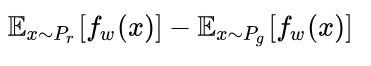
\includegraphics{pictures/wgan1.png}
而它会近似于真实分布与生成分布之间的Wasserstein距离.所以我们D和G的loss函数变为:
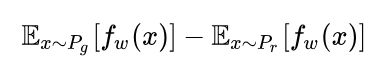
\includegraphics{pictures/wgan3.png}
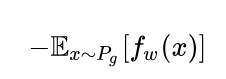
\includegraphics{pictures/wgan2.png}

具体到在实现上,WGAN主要有3点改变: - 判别器D最后一层去掉sigmoid -
生成器G和判别器的loss不使用log -
每次更新判别器D后,将参数的绝对值截断到某一个固定常数c

所以我们主要重写了WGAN的训练函数,在这里,网络结构使用\emph{去除Sigmoid的DCGAN}(注意初始化D时将sigmoid设置为False来去掉最后一层sigmoid).

下面是WGAN的代码实现.加入了两个参数,n\_d表示每训练一次G训练D的次数,weight\_clip表示截断的常数.

    \begin{Verbatim}[commandchars=\\\{\}]
{\color{incolor}In [{\color{incolor}16}]:} \PY{k}{def} \PY{n+nf}{wgan\PYZus{}train}\PY{p}{(}\PY{n}{trainloader}\PY{p}{,} \PY{n}{G}\PY{p}{,} \PY{n}{D}\PY{p}{,} \PY{n}{G\PYZus{}optimizer}\PY{p}{,} \PY{n}{D\PYZus{}optimizer}\PY{p}{,} \PY{n}{device}\PY{p}{,} \PY{n}{z\PYZus{}dim}\PY{p}{,} \PY{n}{n\PYZus{}d}\PY{o}{=}\PY{l+m+mi}{2}\PY{p}{,} \PY{n}{weight\PYZus{}clip}\PY{o}{=}\PY{l+m+mf}{0.01}\PY{p}{)}\PY{p}{:}
             
             \PY{l+s+sd}{\PYZdq{}\PYZdq{}\PYZdq{}}
         \PY{l+s+sd}{    n\PYZus{}d: the number of iterations of D update per G update iteration}
         \PY{l+s+sd}{    weight\PYZus{}clip: the clipping parameters}
         \PY{l+s+sd}{    \PYZdq{}\PYZdq{}\PYZdq{}}
             
             \PY{n}{D}\PY{o}{.}\PY{n}{train}\PY{p}{(}\PY{p}{)}
             \PY{n}{G}\PY{o}{.}\PY{n}{train}\PY{p}{(}\PY{p}{)}
             
             \PY{n}{D\PYZus{}total\PYZus{}loss} \PY{o}{=} \PY{l+m+mi}{0}
             \PY{n}{G\PYZus{}total\PYZus{}loss} \PY{o}{=} \PY{l+m+mi}{0}
             
             \PY{k}{for} \PY{n}{i}\PY{p}{,} \PY{p}{(}\PY{n}{x}\PY{p}{,} \PY{n}{\PYZus{}}\PY{p}{)} \PY{o+ow}{in} \PY{n+nb}{enumerate}\PY{p}{(}\PY{n}{trainloader}\PY{p}{)}\PY{p}{:}
                 
                 \PY{n}{x} \PY{o}{=} \PY{n}{x}\PY{o}{.}\PY{n}{to}\PY{p}{(}\PY{n}{device}\PY{p}{)}
                 
                 \PY{c+c1}{\PYZsh{} update D network}
                 \PY{c+c1}{\PYZsh{} D optimizer zero grads}
                 \PY{n}{D\PYZus{}optimizer}\PY{o}{.}\PY{n}{zero\PYZus{}grad}\PY{p}{(}\PY{p}{)}
                 
                 \PY{c+c1}{\PYZsh{} D real loss from real images}
                 \PY{n}{d\PYZus{}real} \PY{o}{=} \PY{n}{D}\PY{p}{(}\PY{n}{x}\PY{p}{)}
                 \PY{n}{d\PYZus{}real\PYZus{}loss} \PY{o}{=} \PY{o}{\PYZhy{}} \PY{n}{d\PYZus{}real}\PY{o}{.}\PY{n}{mean}\PY{p}{(}\PY{p}{)}
                 
                 \PY{c+c1}{\PYZsh{} D fake loss from fake images generated by G}
                 \PY{n}{z} \PY{o}{=} \PY{n}{torch}\PY{o}{.}\PY{n}{rand}\PY{p}{(}\PY{n}{x}\PY{o}{.}\PY{n}{size}\PY{p}{(}\PY{l+m+mi}{0}\PY{p}{)}\PY{p}{,} \PY{n}{z\PYZus{}dim}\PY{p}{)}\PY{o}{.}\PY{n}{to}\PY{p}{(}\PY{n}{device}\PY{p}{)}
                 \PY{n}{g\PYZus{}z} \PY{o}{=} \PY{n}{G}\PY{p}{(}\PY{n}{z}\PY{p}{)}
                 \PY{n}{d\PYZus{}fake} \PY{o}{=} \PY{n}{D}\PY{p}{(}\PY{n}{g\PYZus{}z}\PY{p}{)}
                 \PY{n}{d\PYZus{}fake\PYZus{}loss} \PY{o}{=} \PY{n}{d\PYZus{}fake}\PY{o}{.}\PY{n}{mean}\PY{p}{(}\PY{p}{)}
                 
                 \PY{c+c1}{\PYZsh{} D backward and step}
                 \PY{n}{d\PYZus{}loss} \PY{o}{=} \PY{n}{d\PYZus{}real\PYZus{}loss} \PY{o}{+} \PY{n}{d\PYZus{}fake\PYZus{}loss}
                 \PY{n}{d\PYZus{}loss}\PY{o}{.}\PY{n}{backward}\PY{p}{(}\PY{p}{)}
                 \PY{n}{D\PYZus{}optimizer}\PY{o}{.}\PY{n}{step}\PY{p}{(}\PY{p}{)}
                 
                 \PY{c+c1}{\PYZsh{} D weight clip}
                 \PY{k}{for} \PY{n}{params} \PY{o+ow}{in} \PY{n}{D}\PY{o}{.}\PY{n}{parameters}\PY{p}{(}\PY{p}{)}\PY{p}{:}
                     \PY{n}{params}\PY{o}{.}\PY{n}{data}\PY{o}{.}\PY{n}{clamp\PYZus{}}\PY{p}{(}\PY{o}{\PYZhy{}}\PY{n}{weight\PYZus{}clip}\PY{p}{,} \PY{n}{weight\PYZus{}clip}\PY{p}{)}
                     
                 \PY{n}{D\PYZus{}total\PYZus{}loss} \PY{o}{+}\PY{o}{=} \PY{n}{d\PYZus{}loss}\PY{o}{.}\PY{n}{item}\PY{p}{(}\PY{p}{)}
         
                 \PY{c+c1}{\PYZsh{} update G network}
                 \PY{k}{if} \PY{p}{(}\PY{n}{i} \PY{o}{+} \PY{l+m+mi}{1}\PY{p}{)} \PY{o}{\PYZpc{}} \PY{n}{n\PYZus{}d} \PY{o}{==} \PY{l+m+mi}{0}\PY{p}{:}
                     \PY{c+c1}{\PYZsh{} G optimizer zero grads}
                     \PY{n}{G\PYZus{}optimizer}\PY{o}{.}\PY{n}{zero\PYZus{}grad}\PY{p}{(}\PY{p}{)}
         
                     \PY{c+c1}{\PYZsh{} G loss}
                     \PY{n}{g\PYZus{}z} \PY{o}{=} \PY{n}{G}\PY{p}{(}\PY{n}{z}\PY{p}{)}
                     \PY{n}{d\PYZus{}fake} \PY{o}{=} \PY{n}{D}\PY{p}{(}\PY{n}{g\PYZus{}z}\PY{p}{)}
                     \PY{n}{g\PYZus{}loss} \PY{o}{=} \PY{o}{\PYZhy{}} \PY{n}{d\PYZus{}fake}\PY{o}{.}\PY{n}{mean}\PY{p}{(}\PY{p}{)}
         
                     \PY{c+c1}{\PYZsh{} G backward and step}
                     \PY{n}{g\PYZus{}loss}\PY{o}{.}\PY{n}{backward}\PY{p}{(}\PY{p}{)}
                     \PY{n}{G\PYZus{}optimizer}\PY{o}{.}\PY{n}{step}\PY{p}{(}\PY{p}{)}
                     
                     \PY{n}{G\PYZus{}total\PYZus{}loss} \PY{o}{+}\PY{o}{=} \PY{n}{g\PYZus{}loss}\PY{o}{.}\PY{n}{item}\PY{p}{(}\PY{p}{)}
             
             \PY{k}{return} \PY{n}{D\PYZus{}total\PYZus{}loss} \PY{o}{/} \PY{n+nb}{len}\PY{p}{(}\PY{n}{trainloader}\PY{p}{)}\PY{p}{,} \PY{n}{G\PYZus{}total\PYZus{}loss} \PY{o}{*} \PY{n}{n\PYZus{}d} \PY{o}{/} \PY{n+nb}{len}\PY{p}{(}\PY{n}{trainloader}\PY{p}{)}
\end{Verbatim}


    \begin{Verbatim}[commandchars=\\\{\}]
{\color{incolor}In [{\color{incolor}17}]:} \PY{k}{def} \PY{n+nf}{run\PYZus{}wgan}\PY{p}{(}\PY{n}{trainloader}\PY{p}{,} \PY{n}{G}\PY{p}{,} \PY{n}{D}\PY{p}{,} \PY{n}{G\PYZus{}optimizer}\PY{p}{,} \PY{n}{D\PYZus{}optimizer}\PY{p}{,} \PY{n}{n\PYZus{}epochs}\PY{p}{,} \PY{n}{device}\PY{p}{,} \PY{n}{latent\PYZus{}dim}\PY{p}{,} \PY{n}{n\PYZus{}d}\PY{p}{,} \PY{n}{weight\PYZus{}clip}\PY{p}{)}\PY{p}{:}
             \PY{n}{d\PYZus{}loss\PYZus{}hist} \PY{o}{=} \PY{p}{[}\PY{p}{]}
             \PY{n}{g\PYZus{}loss\PYZus{}hist} \PY{o}{=} \PY{p}{[}\PY{p}{]}
         
             \PY{k}{for} \PY{n}{epoch} \PY{o+ow}{in} \PY{n+nb}{range}\PY{p}{(}\PY{n}{n\PYZus{}epochs}\PY{p}{)}\PY{p}{:}
                 \PY{n}{d\PYZus{}loss}\PY{p}{,} \PY{n}{g\PYZus{}loss} \PY{o}{=} \PY{n}{wgan\PYZus{}train}\PY{p}{(}\PY{n}{trainloader}\PY{p}{,} \PY{n}{G}\PY{p}{,} \PY{n}{D}\PY{p}{,} \PY{n}{G\PYZus{}optimizer}\PY{p}{,} \PY{n}{D\PYZus{}optimizer}\PY{p}{,} \PY{n}{device}\PY{p}{,} 
                                        \PY{n}{z\PYZus{}dim}\PY{o}{=}\PY{n}{latent\PYZus{}dim}\PY{p}{,} \PY{n}{n\PYZus{}d}\PY{o}{=}\PY{n}{n\PYZus{}d}\PY{p}{,} \PY{n}{weight\PYZus{}clip}\PY{o}{=}\PY{n}{weight\PYZus{}clip}\PY{p}{)}
                 \PY{n+nb}{print}\PY{p}{(}\PY{l+s+s1}{\PYZsq{}}\PY{l+s+s1}{Epoch }\PY{l+s+si}{\PYZob{}\PYZcb{}}\PY{l+s+s1}{: Train D loss: }\PY{l+s+si}{\PYZob{}:.4f\PYZcb{}}\PY{l+s+s1}{, G loss: }\PY{l+s+si}{\PYZob{}:.4f\PYZcb{}}\PY{l+s+s1}{\PYZsq{}}\PY{o}{.}\PY{n}{format}\PY{p}{(}\PY{n}{epoch}\PY{p}{,} \PY{n}{d\PYZus{}loss}\PY{p}{,} \PY{n}{g\PYZus{}loss}\PY{p}{)}\PY{p}{)}
         
                 \PY{n}{d\PYZus{}loss\PYZus{}hist}\PY{o}{.}\PY{n}{append}\PY{p}{(}\PY{n}{d\PYZus{}loss}\PY{p}{)}
                 \PY{n}{g\PYZus{}loss\PYZus{}hist}\PY{o}{.}\PY{n}{append}\PY{p}{(}\PY{n}{g\PYZus{}loss}\PY{p}{)}
         
                 \PY{k}{if} \PY{n}{epoch} \PY{o}{==} \PY{l+m+mi}{0} \PY{o+ow}{or} \PY{p}{(}\PY{n}{epoch} \PY{o}{+} \PY{l+m+mi}{1}\PY{p}{)} \PY{o}{\PYZpc{}} \PY{l+m+mi}{10} \PY{o}{==} \PY{l+m+mi}{0}\PY{p}{:}
                     \PY{n}{visualize\PYZus{}results}\PY{p}{(}\PY{n}{G}\PY{p}{,} \PY{n}{device}\PY{p}{,} \PY{n}{latent\PYZus{}dim}\PY{p}{)} 
             
             \PY{k}{return} \PY{n}{d\PYZus{}loss\PYZus{}hist}\PY{p}{,} \PY{n}{g\PYZus{}loss\PYZus{}hist}
\end{Verbatim}


    接下来让我们使用写好的run\_wgan来跑我们的家具(椅子)数据集,看看效果如何.

    \begin{Verbatim}[commandchars=\\\{\}]
{\color{incolor}In [{\color{incolor}18}]:} \PY{c+c1}{\PYZsh{} hyper params}
         
         \PY{c+c1}{\PYZsh{} z dim}
         \PY{n}{latent\PYZus{}dim} \PY{o}{=} \PY{l+m+mi}{100}
         
         \PY{c+c1}{\PYZsh{} image size and channel}
         \PY{n}{image\PYZus{}size}\PY{o}{=}\PY{l+m+mi}{32}
         \PY{n}{image\PYZus{}channel}\PY{o}{=}\PY{l+m+mi}{3}
         
         \PY{c+c1}{\PYZsh{} Adam lr and betas}
         \PY{n}{learning\PYZus{}rate} \PY{o}{=} \PY{l+m+mf}{0.0002}
         \PY{n}{betas} \PY{o}{=} \PY{p}{(}\PY{l+m+mf}{0.5}\PY{p}{,} \PY{l+m+mf}{0.999}\PY{p}{)}
         
         \PY{c+c1}{\PYZsh{} epochs and batch size}
         \PY{n}{n\PYZus{}epochs} \PY{o}{=} \PY{l+m+mi}{300}
         \PY{n}{batch\PYZus{}size} \PY{o}{=} \PY{l+m+mi}{32}
         
         \PY{c+c1}{\PYZsh{} n\PYZus{}d: the number of iterations of D update per G update iteration}
         \PY{n}{n\PYZus{}d} \PY{o}{=} \PY{l+m+mi}{2}
         \PY{n}{weight\PYZus{}clip}\PY{o}{=}\PY{l+m+mf}{0.01}
         
         \PY{c+c1}{\PYZsh{} device : cpu or cuda:0/1/2/3}
         \PY{n}{device} \PY{o}{=} \PY{n}{torch}\PY{o}{.}\PY{n}{device}\PY{p}{(}\PY{l+s+s1}{\PYZsq{}}\PY{l+s+s1}{cuda:0}\PY{l+s+s1}{\PYZsq{}}\PY{p}{)}
         
         \PY{c+c1}{\PYZsh{} mnist dataset and dataloader}
         \PY{n}{train\PYZus{}dataset} \PY{o}{=} \PY{n}{load\PYZus{}furniture\PYZus{}data}\PY{p}{(}\PY{p}{)}
         \PY{n}{trainloader} \PY{o}{=} \PY{n}{torch}\PY{o}{.}\PY{n}{utils}\PY{o}{.}\PY{n}{data}\PY{o}{.}\PY{n}{DataLoader}\PY{p}{(}\PY{n}{train\PYZus{}dataset}\PY{p}{,} \PY{n}{batch\PYZus{}size}\PY{o}{=}\PY{n}{batch\PYZus{}size}\PY{p}{,} \PY{n}{shuffle}\PY{o}{=}\PY{k+kc}{True}\PY{p}{)}
         
         \PY{c+c1}{\PYZsh{} G and D model, use DCGAN, note that sigmoid is removed in D}
         \PY{n}{G} \PY{o}{=} \PY{n}{DCGenerator}\PY{p}{(}\PY{n}{image\PYZus{}size}\PY{o}{=}\PY{n}{image\PYZus{}size}\PY{p}{,} \PY{n}{latent\PYZus{}dim}\PY{o}{=}\PY{n}{latent\PYZus{}dim}\PY{p}{,} \PY{n}{output\PYZus{}channel}\PY{o}{=}\PY{n}{image\PYZus{}channel}\PY{p}{)}\PY{o}{.}\PY{n}{to}\PY{p}{(}\PY{n}{device}\PY{p}{)}
         \PY{n}{D} \PY{o}{=} \PY{n}{DCDiscriminator}\PY{p}{(}\PY{n}{image\PYZus{}size}\PY{o}{=}\PY{n}{image\PYZus{}size}\PY{p}{,} \PY{n}{input\PYZus{}channel}\PY{o}{=}\PY{n}{image\PYZus{}channel}\PY{p}{,} \PY{n}{sigmoid}\PY{o}{=}\PY{k+kc}{False}\PY{p}{)}\PY{o}{.}\PY{n}{to}\PY{p}{(}\PY{n}{device}\PY{p}{)}
         
         \PY{c+c1}{\PYZsh{} G and D optimizer, use Adam or SGD}
         \PY{n}{G\PYZus{}optimizer} \PY{o}{=} \PY{n}{optim}\PY{o}{.}\PY{n}{Adam}\PY{p}{(}\PY{n}{G}\PY{o}{.}\PY{n}{parameters}\PY{p}{(}\PY{p}{)}\PY{p}{,} \PY{n}{lr}\PY{o}{=}\PY{n}{learning\PYZus{}rate}\PY{p}{,} \PY{n}{betas}\PY{o}{=}\PY{n}{betas}\PY{p}{)}
         \PY{n}{D\PYZus{}optimizer} \PY{o}{=} \PY{n}{optim}\PY{o}{.}\PY{n}{Adam}\PY{p}{(}\PY{n}{D}\PY{o}{.}\PY{n}{parameters}\PY{p}{(}\PY{p}{)}\PY{p}{,} \PY{n}{lr}\PY{o}{=}\PY{n}{learning\PYZus{}rate}\PY{p}{,} \PY{n}{betas}\PY{o}{=}\PY{n}{betas}\PY{p}{)}
         
         \PY{n}{d\PYZus{}loss\PYZus{}hist}\PY{p}{,} \PY{n}{g\PYZus{}loss\PYZus{}hist} \PY{o}{=} \PY{n}{run\PYZus{}wgan}\PY{p}{(}\PY{n}{trainloader}\PY{p}{,} \PY{n}{G}\PY{p}{,} \PY{n}{D}\PY{p}{,} \PY{n}{G\PYZus{}optimizer}\PY{p}{,} \PY{n}{D\PYZus{}optimizer}\PY{p}{,} \PY{n}{n\PYZus{}epochs}\PY{p}{,} \PY{n}{device}\PY{p}{,} 
                                             \PY{n}{latent\PYZus{}dim}\PY{p}{,} \PY{n}{n\PYZus{}d}\PY{p}{,} \PY{n}{weight\PYZus{}clip}\PY{p}{)}
\end{Verbatim}


    \begin{Verbatim}[commandchars=\\\{\}]
Epoch 0: Train D loss: 0.0210, G loss: -0.0007

    \end{Verbatim}

    \begin{center}
    \adjustimage{max size={0.9\linewidth}{0.9\paperheight}}{output_45_1.png}
    \end{center}
    { \hspace*{\fill} \\}
    
    \begin{Verbatim}[commandchars=\\\{\}]
Epoch 1: Train D loss: -0.0526, G loss: 0.0129
Epoch 2: Train D loss: -0.1158, G loss: 0.0771
Epoch 3: Train D loss: -0.2322, G loss: 0.1828
Epoch 4: Train D loss: -0.3840, G loss: 0.2651
Epoch 5: Train D loss: -0.5127, G loss: 0.3352
Epoch 6: Train D loss: -0.6154, G loss: 0.3958
Epoch 7: Train D loss: -0.5296, G loss: 0.3482
Epoch 8: Train D loss: -0.5814, G loss: 0.3981
Epoch 9: Train D loss: -0.6473, G loss: 0.3969

    \end{Verbatim}

    \begin{center}
    \adjustimage{max size={0.9\linewidth}{0.9\paperheight}}{output_45_3.png}
    \end{center}
    { \hspace*{\fill} \\}
    
    \begin{Verbatim}[commandchars=\\\{\}]
Epoch 10: Train D loss: -0.5214, G loss: 0.3830
Epoch 11: Train D loss: -0.5985, G loss: 0.4087
Epoch 12: Train D loss: -0.6966, G loss: 0.4560
Epoch 13: Train D loss: -0.5993, G loss: 0.4526
Epoch 14: Train D loss: -0.6478, G loss: 0.4761
Epoch 15: Train D loss: -0.7249, G loss: 0.4729
Epoch 16: Train D loss: -0.6600, G loss: 0.4592
Epoch 17: Train D loss: -0.6043, G loss: 0.4493
Epoch 18: Train D loss: -0.6826, G loss: 0.4750
Epoch 19: Train D loss: -0.6495, G loss: 0.4510

    \end{Verbatim}

    \begin{center}
    \adjustimage{max size={0.9\linewidth}{0.9\paperheight}}{output_45_5.png}
    \end{center}
    { \hspace*{\fill} \\}
    
    \begin{Verbatim}[commandchars=\\\{\}]
Epoch 20: Train D loss: -0.6669, G loss: 0.4692
Epoch 21: Train D loss: -0.5737, G loss: 0.4496
Epoch 22: Train D loss: -0.5842, G loss: 0.4300
Epoch 23: Train D loss: -0.6600, G loss: 0.4551
Epoch 24: Train D loss: -0.6336, G loss: 0.4372
Epoch 25: Train D loss: -0.5912, G loss: 0.4206
Epoch 26: Train D loss: -0.6134, G loss: 0.4436
Epoch 27: Train D loss: -0.6362, G loss: 0.4352
Epoch 28: Train D loss: -0.6273, G loss: 0.4218
Epoch 29: Train D loss: -0.6311, G loss: 0.4344

    \end{Verbatim}

    \begin{center}
    \adjustimage{max size={0.9\linewidth}{0.9\paperheight}}{output_45_7.png}
    \end{center}
    { \hspace*{\fill} \\}
    
    \begin{Verbatim}[commandchars=\\\{\}]
Epoch 30: Train D loss: -0.6558, G loss: 0.4361
Epoch 31: Train D loss: -0.5825, G loss: 0.4358
Epoch 32: Train D loss: -0.6214, G loss: 0.4444
Epoch 33: Train D loss: -0.6198, G loss: 0.4255
Epoch 34: Train D loss: -0.5761, G loss: 0.4267
Epoch 35: Train D loss: -0.6773, G loss: 0.4264
Epoch 36: Train D loss: -0.5675, G loss: 0.4091
Epoch 37: Train D loss: -0.6058, G loss: 0.3986
Epoch 38: Train D loss: -0.6099, G loss: 0.4057
Epoch 39: Train D loss: -0.5985, G loss: 0.3761

    \end{Verbatim}

    \begin{center}
    \adjustimage{max size={0.9\linewidth}{0.9\paperheight}}{output_45_9.png}
    \end{center}
    { \hspace*{\fill} \\}
    
    \begin{Verbatim}[commandchars=\\\{\}]
Epoch 40: Train D loss: -0.5728, G loss: 0.3691
Epoch 41: Train D loss: -0.6171, G loss: 0.3860
Epoch 42: Train D loss: -0.5872, G loss: 0.3847
Epoch 43: Train D loss: -0.5927, G loss: 0.3526
Epoch 44: Train D loss: -0.5930, G loss: 0.3700
Epoch 45: Train D loss: -0.5538, G loss: 0.3556
Epoch 46: Train D loss: -0.5687, G loss: 0.3681
Epoch 47: Train D loss: -0.5960, G loss: 0.3801
Epoch 48: Train D loss: -0.5643, G loss: 0.3496
Epoch 49: Train D loss: -0.5816, G loss: 0.3449

    \end{Verbatim}

    \begin{center}
    \adjustimage{max size={0.9\linewidth}{0.9\paperheight}}{output_45_11.png}
    \end{center}
    { \hspace*{\fill} \\}
    
    \begin{Verbatim}[commandchars=\\\{\}]
Epoch 50: Train D loss: -0.5871, G loss: 0.3503
Epoch 51: Train D loss: -0.5754, G loss: 0.3890
Epoch 52: Train D loss: -0.5961, G loss: 0.3546
Epoch 53: Train D loss: -0.4919, G loss: 0.3459
Epoch 54: Train D loss: -0.5785, G loss: 0.3664
Epoch 55: Train D loss: -0.5736, G loss: 0.3461
Epoch 56: Train D loss: -0.5143, G loss: 0.3160
Epoch 57: Train D loss: -0.5132, G loss: 0.3064
Epoch 58: Train D loss: -0.5330, G loss: 0.3299
Epoch 59: Train D loss: -0.5270, G loss: 0.3225

    \end{Verbatim}

    \begin{center}
    \adjustimage{max size={0.9\linewidth}{0.9\paperheight}}{output_45_13.png}
    \end{center}
    { \hspace*{\fill} \\}
    
    \begin{Verbatim}[commandchars=\\\{\}]
Epoch 60: Train D loss: -0.5432, G loss: 0.3563
Epoch 61: Train D loss: -0.5567, G loss: 0.3629
Epoch 62: Train D loss: -0.4936, G loss: 0.2889
Epoch 63: Train D loss: -0.5859, G loss: 0.3884
Epoch 64: Train D loss: -0.5222, G loss: 0.3380
Epoch 65: Train D loss: -0.5159, G loss: 0.3246
Epoch 66: Train D loss: -0.5279, G loss: 0.3634
Epoch 67: Train D loss: -0.5281, G loss: 0.3459
Epoch 68: Train D loss: -0.5347, G loss: 0.3463
Epoch 69: Train D loss: -0.4980, G loss: 0.3113

    \end{Verbatim}

    \begin{center}
    \adjustimage{max size={0.9\linewidth}{0.9\paperheight}}{output_45_15.png}
    \end{center}
    { \hspace*{\fill} \\}
    
    \begin{Verbatim}[commandchars=\\\{\}]
Epoch 70: Train D loss: -0.5131, G loss: 0.3452
Epoch 71: Train D loss: -0.4958, G loss: 0.3181
Epoch 72: Train D loss: -0.5131, G loss: 0.2971
Epoch 73: Train D loss: -0.4986, G loss: 0.2956
Epoch 74: Train D loss: -0.4909, G loss: 0.3243
Epoch 75: Train D loss: -0.5112, G loss: 0.3223
Epoch 76: Train D loss: -0.4790, G loss: 0.2716
Epoch 77: Train D loss: -0.5071, G loss: 0.3142
Epoch 78: Train D loss: -0.4986, G loss: 0.3338
Epoch 79: Train D loss: -0.4783, G loss: 0.2530

    \end{Verbatim}

    \begin{center}
    \adjustimage{max size={0.9\linewidth}{0.9\paperheight}}{output_45_17.png}
    \end{center}
    { \hspace*{\fill} \\}
    
    \begin{Verbatim}[commandchars=\\\{\}]
Epoch 80: Train D loss: -0.4983, G loss: 0.3073
Epoch 81: Train D loss: -0.5044, G loss: 0.3462
Epoch 82: Train D loss: -0.4590, G loss: 0.3107
Epoch 83: Train D loss: -0.5252, G loss: 0.3502
Epoch 84: Train D loss: -0.4758, G loss: 0.3256
Epoch 85: Train D loss: -0.4788, G loss: 0.2696
Epoch 86: Train D loss: -0.5096, G loss: 0.3181
Epoch 87: Train D loss: -0.4892, G loss: 0.2949
Epoch 88: Train D loss: -0.4682, G loss: 0.2618
Epoch 89: Train D loss: -0.4683, G loss: 0.2907

    \end{Verbatim}

    \begin{center}
    \adjustimage{max size={0.9\linewidth}{0.9\paperheight}}{output_45_19.png}
    \end{center}
    { \hspace*{\fill} \\}
    
    \begin{Verbatim}[commandchars=\\\{\}]
Epoch 90: Train D loss: -0.4801, G loss: 0.2588
Epoch 91: Train D loss: -0.4861, G loss: 0.2804
Epoch 92: Train D loss: -0.4679, G loss: 0.2813
Epoch 93: Train D loss: -0.4590, G loss: 0.2957
Epoch 94: Train D loss: -0.4805, G loss: 0.2775
Epoch 95: Train D loss: -0.4529, G loss: 0.2820
Epoch 96: Train D loss: -0.4881, G loss: 0.3063
Epoch 97: Train D loss: -0.4778, G loss: 0.3140
Epoch 98: Train D loss: -0.4783, G loss: 0.3381
Epoch 99: Train D loss: -0.4742, G loss: 0.3408

    \end{Verbatim}

    \begin{center}
    \adjustimage{max size={0.9\linewidth}{0.9\paperheight}}{output_45_21.png}
    \end{center}
    { \hspace*{\fill} \\}
    
    \begin{Verbatim}[commandchars=\\\{\}]
Epoch 100: Train D loss: -0.4511, G loss: 0.2519
Epoch 101: Train D loss: -0.4589, G loss: 0.2571
Epoch 102: Train D loss: -0.4510, G loss: 0.2580
Epoch 103: Train D loss: -0.4524, G loss: 0.2702
Epoch 104: Train D loss: -0.4638, G loss: 0.2915
Epoch 105: Train D loss: -0.4523, G loss: 0.2818
Epoch 106: Train D loss: -0.4636, G loss: 0.3019
Epoch 107: Train D loss: -0.4599, G loss: 0.2767
Epoch 108: Train D loss: -0.4594, G loss: 0.3024
Epoch 109: Train D loss: -0.4591, G loss: 0.2986

    \end{Verbatim}

    \begin{center}
    \adjustimage{max size={0.9\linewidth}{0.9\paperheight}}{output_45_23.png}
    \end{center}
    { \hspace*{\fill} \\}
    
    \begin{Verbatim}[commandchars=\\\{\}]
Epoch 110: Train D loss: -0.4438, G loss: 0.2949
Epoch 111: Train D loss: -0.4491, G loss: 0.2529
Epoch 112: Train D loss: -0.4493, G loss: 0.2904
Epoch 113: Train D loss: -0.4479, G loss: 0.2889
Epoch 114: Train D loss: -0.4306, G loss: 0.2789
Epoch 115: Train D loss: -0.4752, G loss: 0.3378
Epoch 116: Train D loss: -0.4076, G loss: 0.2759
Epoch 117: Train D loss: -0.4811, G loss: 0.3604
Epoch 118: Train D loss: -0.4054, G loss: 0.2816
Epoch 119: Train D loss: -0.4438, G loss: 0.2966

    \end{Verbatim}

    \begin{center}
    \adjustimage{max size={0.9\linewidth}{0.9\paperheight}}{output_45_25.png}
    \end{center}
    { \hspace*{\fill} \\}
    
    \begin{Verbatim}[commandchars=\\\{\}]
Epoch 120: Train D loss: -0.4401, G loss: 0.2702
Epoch 121: Train D loss: -0.4423, G loss: 0.2945
Epoch 122: Train D loss: -0.3909, G loss: 0.2897
Epoch 123: Train D loss: -0.4505, G loss: 0.2769
Epoch 124: Train D loss: -0.4381, G loss: 0.2952
Epoch 125: Train D loss: -0.4248, G loss: 0.3150
Epoch 126: Train D loss: -0.4503, G loss: 0.3224
Epoch 127: Train D loss: -0.4153, G loss: 0.2621
Epoch 128: Train D loss: -0.4283, G loss: 0.2437
Epoch 129: Train D loss: -0.3941, G loss: 0.2266

    \end{Verbatim}

    \begin{center}
    \adjustimage{max size={0.9\linewidth}{0.9\paperheight}}{output_45_27.png}
    \end{center}
    { \hspace*{\fill} \\}
    
    \begin{Verbatim}[commandchars=\\\{\}]
Epoch 130: Train D loss: -0.4256, G loss: 0.2941
Epoch 131: Train D loss: -0.4620, G loss: 0.3450
Epoch 132: Train D loss: -0.4065, G loss: 0.2472
Epoch 133: Train D loss: -0.4364, G loss: 0.2197
Epoch 134: Train D loss: -0.4355, G loss: 0.2724
Epoch 135: Train D loss: -0.4045, G loss: 0.2245
Epoch 136: Train D loss: -0.4318, G loss: 0.2432
Epoch 137: Train D loss: -0.4026, G loss: 0.2533
Epoch 138: Train D loss: -0.4079, G loss: 0.2644
Epoch 139: Train D loss: -0.4437, G loss: 0.2915

    \end{Verbatim}

    \begin{center}
    \adjustimage{max size={0.9\linewidth}{0.9\paperheight}}{output_45_29.png}
    \end{center}
    { \hspace*{\fill} \\}
    
    \begin{Verbatim}[commandchars=\\\{\}]
Epoch 140: Train D loss: -0.3901, G loss: 0.2898
Epoch 141: Train D loss: -0.4204, G loss: 0.2856
Epoch 142: Train D loss: -0.4009, G loss: 0.2900
Epoch 143: Train D loss: -0.3931, G loss: 0.1990
Epoch 144: Train D loss: -0.4320, G loss: 0.2769
Epoch 145: Train D loss: -0.3827, G loss: 0.2431
Epoch 146: Train D loss: -0.4506, G loss: 0.3123
Epoch 147: Train D loss: -0.3974, G loss: 0.2785
Epoch 148: Train D loss: -0.4261, G loss: 0.2460
Epoch 149: Train D loss: -0.4116, G loss: 0.2259

    \end{Verbatim}

    \begin{center}
    \adjustimage{max size={0.9\linewidth}{0.9\paperheight}}{output_45_31.png}
    \end{center}
    { \hspace*{\fill} \\}
    
    \begin{Verbatim}[commandchars=\\\{\}]
Epoch 150: Train D loss: -0.3849, G loss: 0.2411
Epoch 151: Train D loss: -0.4068, G loss: 0.2459
Epoch 152: Train D loss: -0.4061, G loss: 0.2470
Epoch 153: Train D loss: -0.4076, G loss: 0.2822
Epoch 154: Train D loss: -0.4095, G loss: 0.2461
Epoch 155: Train D loss: -0.4243, G loss: 0.2890
Epoch 156: Train D loss: -0.4135, G loss: 0.2873
Epoch 157: Train D loss: -0.3886, G loss: 0.2482
Epoch 158: Train D loss: -0.4083, G loss: 0.2561
Epoch 159: Train D loss: -0.4011, G loss: 0.2528

    \end{Verbatim}

    \begin{center}
    \adjustimage{max size={0.9\linewidth}{0.9\paperheight}}{output_45_33.png}
    \end{center}
    { \hspace*{\fill} \\}
    
    \begin{Verbatim}[commandchars=\\\{\}]
Epoch 160: Train D loss: -0.3971, G loss: 0.2588
Epoch 161: Train D loss: -0.4501, G loss: 0.3437
Epoch 162: Train D loss: -0.3678, G loss: 0.2419
Epoch 163: Train D loss: -0.4481, G loss: 0.3124
Epoch 164: Train D loss: -0.3695, G loss: 0.2547
Epoch 165: Train D loss: -0.3961, G loss: 0.2892
Epoch 166: Train D loss: -0.3819, G loss: 0.2630
Epoch 167: Train D loss: -0.3815, G loss: 0.2011
Epoch 168: Train D loss: -0.4049, G loss: 0.2473
Epoch 169: Train D loss: -0.4036, G loss: 0.2871

    \end{Verbatim}

    \begin{center}
    \adjustimage{max size={0.9\linewidth}{0.9\paperheight}}{output_45_35.png}
    \end{center}
    { \hspace*{\fill} \\}
    
    \begin{Verbatim}[commandchars=\\\{\}]
Epoch 170: Train D loss: -0.3900, G loss: 0.2235
Epoch 171: Train D loss: -0.3971, G loss: 0.3061
Epoch 172: Train D loss: -0.3888, G loss: 0.2362
Epoch 173: Train D loss: -0.3924, G loss: 0.3235
Epoch 174: Train D loss: -0.4061, G loss: 0.3047
Epoch 175: Train D loss: -0.3936, G loss: 0.2822
Epoch 176: Train D loss: -0.4235, G loss: 0.3222
Epoch 177: Train D loss: -0.3587, G loss: 0.2162
Epoch 178: Train D loss: -0.3748, G loss: 0.2669
Epoch 179: Train D loss: -0.3889, G loss: 0.2987

    \end{Verbatim}

    \begin{center}
    \adjustimage{max size={0.9\linewidth}{0.9\paperheight}}{output_45_37.png}
    \end{center}
    { \hspace*{\fill} \\}
    
    \begin{Verbatim}[commandchars=\\\{\}]
Epoch 180: Train D loss: -0.4005, G loss: 0.2670
Epoch 181: Train D loss: -0.3756, G loss: 0.2038
Epoch 182: Train D loss: -0.3848, G loss: 0.2409
Epoch 183: Train D loss: -0.3885, G loss: 0.2759
Epoch 184: Train D loss: -0.3688, G loss: 0.2024
Epoch 185: Train D loss: -0.3769, G loss: 0.2484
Epoch 186: Train D loss: -0.3718, G loss: 0.2531
Epoch 187: Train D loss: -0.3898, G loss: 0.2583
Epoch 188: Train D loss: -0.3589, G loss: 0.1996
Epoch 189: Train D loss: -0.3874, G loss: 0.2709

    \end{Verbatim}

    \begin{center}
    \adjustimage{max size={0.9\linewidth}{0.9\paperheight}}{output_45_39.png}
    \end{center}
    { \hspace*{\fill} \\}
    
    \begin{Verbatim}[commandchars=\\\{\}]
Epoch 190: Train D loss: -0.3723, G loss: 0.1901
Epoch 191: Train D loss: -0.3721, G loss: 0.1980
Epoch 192: Train D loss: -0.3874, G loss: 0.2785
Epoch 193: Train D loss: -0.3715, G loss: 0.2501
Epoch 194: Train D loss: -0.3825, G loss: 0.2291
Epoch 195: Train D loss: -0.3424, G loss: 0.2460
Epoch 196: Train D loss: -0.3842, G loss: 0.2919
Epoch 197: Train D loss: -0.3546, G loss: 0.1989
Epoch 198: Train D loss: -0.3785, G loss: 0.2378
Epoch 199: Train D loss: -0.3730, G loss: 0.1792

    \end{Verbatim}

    \begin{center}
    \adjustimage{max size={0.9\linewidth}{0.9\paperheight}}{output_45_41.png}
    \end{center}
    { \hspace*{\fill} \\}
    
    \begin{Verbatim}[commandchars=\\\{\}]
Epoch 200: Train D loss: -0.3723, G loss: 0.2838
Epoch 201: Train D loss: -0.3591, G loss: 0.2601
Epoch 202: Train D loss: -0.3618, G loss: 0.2380
Epoch 203: Train D loss: -0.3685, G loss: 0.2120
Epoch 204: Train D loss: -0.3783, G loss: 0.3141
Epoch 205: Train D loss: -0.3622, G loss: 0.2508
Epoch 206: Train D loss: -0.3589, G loss: 0.2268
Epoch 207: Train D loss: -0.3745, G loss: 0.2658
Epoch 208: Train D loss: -0.3475, G loss: 0.2383
Epoch 209: Train D loss: -0.3794, G loss: 0.2667

    \end{Verbatim}

    \begin{center}
    \adjustimage{max size={0.9\linewidth}{0.9\paperheight}}{output_45_43.png}
    \end{center}
    { \hspace*{\fill} \\}
    
    \begin{Verbatim}[commandchars=\\\{\}]
Epoch 210: Train D loss: -0.3321, G loss: 0.2396
Epoch 211: Train D loss: -0.3865, G loss: 0.2487
Epoch 212: Train D loss: -0.3300, G loss: 0.1499
Epoch 213: Train D loss: -0.3686, G loss: 0.1899
Epoch 214: Train D loss: -0.3773, G loss: 0.2466
Epoch 215: Train D loss: -0.3513, G loss: 0.2560
Epoch 216: Train D loss: -0.3717, G loss: 0.2849
Epoch 217: Train D loss: -0.3406, G loss: 0.2498
Epoch 218: Train D loss: -0.3730, G loss: 0.2778
Epoch 219: Train D loss: -0.3574, G loss: 0.2811

    \end{Verbatim}

    \begin{center}
    \adjustimage{max size={0.9\linewidth}{0.9\paperheight}}{output_45_45.png}
    \end{center}
    { \hspace*{\fill} \\}
    
    \begin{Verbatim}[commandchars=\\\{\}]
Epoch 220: Train D loss: -0.3499, G loss: 0.2436
Epoch 221: Train D loss: -0.3608, G loss: 0.2457
Epoch 222: Train D loss: -0.3515, G loss: 0.2077
Epoch 223: Train D loss: -0.3582, G loss: 0.2214
Epoch 224: Train D loss: -0.3357, G loss: 0.2365
Epoch 225: Train D loss: -0.3675, G loss: 0.2437
Epoch 226: Train D loss: -0.3462, G loss: 0.2261
Epoch 227: Train D loss: -0.3861, G loss: 0.2945
Epoch 228: Train D loss: -0.2985, G loss: 0.2228
Epoch 229: Train D loss: -0.3732, G loss: 0.2360

    \end{Verbatim}

    \begin{center}
    \adjustimage{max size={0.9\linewidth}{0.9\paperheight}}{output_45_47.png}
    \end{center}
    { \hspace*{\fill} \\}
    
    \begin{Verbatim}[commandchars=\\\{\}]
Epoch 230: Train D loss: -0.3490, G loss: 0.2691
Epoch 231: Train D loss: -0.3479, G loss: 0.2417
Epoch 232: Train D loss: -0.3468, G loss: 0.2722
Epoch 233: Train D loss: -0.3507, G loss: 0.2352
Epoch 234: Train D loss: -0.3442, G loss: 0.2713
Epoch 235: Train D loss: -0.3919, G loss: 0.3399
Epoch 236: Train D loss: -0.3279, G loss: 0.2302
Epoch 237: Train D loss: -0.3568, G loss: 0.2985
Epoch 238: Train D loss: -0.3367, G loss: 0.2351
Epoch 239: Train D loss: -0.3407, G loss: 0.2156

    \end{Verbatim}

    \begin{center}
    \adjustimage{max size={0.9\linewidth}{0.9\paperheight}}{output_45_49.png}
    \end{center}
    { \hspace*{\fill} \\}
    
    \begin{Verbatim}[commandchars=\\\{\}]
Epoch 240: Train D loss: -0.3466, G loss: 0.2402
Epoch 241: Train D loss: -0.3293, G loss: 0.2338
Epoch 242: Train D loss: -0.3450, G loss: 0.2373
Epoch 243: Train D loss: -0.3215, G loss: 0.2087
Epoch 244: Train D loss: -0.3418, G loss: 0.2119
Epoch 245: Train D loss: -0.3809, G loss: 0.2455
Epoch 246: Train D loss: -0.3434, G loss: 0.2909
Epoch 247: Train D loss: -0.3140, G loss: 0.2365
Epoch 248: Train D loss: -0.3378, G loss: 0.2105
Epoch 249: Train D loss: -0.3403, G loss: 0.1988

    \end{Verbatim}

    \begin{center}
    \adjustimage{max size={0.9\linewidth}{0.9\paperheight}}{output_45_51.png}
    \end{center}
    { \hspace*{\fill} \\}
    
    \begin{Verbatim}[commandchars=\\\{\}]
Epoch 250: Train D loss: -0.3520, G loss: 0.2016
Epoch 251: Train D loss: -0.3560, G loss: 0.2557
Epoch 252: Train D loss: -0.3421, G loss: 0.1912
Epoch 253: Train D loss: -0.3159, G loss: 0.2119
Epoch 254: Train D loss: -0.3108, G loss: 0.2243
Epoch 255: Train D loss: -0.3583, G loss: 0.2283
Epoch 256: Train D loss: -0.3289, G loss: 0.2517
Epoch 257: Train D loss: -0.3267, G loss: 0.2298
Epoch 258: Train D loss: -0.3270, G loss: 0.2258
Epoch 259: Train D loss: -0.3406, G loss: 0.2586

    \end{Verbatim}

    \begin{center}
    \adjustimage{max size={0.9\linewidth}{0.9\paperheight}}{output_45_53.png}
    \end{center}
    { \hspace*{\fill} \\}
    
    \begin{Verbatim}[commandchars=\\\{\}]
Epoch 260: Train D loss: -0.3364, G loss: 0.2355
Epoch 261: Train D loss: -0.3205, G loss: 0.1474
Epoch 262: Train D loss: -0.3471, G loss: 0.2750
Epoch 263: Train D loss: -0.3314, G loss: 0.2422
Epoch 264: Train D loss: -0.3293, G loss: 0.1832
Epoch 265: Train D loss: -0.3422, G loss: 0.2139
Epoch 266: Train D loss: -0.3216, G loss: 0.2378
Epoch 267: Train D loss: -0.3313, G loss: 0.2120
Epoch 268: Train D loss: -0.3363, G loss: 0.2675
Epoch 269: Train D loss: -0.3248, G loss: 0.1965

    \end{Verbatim}

    \begin{center}
    \adjustimage{max size={0.9\linewidth}{0.9\paperheight}}{output_45_55.png}
    \end{center}
    { \hspace*{\fill} \\}
    
    \begin{Verbatim}[commandchars=\\\{\}]
Epoch 270: Train D loss: -0.3192, G loss: 0.1873
Epoch 271: Train D loss: -0.3475, G loss: 0.1958
Epoch 272: Train D loss: -0.3293, G loss: 0.2454
Epoch 273: Train D loss: -0.3139, G loss: 0.1847
Epoch 274: Train D loss: -0.3312, G loss: 0.2534
Epoch 275: Train D loss: -0.3211, G loss: 0.1450
Epoch 276: Train D loss: -0.3218, G loss: 0.2369
Epoch 277: Train D loss: -0.3392, G loss: 0.1971
Epoch 278: Train D loss: -0.3431, G loss: 0.2728
Epoch 279: Train D loss: -0.3357, G loss: 0.2673

    \end{Verbatim}

    \begin{center}
    \adjustimage{max size={0.9\linewidth}{0.9\paperheight}}{output_45_57.png}
    \end{center}
    { \hspace*{\fill} \\}
    
    \begin{Verbatim}[commandchars=\\\{\}]
Epoch 280: Train D loss: -0.3150, G loss: 0.2153
Epoch 281: Train D loss: -0.3481, G loss: 0.2538
Epoch 282: Train D loss: -0.3033, G loss: 0.2359
Epoch 283: Train D loss: -0.3157, G loss: 0.2018
Epoch 284: Train D loss: -0.3342, G loss: 0.2157
Epoch 285: Train D loss: -0.3227, G loss: 0.2738
Epoch 286: Train D loss: -0.3280, G loss: 0.1852
Epoch 287: Train D loss: -0.3276, G loss: 0.2295
Epoch 288: Train D loss: -0.3066, G loss: 0.1530
Epoch 289: Train D loss: -0.3174, G loss: 0.2381

    \end{Verbatim}

    \begin{center}
    \adjustimage{max size={0.9\linewidth}{0.9\paperheight}}{output_45_59.png}
    \end{center}
    { \hspace*{\fill} \\}
    
    \begin{Verbatim}[commandchars=\\\{\}]
Epoch 290: Train D loss: -0.3016, G loss: 0.2148
Epoch 291: Train D loss: -0.3261, G loss: 0.2468
Epoch 292: Train D loss: -0.3245, G loss: 0.2129
Epoch 293: Train D loss: -0.3036, G loss: 0.1998
Epoch 294: Train D loss: -0.3291, G loss: 0.2358
Epoch 295: Train D loss: -0.3149, G loss: 0.1778
Epoch 296: Train D loss: -0.3208, G loss: 0.2459
Epoch 297: Train D loss: -0.3221, G loss: 0.1706
Epoch 298: Train D loss: -0.3184, G loss: 0.1764
Epoch 299: Train D loss: -0.3177, G loss: 0.1689

    \end{Verbatim}

    \begin{center}
    \adjustimage{max size={0.9\linewidth}{0.9\paperheight}}{output_45_61.png}
    \end{center}
    { \hspace*{\fill} \\}
    
    由\textbf{WGAN}的原理我们知道,D\_loss的\emph{相反数}可以表示生成数据分布与真实分布的Wasserstein距离,其数值越小,表明两个分布越相似,GAN训练得越好.它的值给我们训练GAN提供了一个指标.

运行下方代码观察wgan的loss曲线,可以看到,总体上,D\_loss的\emph{相反数}随着epoch数增加逐渐下降,同时生成的数据也越来越逼近真实数据,这与wgan的原理是相符合的.

    \begin{Verbatim}[commandchars=\\\{\}]
{\color{incolor}In [{\color{incolor}19}]:} \PY{n}{loss\PYZus{}plot}\PY{p}{(}\PY{n}{d\PYZus{}loss\PYZus{}hist}\PY{p}{,} \PY{n}{g\PYZus{}loss\PYZus{}hist}\PY{p}{)}
\end{Verbatim}


    \begin{center}
    \adjustimage{max size={0.9\linewidth}{0.9\paperheight}}{output_47_0.png}
    \end{center}
    { \hspace*{\fill} \\}
    
    接下来运行下面两个cell的代码,集中展示wgan的参数分布.

    \begin{Verbatim}[commandchars=\\\{\}]
{\color{incolor}In [{\color{incolor}20}]:} \PY{k+kn}{from} \PY{n+nn}{utils} \PY{k}{import} \PY{n}{show\PYZus{}weights\PYZus{}hist}
         \PY{k}{def} \PY{n+nf}{show\PYZus{}d\PYZus{}params}\PY{p}{(}\PY{n}{D}\PY{p}{)}\PY{p}{:}
             \PY{n}{plist} \PY{o}{=} \PY{p}{[}\PY{p}{]}
             \PY{k}{for} \PY{n}{params} \PY{o+ow}{in} \PY{n}{D}\PY{o}{.}\PY{n}{parameters}\PY{p}{(}\PY{p}{)}\PY{p}{:}
                 \PY{n}{plist}\PY{o}{.}\PY{n}{extend}\PY{p}{(}\PY{n}{params}\PY{o}{.}\PY{n}{cpu}\PY{p}{(}\PY{p}{)}\PY{o}{.}\PY{n}{data}\PY{o}{.}\PY{n}{view}\PY{p}{(}\PY{o}{\PYZhy{}}\PY{l+m+mi}{1}\PY{p}{)}\PY{o}{.}\PY{n}{numpy}\PY{p}{(}\PY{p}{)}\PY{p}{)}
             \PY{n}{show\PYZus{}weights\PYZus{}hist}\PY{p}{(}\PY{n}{plist}\PY{p}{)}
\end{Verbatim}


    \begin{Verbatim}[commandchars=\\\{\}]
{\color{incolor}In [{\color{incolor}21}]:} \PY{n}{show\PYZus{}d\PYZus{}params}\PY{p}{(}\PY{n}{D}\PY{p}{)}
\end{Verbatim}


    \begin{Verbatim}[commandchars=\\\{\}]
/opt/conda/lib/python3.6/site-packages/matplotlib/axes/\_axes.py:6571: UserWarning: The 'normed' kwarg is deprecated, and has been replaced by the 'density' kwarg.
  warnings.warn("The 'normed' kwarg is deprecated, and has been "

    \end{Verbatim}

    \begin{center}
    \adjustimage{max size={0.9\linewidth}{0.9\paperheight}}{output_50_1.png}
    \end{center}
    { \hspace*{\fill} \\}
    
    可以看到,参数都被截断在{[}-c, c{]}之间,大部分参数集中在-c和c附近.

    \hypertarget{ux4f5cux4e1a}{%
\paragraph{\texorpdfstring{\textbf{作业}:}{作业:}}\label{ux4f5cux4e1a}}

尝试使用n\_d设置为5, 3, 1等,再次训练wGAN,n\_d为多少时的结果最好?

    \textbf{答:}因为D\_loss的相反数可以表示生成数据分布与真实分布的Wasserstein距离,数值越小代表模型训练得越好,根据下图,可得当n\_d等于1时,结果最好。

    \begin{Verbatim}[commandchars=\\\{\}]
{\color{incolor}In [{\color{incolor}22}]:} \PY{n}{n\PYZus{}d} \PY{o}{=} \PY{l+m+mi}{1}
         
         \PY{c+c1}{\PYZsh{} G and D model, use DCGAN, note that sigmoid is removed in D}
         \PY{n}{G} \PY{o}{=} \PY{n}{DCGenerator}\PY{p}{(}\PY{n}{image\PYZus{}size}\PY{o}{=}\PY{n}{image\PYZus{}size}\PY{p}{,} \PY{n}{latent\PYZus{}dim}\PY{o}{=}\PY{n}{latent\PYZus{}dim}\PY{p}{,} \PY{n}{output\PYZus{}channel}\PY{o}{=}\PY{n}{image\PYZus{}channel}\PY{p}{)}\PY{o}{.}\PY{n}{to}\PY{p}{(}\PY{n}{device}\PY{p}{)}
         \PY{n}{D} \PY{o}{=} \PY{n}{DCDiscriminator}\PY{p}{(}\PY{n}{image\PYZus{}size}\PY{o}{=}\PY{n}{image\PYZus{}size}\PY{p}{,} \PY{n}{input\PYZus{}channel}\PY{o}{=}\PY{n}{image\PYZus{}channel}\PY{p}{,} \PY{n}{sigmoid}\PY{o}{=}\PY{k+kc}{False}\PY{p}{)}\PY{o}{.}\PY{n}{to}\PY{p}{(}\PY{n}{device}\PY{p}{)}
         
         \PY{c+c1}{\PYZsh{} G and D optimizer, use Adam or SGD}
         \PY{n}{G\PYZus{}optimizer} \PY{o}{=} \PY{n}{optim}\PY{o}{.}\PY{n}{Adam}\PY{p}{(}\PY{n}{G}\PY{o}{.}\PY{n}{parameters}\PY{p}{(}\PY{p}{)}\PY{p}{,} \PY{n}{lr}\PY{o}{=}\PY{n}{learning\PYZus{}rate}\PY{p}{,} \PY{n}{betas}\PY{o}{=}\PY{n}{betas}\PY{p}{)}
         \PY{n}{D\PYZus{}optimizer} \PY{o}{=} \PY{n}{optim}\PY{o}{.}\PY{n}{Adam}\PY{p}{(}\PY{n}{D}\PY{o}{.}\PY{n}{parameters}\PY{p}{(}\PY{p}{)}\PY{p}{,} \PY{n}{lr}\PY{o}{=}\PY{n}{learning\PYZus{}rate}\PY{p}{,} \PY{n}{betas}\PY{o}{=}\PY{n}{betas}\PY{p}{)}
         
         \PY{n}{d\PYZus{}loss\PYZus{}hist}\PY{p}{,} \PY{n}{g\PYZus{}loss\PYZus{}hist} \PY{o}{=} \PY{n}{run\PYZus{}wgan}\PY{p}{(}\PY{n}{trainloader}\PY{p}{,} \PY{n}{G}\PY{p}{,} \PY{n}{D}\PY{p}{,} \PY{n}{G\PYZus{}optimizer}\PY{p}{,} \PY{n}{D\PYZus{}optimizer}\PY{p}{,} \PY{n}{n\PYZus{}epochs}\PY{p}{,} \PY{n}{device}\PY{p}{,} 
                                             \PY{n}{latent\PYZus{}dim}\PY{p}{,} \PY{n}{n\PYZus{}d}\PY{p}{,} \PY{n}{weight\PYZus{}clip}\PY{p}{)}
         
         \PY{n}{loss\PYZus{}plot}\PY{p}{(}\PY{n}{d\PYZus{}loss\PYZus{}hist}\PY{p}{,} \PY{n}{g\PYZus{}loss\PYZus{}hist}\PY{p}{)}
\end{Verbatim}


    \begin{Verbatim}[commandchars=\\\{\}]
Epoch 0: Train D loss: -0.0022, G loss: -0.0091

    \end{Verbatim}

    \begin{center}
    \adjustimage{max size={0.9\linewidth}{0.9\paperheight}}{output_54_1.png}
    \end{center}
    { \hspace*{\fill} \\}
    
    \begin{Verbatim}[commandchars=\\\{\}]
Epoch 1: Train D loss: -0.0191, G loss: -0.0046
Epoch 2: Train D loss: -0.0377, G loss: 0.0178
Epoch 3: Train D loss: -0.1131, G loss: 0.0918
Epoch 4: Train D loss: -0.0989, G loss: 0.0954
Epoch 5: Train D loss: -0.1387, G loss: 0.1533
Epoch 6: Train D loss: -0.0670, G loss: 0.0676
Epoch 7: Train D loss: -0.0525, G loss: 0.0743
Epoch 8: Train D loss: -0.0976, G loss: 0.1022
Epoch 9: Train D loss: -0.1777, G loss: 0.1695

    \end{Verbatim}

    \begin{center}
    \adjustimage{max size={0.9\linewidth}{0.9\paperheight}}{output_54_3.png}
    \end{center}
    { \hspace*{\fill} \\}
    
    \begin{Verbatim}[commandchars=\\\{\}]
Epoch 10: Train D loss: -0.1938, G loss: 0.1972
Epoch 11: Train D loss: -0.2554, G loss: 0.2202
Epoch 12: Train D loss: -0.1151, G loss: 0.0763
Epoch 13: Train D loss: -0.2491, G loss: 0.2542
Epoch 14: Train D loss: -0.2739, G loss: 0.2387
Epoch 15: Train D loss: -0.2408, G loss: 0.2345
Epoch 16: Train D loss: -0.2951, G loss: 0.2728
Epoch 17: Train D loss: -0.2390, G loss: 0.1601
Epoch 18: Train D loss: -0.3243, G loss: 0.2496
Epoch 19: Train D loss: -0.2931, G loss: 0.2595

    \end{Verbatim}

    \begin{center}
    \adjustimage{max size={0.9\linewidth}{0.9\paperheight}}{output_54_5.png}
    \end{center}
    { \hspace*{\fill} \\}
    
    \begin{Verbatim}[commandchars=\\\{\}]
Epoch 20: Train D loss: -0.3311, G loss: 0.2612
Epoch 21: Train D loss: -0.4341, G loss: 0.3050
Epoch 22: Train D loss: -0.4140, G loss: 0.3161
Epoch 23: Train D loss: -0.3454, G loss: 0.2961
Epoch 24: Train D loss: -0.3060, G loss: 0.2820
Epoch 25: Train D loss: -0.4016, G loss: 0.2746
Epoch 26: Train D loss: -0.4194, G loss: 0.3090
Epoch 27: Train D loss: -0.1677, G loss: 0.0208
Epoch 28: Train D loss: -0.3999, G loss: 0.3237
Epoch 29: Train D loss: -0.2750, G loss: 0.2001

    \end{Verbatim}

    \begin{center}
    \adjustimage{max size={0.9\linewidth}{0.9\paperheight}}{output_54_7.png}
    \end{center}
    { \hspace*{\fill} \\}
    
    \begin{Verbatim}[commandchars=\\\{\}]
Epoch 30: Train D loss: -0.2406, G loss: 0.2249
Epoch 31: Train D loss: -0.3106, G loss: 0.2866
Epoch 32: Train D loss: -0.4062, G loss: 0.3070
Epoch 33: Train D loss: -0.3664, G loss: 0.3295
Epoch 34: Train D loss: -0.3317, G loss: 0.3025
Epoch 35: Train D loss: -0.4072, G loss: 0.3301
Epoch 36: Train D loss: -0.3855, G loss: 0.3225
Epoch 37: Train D loss: -0.4065, G loss: 0.3404
Epoch 38: Train D loss: -0.4024, G loss: 0.3181
Epoch 39: Train D loss: -0.4241, G loss: 0.3313

    \end{Verbatim}

    \begin{center}
    \adjustimage{max size={0.9\linewidth}{0.9\paperheight}}{output_54_9.png}
    \end{center}
    { \hspace*{\fill} \\}
    
    \begin{Verbatim}[commandchars=\\\{\}]
Epoch 40: Train D loss: -0.4133, G loss: 0.3187
Epoch 41: Train D loss: -0.4279, G loss: 0.3159
Epoch 42: Train D loss: -0.4258, G loss: 0.3571
Epoch 43: Train D loss: -0.3561, G loss: 0.3281
Epoch 44: Train D loss: -0.4237, G loss: 0.3092
Epoch 45: Train D loss: -0.3992, G loss: 0.3179
Epoch 46: Train D loss: -0.3962, G loss: 0.2875
Epoch 47: Train D loss: -0.4313, G loss: 0.3082
Epoch 48: Train D loss: -0.4058, G loss: 0.3054
Epoch 49: Train D loss: -0.2979, G loss: 0.2692

    \end{Verbatim}

    \begin{center}
    \adjustimage{max size={0.9\linewidth}{0.9\paperheight}}{output_54_11.png}
    \end{center}
    { \hspace*{\fill} \\}
    
    \begin{Verbatim}[commandchars=\\\{\}]
Epoch 50: Train D loss: -0.3790, G loss: 0.2851
Epoch 51: Train D loss: -0.3687, G loss: 0.2972
Epoch 52: Train D loss: -0.3845, G loss: 0.2822
Epoch 53: Train D loss: -0.4000, G loss: 0.3004
Epoch 54: Train D loss: -0.3647, G loss: 0.2723
Epoch 55: Train D loss: -0.3338, G loss: 0.2646
Epoch 56: Train D loss: -0.4324, G loss: 0.2897
Epoch 57: Train D loss: -0.3728, G loss: 0.2894
Epoch 58: Train D loss: -0.4070, G loss: 0.3108
Epoch 59: Train D loss: -0.2956, G loss: 0.2582

    \end{Verbatim}

    \begin{center}
    \adjustimage{max size={0.9\linewidth}{0.9\paperheight}}{output_54_13.png}
    \end{center}
    { \hspace*{\fill} \\}
    
    \begin{Verbatim}[commandchars=\\\{\}]
Epoch 60: Train D loss: -0.3647, G loss: 0.2728
Epoch 61: Train D loss: -0.3455, G loss: 0.2668
Epoch 62: Train D loss: -0.3509, G loss: 0.2818
Epoch 63: Train D loss: -0.3561, G loss: 0.2626
Epoch 64: Train D loss: -0.3524, G loss: 0.2691
Epoch 65: Train D loss: -0.3202, G loss: 0.2527
Epoch 66: Train D loss: -0.3419, G loss: 0.2696
Epoch 67: Train D loss: -0.3216, G loss: 0.2626
Epoch 68: Train D loss: -0.3815, G loss: 0.2928
Epoch 69: Train D loss: -0.3025, G loss: 0.2551

    \end{Verbatim}

    \begin{center}
    \adjustimage{max size={0.9\linewidth}{0.9\paperheight}}{output_54_15.png}
    \end{center}
    { \hspace*{\fill} \\}
    
    \begin{Verbatim}[commandchars=\\\{\}]
Epoch 70: Train D loss: -0.3395, G loss: 0.2570
Epoch 71: Train D loss: -0.3434, G loss: 0.2518
Epoch 72: Train D loss: -0.3496, G loss: 0.2535
Epoch 73: Train D loss: -0.3285, G loss: 0.2576
Epoch 74: Train D loss: -0.3311, G loss: 0.2687
Epoch 75: Train D loss: -0.3358, G loss: 0.2657
Epoch 76: Train D loss: -0.3307, G loss: 0.2325
Epoch 77: Train D loss: -0.3362, G loss: 0.2630
Epoch 78: Train D loss: -0.3531, G loss: 0.2570
Epoch 79: Train D loss: -0.3332, G loss: 0.2367

    \end{Verbatim}

    \begin{center}
    \adjustimage{max size={0.9\linewidth}{0.9\paperheight}}{output_54_17.png}
    \end{center}
    { \hspace*{\fill} \\}
    
    \begin{Verbatim}[commandchars=\\\{\}]
Epoch 80: Train D loss: -0.3372, G loss: 0.2419
Epoch 81: Train D loss: -0.3235, G loss: 0.2496
Epoch 82: Train D loss: -0.3397, G loss: 0.2486
Epoch 83: Train D loss: -0.3370, G loss: 0.2662
Epoch 84: Train D loss: -0.3041, G loss: 0.2499
Epoch 85: Train D loss: -0.3216, G loss: 0.2346
Epoch 86: Train D loss: -0.2921, G loss: 0.2216
Epoch 87: Train D loss: -0.3280, G loss: 0.2761
Epoch 88: Train D loss: -0.2922, G loss: 0.2418
Epoch 89: Train D loss: -0.2849, G loss: 0.2378

    \end{Verbatim}

    \begin{center}
    \adjustimage{max size={0.9\linewidth}{0.9\paperheight}}{output_54_19.png}
    \end{center}
    { \hspace*{\fill} \\}
    
    \begin{Verbatim}[commandchars=\\\{\}]
Epoch 90: Train D loss: -0.3014, G loss: 0.2759
Epoch 91: Train D loss: -0.3160, G loss: 0.2267
Epoch 92: Train D loss: -0.2535, G loss: 0.2192
Epoch 93: Train D loss: -0.2764, G loss: 0.2193
Epoch 94: Train D loss: -0.2366, G loss: 0.1944
Epoch 95: Train D loss: -0.2856, G loss: 0.2329
Epoch 96: Train D loss: -0.2611, G loss: 0.2347
Epoch 97: Train D loss: -0.2871, G loss: 0.2160
Epoch 98: Train D loss: -0.2799, G loss: 0.2408
Epoch 99: Train D loss: -0.2767, G loss: 0.2609

    \end{Verbatim}

    \begin{center}
    \adjustimage{max size={0.9\linewidth}{0.9\paperheight}}{output_54_21.png}
    \end{center}
    { \hspace*{\fill} \\}
    
    \begin{Verbatim}[commandchars=\\\{\}]
Epoch 100: Train D loss: -0.3014, G loss: 0.2324
Epoch 101: Train D loss: -0.2522, G loss: 0.2355
Epoch 102: Train D loss: -0.2356, G loss: 0.2114
Epoch 103: Train D loss: -0.3117, G loss: 0.2317
Epoch 104: Train D loss: -0.3056, G loss: 0.2347
Epoch 105: Train D loss: -0.2717, G loss: 0.2067
Epoch 106: Train D loss: -0.3221, G loss: 0.2340
Epoch 107: Train D loss: -0.2938, G loss: 0.2208
Epoch 108: Train D loss: -0.3073, G loss: 0.2493
Epoch 109: Train D loss: -0.3167, G loss: 0.2260

    \end{Verbatim}

    \begin{center}
    \adjustimage{max size={0.9\linewidth}{0.9\paperheight}}{output_54_23.png}
    \end{center}
    { \hspace*{\fill} \\}
    
    \begin{Verbatim}[commandchars=\\\{\}]
Epoch 110: Train D loss: -0.2959, G loss: 0.2404
Epoch 111: Train D loss: -0.2827, G loss: 0.2211
Epoch 112: Train D loss: -0.2960, G loss: 0.2504
Epoch 113: Train D loss: -0.3209, G loss: 0.2496
Epoch 114: Train D loss: -0.3250, G loss: 0.2374
Epoch 115: Train D loss: -0.2745, G loss: 0.2208
Epoch 116: Train D loss: -0.2973, G loss: 0.2494
Epoch 117: Train D loss: -0.3030, G loss: 0.2288
Epoch 118: Train D loss: -0.2939, G loss: 0.2358
Epoch 119: Train D loss: -0.2586, G loss: 0.2137

    \end{Verbatim}

    \begin{center}
    \adjustimage{max size={0.9\linewidth}{0.9\paperheight}}{output_54_25.png}
    \end{center}
    { \hspace*{\fill} \\}
    
    \begin{Verbatim}[commandchars=\\\{\}]
Epoch 120: Train D loss: -0.3407, G loss: 0.2693
Epoch 121: Train D loss: -0.2657, G loss: 0.2238
Epoch 122: Train D loss: -0.2990, G loss: 0.2217
Epoch 123: Train D loss: -0.2840, G loss: 0.2045
Epoch 124: Train D loss: -0.3119, G loss: 0.2593
Epoch 125: Train D loss: -0.2521, G loss: 0.2204
Epoch 126: Train D loss: -0.3194, G loss: 0.2528
Epoch 127: Train D loss: -0.2790, G loss: 0.2083
Epoch 128: Train D loss: -0.3188, G loss: 0.2598
Epoch 129: Train D loss: -0.2674, G loss: 0.2070

    \end{Verbatim}

    \begin{center}
    \adjustimage{max size={0.9\linewidth}{0.9\paperheight}}{output_54_27.png}
    \end{center}
    { \hspace*{\fill} \\}
    
    \begin{Verbatim}[commandchars=\\\{\}]
Epoch 130: Train D loss: -0.3164, G loss: 0.2479
Epoch 131: Train D loss: -0.2949, G loss: 0.2295
Epoch 132: Train D loss: -0.3032, G loss: 0.2258
Epoch 133: Train D loss: -0.2671, G loss: 0.2275
Epoch 134: Train D loss: -0.2973, G loss: 0.2168
Epoch 135: Train D loss: -0.2858, G loss: 0.2188
Epoch 136: Train D loss: -0.2843, G loss: 0.2348
Epoch 137: Train D loss: -0.2928, G loss: 0.2332
Epoch 138: Train D loss: -0.2869, G loss: 0.2240
Epoch 139: Train D loss: -0.2895, G loss: 0.2443

    \end{Verbatim}

    \begin{center}
    \adjustimage{max size={0.9\linewidth}{0.9\paperheight}}{output_54_29.png}
    \end{center}
    { \hspace*{\fill} \\}
    
    \begin{Verbatim}[commandchars=\\\{\}]
Epoch 140: Train D loss: -0.2714, G loss: 0.2326
Epoch 141: Train D loss: -0.2899, G loss: 0.2196
Epoch 142: Train D loss: -0.2947, G loss: 0.2488
Epoch 143: Train D loss: -0.2516, G loss: 0.2278
Epoch 144: Train D loss: -0.2847, G loss: 0.2148
Epoch 145: Train D loss: -0.2821, G loss: 0.2195
Epoch 146: Train D loss: -0.2728, G loss: 0.2252
Epoch 147: Train D loss: -0.2740, G loss: 0.2154
Epoch 148: Train D loss: -0.2933, G loss: 0.2137
Epoch 149: Train D loss: -0.2788, G loss: 0.2225

    \end{Verbatim}

    \begin{center}
    \adjustimage{max size={0.9\linewidth}{0.9\paperheight}}{output_54_31.png}
    \end{center}
    { \hspace*{\fill} \\}
    
    \begin{Verbatim}[commandchars=\\\{\}]
Epoch 150: Train D loss: -0.2886, G loss: 0.2304
Epoch 151: Train D loss: -0.2792, G loss: 0.2145
Epoch 152: Train D loss: -0.2731, G loss: 0.2099
Epoch 153: Train D loss: -0.2955, G loss: 0.2275
Epoch 154: Train D loss: -0.2673, G loss: 0.2331
Epoch 155: Train D loss: -0.2832, G loss: 0.2376
Epoch 156: Train D loss: -0.2850, G loss: 0.2342
Epoch 157: Train D loss: -0.2525, G loss: 0.2123
Epoch 158: Train D loss: -0.2594, G loss: 0.2082
Epoch 159: Train D loss: -0.2511, G loss: 0.2086

    \end{Verbatim}

    \begin{center}
    \adjustimage{max size={0.9\linewidth}{0.9\paperheight}}{output_54_33.png}
    \end{center}
    { \hspace*{\fill} \\}
    
    \begin{Verbatim}[commandchars=\\\{\}]
Epoch 160: Train D loss: -0.2878, G loss: 0.2207
Epoch 161: Train D loss: -0.2613, G loss: 0.2208
Epoch 162: Train D loss: -0.2814, G loss: 0.2145
Epoch 163: Train D loss: -0.2772, G loss: 0.2216
Epoch 164: Train D loss: -0.2493, G loss: 0.1906
Epoch 165: Train D loss: -0.2803, G loss: 0.2399
Epoch 166: Train D loss: -0.2874, G loss: 0.2086
Epoch 167: Train D loss: -0.2655, G loss: 0.2207
Epoch 168: Train D loss: -0.2707, G loss: 0.2007
Epoch 169: Train D loss: -0.2689, G loss: 0.2147

    \end{Verbatim}

    \begin{center}
    \adjustimage{max size={0.9\linewidth}{0.9\paperheight}}{output_54_35.png}
    \end{center}
    { \hspace*{\fill} \\}
    
    \begin{Verbatim}[commandchars=\\\{\}]
Epoch 170: Train D loss: -0.2736, G loss: 0.2079
Epoch 171: Train D loss: -0.2427, G loss: 0.1882
Epoch 172: Train D loss: -0.2611, G loss: 0.2149
Epoch 173: Train D loss: -0.2790, G loss: 0.2149
Epoch 174: Train D loss: -0.2752, G loss: 0.1979
Epoch 175: Train D loss: -0.2926, G loss: 0.2130
Epoch 176: Train D loss: -0.2449, G loss: 0.2160
Epoch 177: Train D loss: -0.2648, G loss: 0.1930
Epoch 178: Train D loss: -0.2681, G loss: 0.2290
Epoch 179: Train D loss: -0.2478, G loss: 0.2133

    \end{Verbatim}

    \begin{center}
    \adjustimage{max size={0.9\linewidth}{0.9\paperheight}}{output_54_37.png}
    \end{center}
    { \hspace*{\fill} \\}
    
    \begin{Verbatim}[commandchars=\\\{\}]
Epoch 180: Train D loss: -0.2327, G loss: 0.2174
Epoch 181: Train D loss: -0.2478, G loss: 0.2189
Epoch 182: Train D loss: -0.2471, G loss: 0.1903
Epoch 183: Train D loss: -0.2435, G loss: 0.2114
Epoch 184: Train D loss: -0.2583, G loss: 0.2167
Epoch 185: Train D loss: -0.2396, G loss: 0.2185
Epoch 186: Train D loss: -0.2277, G loss: 0.1945
Epoch 187: Train D loss: -0.2522, G loss: 0.1986
Epoch 188: Train D loss: -0.2331, G loss: 0.2140
Epoch 189: Train D loss: -0.2502, G loss: 0.2031

    \end{Verbatim}

    \begin{center}
    \adjustimage{max size={0.9\linewidth}{0.9\paperheight}}{output_54_39.png}
    \end{center}
    { \hspace*{\fill} \\}
    
    \begin{Verbatim}[commandchars=\\\{\}]
Epoch 190: Train D loss: -0.2542, G loss: 0.2145
Epoch 191: Train D loss: -0.2156, G loss: 0.1850
Epoch 192: Train D loss: -0.2495, G loss: 0.1832
Epoch 193: Train D loss: -0.2508, G loss: 0.1967
Epoch 194: Train D loss: -0.2495, G loss: 0.2135
Epoch 195: Train D loss: -0.2199, G loss: 0.2065
Epoch 196: Train D loss: -0.2470, G loss: 0.1859
Epoch 197: Train D loss: -0.2364, G loss: 0.1958
Epoch 198: Train D loss: -0.2379, G loss: 0.2137
Epoch 199: Train D loss: -0.2319, G loss: 0.1897

    \end{Verbatim}

    \begin{center}
    \adjustimage{max size={0.9\linewidth}{0.9\paperheight}}{output_54_41.png}
    \end{center}
    { \hspace*{\fill} \\}
    
    \begin{Verbatim}[commandchars=\\\{\}]
Epoch 200: Train D loss: -0.2327, G loss: 0.1956
Epoch 201: Train D loss: -0.2128, G loss: 0.1941
Epoch 202: Train D loss: -0.2310, G loss: 0.2076
Epoch 203: Train D loss: -0.2388, G loss: 0.1944
Epoch 204: Train D loss: -0.2361, G loss: 0.1833
Epoch 205: Train D loss: -0.2289, G loss: 0.1959
Epoch 206: Train D loss: -0.2488, G loss: 0.1991
Epoch 207: Train D loss: -0.2206, G loss: 0.1935
Epoch 208: Train D loss: -0.2230, G loss: 0.2018
Epoch 209: Train D loss: -0.2162, G loss: 0.1834

    \end{Verbatim}

    \begin{center}
    \adjustimage{max size={0.9\linewidth}{0.9\paperheight}}{output_54_43.png}
    \end{center}
    { \hspace*{\fill} \\}
    
    \begin{Verbatim}[commandchars=\\\{\}]
Epoch 210: Train D loss: -0.2236, G loss: 0.1776
Epoch 211: Train D loss: -0.2344, G loss: 0.1951
Epoch 212: Train D loss: -0.2063, G loss: 0.1960
Epoch 213: Train D loss: -0.2270, G loss: 0.1975
Epoch 214: Train D loss: -0.2106, G loss: 0.2037
Epoch 215: Train D loss: -0.2007, G loss: 0.1738
Epoch 216: Train D loss: -0.2236, G loss: 0.2065
Epoch 217: Train D loss: -0.2457, G loss: 0.2082
Epoch 218: Train D loss: -0.2365, G loss: 0.1849
Epoch 219: Train D loss: -0.2197, G loss: 0.1842

    \end{Verbatim}

    \begin{center}
    \adjustimage{max size={0.9\linewidth}{0.9\paperheight}}{output_54_45.png}
    \end{center}
    { \hspace*{\fill} \\}
    
    \begin{Verbatim}[commandchars=\\\{\}]
Epoch 220: Train D loss: -0.2140, G loss: 0.1735
Epoch 221: Train D loss: -0.2186, G loss: 0.2020
Epoch 222: Train D loss: -0.1995, G loss: 0.1841
Epoch 223: Train D loss: -0.2248, G loss: 0.1972
Epoch 224: Train D loss: -0.2082, G loss: 0.1543
Epoch 225: Train D loss: -0.1997, G loss: 0.1596
Epoch 226: Train D loss: -0.2282, G loss: 0.2126
Epoch 227: Train D loss: -0.2225, G loss: 0.1841
Epoch 228: Train D loss: -0.1921, G loss: 0.1851
Epoch 229: Train D loss: -0.2208, G loss: 0.1895

    \end{Verbatim}

    \begin{center}
    \adjustimage{max size={0.9\linewidth}{0.9\paperheight}}{output_54_47.png}
    \end{center}
    { \hspace*{\fill} \\}
    
    \begin{Verbatim}[commandchars=\\\{\}]
Epoch 230: Train D loss: -0.1893, G loss: 0.1822
Epoch 231: Train D loss: -0.1896, G loss: 0.2026
Epoch 232: Train D loss: -0.2261, G loss: 0.1959
Epoch 233: Train D loss: -0.2151, G loss: 0.1741
Epoch 234: Train D loss: -0.2133, G loss: 0.1878
Epoch 235: Train D loss: -0.2203, G loss: 0.1775
Epoch 236: Train D loss: -0.2297, G loss: 0.1749
Epoch 237: Train D loss: -0.2106, G loss: 0.1752
Epoch 238: Train D loss: -0.2286, G loss: 0.1742
Epoch 239: Train D loss: -0.2034, G loss: 0.1726

    \end{Verbatim}

    \begin{center}
    \adjustimage{max size={0.9\linewidth}{0.9\paperheight}}{output_54_49.png}
    \end{center}
    { \hspace*{\fill} \\}
    
    \begin{Verbatim}[commandchars=\\\{\}]
Epoch 240: Train D loss: -0.2347, G loss: 0.1922
Epoch 241: Train D loss: -0.1982, G loss: 0.2016
Epoch 242: Train D loss: -0.2120, G loss: 0.1760
Epoch 243: Train D loss: -0.2364, G loss: 0.1844
Epoch 244: Train D loss: -0.2237, G loss: 0.1893
Epoch 245: Train D loss: -0.1968, G loss: 0.1949
Epoch 246: Train D loss: -0.2170, G loss: 0.1850
Epoch 247: Train D loss: -0.2000, G loss: 0.1893
Epoch 248: Train D loss: -0.1827, G loss: 0.1695
Epoch 249: Train D loss: -0.2426, G loss: 0.2027

    \end{Verbatim}

    \begin{center}
    \adjustimage{max size={0.9\linewidth}{0.9\paperheight}}{output_54_51.png}
    \end{center}
    { \hspace*{\fill} \\}
    
    \begin{Verbatim}[commandchars=\\\{\}]
Epoch 250: Train D loss: -0.1872, G loss: 0.1609
Epoch 251: Train D loss: -0.2034, G loss: 0.1733
Epoch 252: Train D loss: -0.2150, G loss: 0.1866
Epoch 253: Train D loss: -0.2093, G loss: 0.2006
Epoch 254: Train D loss: -0.1965, G loss: 0.1868
Epoch 255: Train D loss: -0.2103, G loss: 0.1762
Epoch 256: Train D loss: -0.2164, G loss: 0.1980
Epoch 257: Train D loss: -0.1861, G loss: 0.1604
Epoch 258: Train D loss: -0.2240, G loss: 0.1852
Epoch 259: Train D loss: -0.2207, G loss: 0.1743

    \end{Verbatim}

    \begin{center}
    \adjustimage{max size={0.9\linewidth}{0.9\paperheight}}{output_54_53.png}
    \end{center}
    { \hspace*{\fill} \\}
    
    \begin{Verbatim}[commandchars=\\\{\}]
Epoch 260: Train D loss: -0.1918, G loss: 0.1700
Epoch 261: Train D loss: -0.1885, G loss: 0.1862
Epoch 262: Train D loss: -0.2168, G loss: 0.1955
Epoch 263: Train D loss: -0.1959, G loss: 0.1691
Epoch 264: Train D loss: -0.1953, G loss: 0.1788
Epoch 265: Train D loss: -0.2080, G loss: 0.1560
Epoch 266: Train D loss: -0.2143, G loss: 0.2074
Epoch 267: Train D loss: -0.2074, G loss: 0.1828
Epoch 268: Train D loss: -0.2004, G loss: 0.1719
Epoch 269: Train D loss: -0.1939, G loss: 0.1603

    \end{Verbatim}

    \begin{center}
    \adjustimage{max size={0.9\linewidth}{0.9\paperheight}}{output_54_55.png}
    \end{center}
    { \hspace*{\fill} \\}
    
    \begin{Verbatim}[commandchars=\\\{\}]
Epoch 270: Train D loss: -0.2015, G loss: 0.1590
Epoch 271: Train D loss: -0.2120, G loss: 0.1749
Epoch 272: Train D loss: -0.1728, G loss: 0.1620
Epoch 273: Train D loss: -0.2115, G loss: 0.1903
Epoch 274: Train D loss: -0.2086, G loss: 0.1535
Epoch 275: Train D loss: -0.1870, G loss: 0.1813
Epoch 276: Train D loss: -0.1837, G loss: 0.1308
Epoch 277: Train D loss: -0.2179, G loss: 0.1753
Epoch 278: Train D loss: -0.1745, G loss: 0.1409
Epoch 279: Train D loss: -0.2072, G loss: 0.1781

    \end{Verbatim}

    \begin{center}
    \adjustimage{max size={0.9\linewidth}{0.9\paperheight}}{output_54_57.png}
    \end{center}
    { \hspace*{\fill} \\}
    
    \begin{Verbatim}[commandchars=\\\{\}]
Epoch 280: Train D loss: -0.1902, G loss: 0.1426
Epoch 281: Train D loss: -0.2079, G loss: 0.1818
Epoch 282: Train D loss: -0.1802, G loss: 0.1632
Epoch 283: Train D loss: -0.2117, G loss: 0.1250
Epoch 284: Train D loss: -0.2074, G loss: 0.2210
Epoch 285: Train D loss: -0.1909, G loss: 0.1683
Epoch 286: Train D loss: -0.1876, G loss: 0.1327
Epoch 287: Train D loss: -0.1933, G loss: 0.2242
Epoch 288: Train D loss: -0.1613, G loss: 0.1289
Epoch 289: Train D loss: -0.1978, G loss: 0.1370

    \end{Verbatim}

    \begin{center}
    \adjustimage{max size={0.9\linewidth}{0.9\paperheight}}{output_54_59.png}
    \end{center}
    { \hspace*{\fill} \\}
    
    \begin{Verbatim}[commandchars=\\\{\}]
Epoch 290: Train D loss: -0.2088, G loss: 0.2021
Epoch 291: Train D loss: -0.1963, G loss: 0.1670
Epoch 292: Train D loss: -0.1747, G loss: 0.1600
Epoch 293: Train D loss: -0.2030, G loss: 0.1876
Epoch 294: Train D loss: -0.1643, G loss: 0.1662
Epoch 295: Train D loss: -0.1906, G loss: 0.1947
Epoch 296: Train D loss: -0.2109, G loss: 0.1909
Epoch 297: Train D loss: -0.1966, G loss: 0.1741
Epoch 298: Train D loss: -0.1720, G loss: 0.1655
Epoch 299: Train D loss: -0.2058, G loss: 0.1982

    \end{Verbatim}

    \begin{center}
    \adjustimage{max size={0.9\linewidth}{0.9\paperheight}}{output_54_61.png}
    \end{center}
    { \hspace*{\fill} \\}
    
    \begin{center}
    \adjustimage{max size={0.9\linewidth}{0.9\paperheight}}{output_54_62.png}
    \end{center}
    { \hspace*{\fill} \\}
    
    \begin{Verbatim}[commandchars=\\\{\}]
{\color{incolor}In [{\color{incolor}23}]:} \PY{n}{n\PYZus{}d} \PY{o}{=} \PY{l+m+mi}{3}
         
         \PY{c+c1}{\PYZsh{} G and D model, use DCGAN, note that sigmoid is removed in D}
         \PY{n}{G} \PY{o}{=} \PY{n}{DCGenerator}\PY{p}{(}\PY{n}{image\PYZus{}size}\PY{o}{=}\PY{n}{image\PYZus{}size}\PY{p}{,} \PY{n}{latent\PYZus{}dim}\PY{o}{=}\PY{n}{latent\PYZus{}dim}\PY{p}{,} \PY{n}{output\PYZus{}channel}\PY{o}{=}\PY{n}{image\PYZus{}channel}\PY{p}{)}\PY{o}{.}\PY{n}{to}\PY{p}{(}\PY{n}{device}\PY{p}{)}
         \PY{n}{D} \PY{o}{=} \PY{n}{DCDiscriminator}\PY{p}{(}\PY{n}{image\PYZus{}size}\PY{o}{=}\PY{n}{image\PYZus{}size}\PY{p}{,} \PY{n}{input\PYZus{}channel}\PY{o}{=}\PY{n}{image\PYZus{}channel}\PY{p}{,} \PY{n}{sigmoid}\PY{o}{=}\PY{k+kc}{False}\PY{p}{)}\PY{o}{.}\PY{n}{to}\PY{p}{(}\PY{n}{device}\PY{p}{)}
         
         \PY{c+c1}{\PYZsh{} G and D optimizer, use Adam or SGD}
         \PY{n}{G\PYZus{}optimizer} \PY{o}{=} \PY{n}{optim}\PY{o}{.}\PY{n}{Adam}\PY{p}{(}\PY{n}{G}\PY{o}{.}\PY{n}{parameters}\PY{p}{(}\PY{p}{)}\PY{p}{,} \PY{n}{lr}\PY{o}{=}\PY{n}{learning\PYZus{}rate}\PY{p}{,} \PY{n}{betas}\PY{o}{=}\PY{n}{betas}\PY{p}{)}
         \PY{n}{D\PYZus{}optimizer} \PY{o}{=} \PY{n}{optim}\PY{o}{.}\PY{n}{Adam}\PY{p}{(}\PY{n}{D}\PY{o}{.}\PY{n}{parameters}\PY{p}{(}\PY{p}{)}\PY{p}{,} \PY{n}{lr}\PY{o}{=}\PY{n}{learning\PYZus{}rate}\PY{p}{,} \PY{n}{betas}\PY{o}{=}\PY{n}{betas}\PY{p}{)}
         
         \PY{n}{d\PYZus{}loss\PYZus{}hist}\PY{p}{,} \PY{n}{g\PYZus{}loss\PYZus{}hist} \PY{o}{=} \PY{n}{run\PYZus{}wgan}\PY{p}{(}\PY{n}{trainloader}\PY{p}{,} \PY{n}{G}\PY{p}{,} \PY{n}{D}\PY{p}{,} \PY{n}{G\PYZus{}optimizer}\PY{p}{,} \PY{n}{D\PYZus{}optimizer}\PY{p}{,} \PY{n}{n\PYZus{}epochs}\PY{p}{,} \PY{n}{device}\PY{p}{,} 
                                             \PY{n}{latent\PYZus{}dim}\PY{p}{,} \PY{n}{n\PYZus{}d}\PY{p}{,} \PY{n}{weight\PYZus{}clip}\PY{p}{)}
         
         \PY{n}{loss\PYZus{}plot}\PY{p}{(}\PY{n}{d\PYZus{}loss\PYZus{}hist}\PY{p}{,} \PY{n}{g\PYZus{}loss\PYZus{}hist}\PY{p}{)}
\end{Verbatim}


    \begin{Verbatim}[commandchars=\\\{\}]
Epoch 0: Train D loss: -0.0606, G loss: 0.0044

    \end{Verbatim}

    \begin{center}
    \adjustimage{max size={0.9\linewidth}{0.9\paperheight}}{output_55_1.png}
    \end{center}
    { \hspace*{\fill} \\}
    
    \begin{Verbatim}[commandchars=\\\{\}]
Epoch 1: Train D loss: -0.0812, G loss: 0.0330
Epoch 2: Train D loss: -0.2226, G loss: 0.1384
Epoch 3: Train D loss: -0.4127, G loss: 0.2435
Epoch 4: Train D loss: -0.5387, G loss: 0.3134
Epoch 5: Train D loss: -0.6317, G loss: 0.3579
Epoch 6: Train D loss: -0.7919, G loss: 0.4194
Epoch 7: Train D loss: -0.8994, G loss: 0.4591
Epoch 8: Train D loss: -0.9809, G loss: 0.4959
Epoch 9: Train D loss: -0.9862, G loss: 0.5149

    \end{Verbatim}

    \begin{center}
    \adjustimage{max size={0.9\linewidth}{0.9\paperheight}}{output_55_3.png}
    \end{center}
    { \hspace*{\fill} \\}
    
    \begin{Verbatim}[commandchars=\\\{\}]
Epoch 10: Train D loss: -0.8536, G loss: 0.4851
Epoch 11: Train D loss: -0.7195, G loss: 0.3879
Epoch 12: Train D loss: -0.9807, G loss: 0.5313
Epoch 13: Train D loss: -0.8759, G loss: 0.4188
Epoch 14: Train D loss: -0.9532, G loss: 0.5160
Epoch 15: Train D loss: -1.0314, G loss: 0.5311
Epoch 16: Train D loss: -0.9361, G loss: 0.4858
Epoch 17: Train D loss: -0.8235, G loss: 0.4463
Epoch 18: Train D loss: -0.9262, G loss: 0.4820
Epoch 19: Train D loss: -0.9836, G loss: 0.5139

    \end{Verbatim}

    \begin{center}
    \adjustimage{max size={0.9\linewidth}{0.9\paperheight}}{output_55_5.png}
    \end{center}
    { \hspace*{\fill} \\}
    
    \begin{Verbatim}[commandchars=\\\{\}]
Epoch 20: Train D loss: -0.9881, G loss: 0.4823
Epoch 21: Train D loss: -0.9299, G loss: 0.4921
Epoch 22: Train D loss: -0.9665, G loss: 0.4981
Epoch 23: Train D loss: -1.0091, G loss: 0.5287
Epoch 24: Train D loss: -1.0065, G loss: 0.4979
Epoch 25: Train D loss: -0.8889, G loss: 0.4698
Epoch 26: Train D loss: -0.8914, G loss: 0.4822
Epoch 27: Train D loss: -0.8958, G loss: 0.4600
Epoch 28: Train D loss: -0.8324, G loss: 0.4255
Epoch 29: Train D loss: -0.8647, G loss: 0.4669

    \end{Verbatim}

    \begin{center}
    \adjustimage{max size={0.9\linewidth}{0.9\paperheight}}{output_55_7.png}
    \end{center}
    { \hspace*{\fill} \\}
    
    \begin{Verbatim}[commandchars=\\\{\}]
Epoch 30: Train D loss: -0.8417, G loss: 0.4231
Epoch 31: Train D loss: -0.9000, G loss: 0.4718
Epoch 32: Train D loss: -0.7796, G loss: 0.3608
Epoch 33: Train D loss: -0.9045, G loss: 0.4631
Epoch 34: Train D loss: -0.8780, G loss: 0.4416
Epoch 35: Train D loss: -0.9024, G loss: 0.4698
Epoch 36: Train D loss: -0.9210, G loss: 0.5021
Epoch 37: Train D loss: -0.9238, G loss: 0.5033
Epoch 38: Train D loss: -0.8972, G loss: 0.5029
Epoch 39: Train D loss: -0.7494, G loss: 0.3788

    \end{Verbatim}

    \begin{center}
    \adjustimage{max size={0.9\linewidth}{0.9\paperheight}}{output_55_9.png}
    \end{center}
    { \hspace*{\fill} \\}
    
    \begin{Verbatim}[commandchars=\\\{\}]
Epoch 40: Train D loss: -0.8683, G loss: 0.4395
Epoch 41: Train D loss: -0.8225, G loss: 0.4224
Epoch 42: Train D loss: -0.8209, G loss: 0.4143
Epoch 43: Train D loss: -0.7807, G loss: 0.4089
Epoch 44: Train D loss: -0.7594, G loss: 0.4038
Epoch 45: Train D loss: -0.7131, G loss: 0.3791
Epoch 46: Train D loss: -0.7767, G loss: 0.4261
Epoch 47: Train D loss: -0.7614, G loss: 0.4437
Epoch 48: Train D loss: -0.7270, G loss: 0.3826
Epoch 49: Train D loss: -0.7686, G loss: 0.4153

    \end{Verbatim}

    \begin{center}
    \adjustimage{max size={0.9\linewidth}{0.9\paperheight}}{output_55_11.png}
    \end{center}
    { \hspace*{\fill} \\}
    
    \begin{Verbatim}[commandchars=\\\{\}]
Epoch 50: Train D loss: -0.7949, G loss: 0.4572
Epoch 51: Train D loss: -0.7352, G loss: 0.4407
Epoch 52: Train D loss: -0.7491, G loss: 0.3683
Epoch 53: Train D loss: -0.7154, G loss: 0.3690
Epoch 54: Train D loss: -0.8089, G loss: 0.4295
Epoch 55: Train D loss: -0.8171, G loss: 0.4520
Epoch 56: Train D loss: -0.7051, G loss: 0.4072
Epoch 57: Train D loss: -0.7858, G loss: 0.4403
Epoch 58: Train D loss: -0.7285, G loss: 0.4148
Epoch 59: Train D loss: -0.7514, G loss: 0.4088

    \end{Verbatim}

    \begin{center}
    \adjustimage{max size={0.9\linewidth}{0.9\paperheight}}{output_55_13.png}
    \end{center}
    { \hspace*{\fill} \\}
    
    \begin{Verbatim}[commandchars=\\\{\}]
Epoch 60: Train D loss: -0.7931, G loss: 0.4447
Epoch 61: Train D loss: -0.7168, G loss: 0.4312
Epoch 62: Train D loss: -0.7850, G loss: 0.4433
Epoch 63: Train D loss: -0.7476, G loss: 0.4621
Epoch 64: Train D loss: -0.7324, G loss: 0.4408
Epoch 65: Train D loss: -0.7538, G loss: 0.4410
Epoch 66: Train D loss: -0.7564, G loss: 0.4225
Epoch 67: Train D loss: -0.6583, G loss: 0.4376
Epoch 68: Train D loss: -0.7374, G loss: 0.4280
Epoch 69: Train D loss: -0.7186, G loss: 0.4444

    \end{Verbatim}

    \begin{center}
    \adjustimage{max size={0.9\linewidth}{0.9\paperheight}}{output_55_15.png}
    \end{center}
    { \hspace*{\fill} \\}
    
    \begin{Verbatim}[commandchars=\\\{\}]
Epoch 70: Train D loss: -0.6815, G loss: 0.3634
Epoch 71: Train D loss: -0.6380, G loss: 0.3414
Epoch 72: Train D loss: -0.7474, G loss: 0.4164
Epoch 73: Train D loss: -0.6700, G loss: 0.3772
Epoch 74: Train D loss: -0.7173, G loss: 0.4310
Epoch 75: Train D loss: -0.6989, G loss: 0.3934
Epoch 76: Train D loss: -0.7004, G loss: 0.4095
Epoch 77: Train D loss: -0.6650, G loss: 0.3903
Epoch 78: Train D loss: -0.7149, G loss: 0.4273
Epoch 79: Train D loss: -0.6964, G loss: 0.3869

    \end{Verbatim}

    \begin{center}
    \adjustimage{max size={0.9\linewidth}{0.9\paperheight}}{output_55_17.png}
    \end{center}
    { \hspace*{\fill} \\}
    
    \begin{Verbatim}[commandchars=\\\{\}]
Epoch 80: Train D loss: -0.6708, G loss: 0.4126
Epoch 81: Train D loss: -0.6699, G loss: 0.3960
Epoch 82: Train D loss: -0.6531, G loss: 0.3602
Epoch 83: Train D loss: -0.6651, G loss: 0.3828
Epoch 84: Train D loss: -0.6552, G loss: 0.3564
Epoch 85: Train D loss: -0.6412, G loss: 0.3731
Epoch 86: Train D loss: -0.6794, G loss: 0.3673
Epoch 87: Train D loss: -0.6410, G loss: 0.3965
Epoch 88: Train D loss: -0.6382, G loss: 0.3639
Epoch 89: Train D loss: -0.6456, G loss: 0.3685

    \end{Verbatim}

    \begin{center}
    \adjustimage{max size={0.9\linewidth}{0.9\paperheight}}{output_55_19.png}
    \end{center}
    { \hspace*{\fill} \\}
    
    \begin{Verbatim}[commandchars=\\\{\}]
Epoch 90: Train D loss: -0.6482, G loss: 0.3563
Epoch 91: Train D loss: -0.6738, G loss: 0.3741
Epoch 92: Train D loss: -0.5639, G loss: 0.1963
Epoch 93: Train D loss: -0.7093, G loss: 0.4235
Epoch 94: Train D loss: -0.6341, G loss: 0.3385
Epoch 95: Train D loss: -0.6583, G loss: 0.3489
Epoch 96: Train D loss: -0.6518, G loss: 0.3933
Epoch 97: Train D loss: -0.6333, G loss: 0.3486
Epoch 98: Train D loss: -0.5704, G loss: 0.2567
Epoch 99: Train D loss: -0.7167, G loss: 0.4222

    \end{Verbatim}

    \begin{center}
    \adjustimage{max size={0.9\linewidth}{0.9\paperheight}}{output_55_21.png}
    \end{center}
    { \hspace*{\fill} \\}
    
    \begin{Verbatim}[commandchars=\\\{\}]
Epoch 100: Train D loss: -0.6147, G loss: 0.3119
Epoch 101: Train D loss: -0.5878, G loss: 0.2717
Epoch 102: Train D loss: -0.6918, G loss: 0.4227
Epoch 103: Train D loss: -0.5977, G loss: 0.3355
Epoch 104: Train D loss: -0.6267, G loss: 0.3829
Epoch 105: Train D loss: -0.6285, G loss: 0.3681
Epoch 106: Train D loss: -0.5889, G loss: 0.3223
Epoch 107: Train D loss: -0.6582, G loss: 0.4069
Epoch 108: Train D loss: -0.5968, G loss: 0.3531
Epoch 109: Train D loss: -0.6387, G loss: 0.3840

    \end{Verbatim}

    \begin{center}
    \adjustimage{max size={0.9\linewidth}{0.9\paperheight}}{output_55_23.png}
    \end{center}
    { \hspace*{\fill} \\}
    
    \begin{Verbatim}[commandchars=\\\{\}]
Epoch 110: Train D loss: -0.6315, G loss: 0.3816
Epoch 111: Train D loss: -0.6252, G loss: 0.4028
Epoch 112: Train D loss: -0.6081, G loss: 0.3316
Epoch 113: Train D loss: -0.6198, G loss: 0.3612
Epoch 114: Train D loss: -0.6519, G loss: 0.3665
Epoch 115: Train D loss: -0.5548, G loss: 0.2288
Epoch 116: Train D loss: -0.6639, G loss: 0.4144
Epoch 117: Train D loss: -0.6325, G loss: 0.3916
Epoch 118: Train D loss: -0.6124, G loss: 0.3710
Epoch 119: Train D loss: -0.5897, G loss: 0.3618

    \end{Verbatim}

    \begin{center}
    \adjustimage{max size={0.9\linewidth}{0.9\paperheight}}{output_55_25.png}
    \end{center}
    { \hspace*{\fill} \\}
    
    \begin{Verbatim}[commandchars=\\\{\}]
Epoch 120: Train D loss: -0.5876, G loss: 0.3021
Epoch 121: Train D loss: -0.6303, G loss: 0.3822
Epoch 122: Train D loss: -0.6045, G loss: 0.3252
Epoch 123: Train D loss: -0.6212, G loss: 0.4095
Epoch 124: Train D loss: -0.5902, G loss: 0.3807
Epoch 125: Train D loss: -0.5851, G loss: 0.3173
Epoch 126: Train D loss: -0.5755, G loss: 0.3448
Epoch 127: Train D loss: -0.5963, G loss: 0.3909
Epoch 128: Train D loss: -0.5782, G loss: 0.3003
Epoch 129: Train D loss: -0.5997, G loss: 0.3349

    \end{Verbatim}

    \begin{center}
    \adjustimage{max size={0.9\linewidth}{0.9\paperheight}}{output_55_27.png}
    \end{center}
    { \hspace*{\fill} \\}
    
    \begin{Verbatim}[commandchars=\\\{\}]
Epoch 130: Train D loss: -0.5914, G loss: 0.3465
Epoch 131: Train D loss: -0.5857, G loss: 0.3901
Epoch 132: Train D loss: -0.5697, G loss: 0.2711
Epoch 133: Train D loss: -0.5781, G loss: 0.3585
Epoch 134: Train D loss: -0.5927, G loss: 0.3591
Epoch 135: Train D loss: -0.5553, G loss: 0.2975
Epoch 136: Train D loss: -0.6377, G loss: 0.4455
Epoch 137: Train D loss: -0.5715, G loss: 0.3781
Epoch 138: Train D loss: -0.5564, G loss: 0.3475
Epoch 139: Train D loss: -0.6014, G loss: 0.3795

    \end{Verbatim}

    \begin{center}
    \adjustimage{max size={0.9\linewidth}{0.9\paperheight}}{output_55_29.png}
    \end{center}
    { \hspace*{\fill} \\}
    
    \begin{Verbatim}[commandchars=\\\{\}]
Epoch 140: Train D loss: -0.5502, G loss: 0.2778
Epoch 141: Train D loss: -0.5977, G loss: 0.3240
Epoch 142: Train D loss: -0.5031, G loss: 0.2203
Epoch 143: Train D loss: -0.5870, G loss: 0.3569
Epoch 144: Train D loss: -0.5492, G loss: 0.3443
Epoch 145: Train D loss: -0.5882, G loss: 0.3979
Epoch 146: Train D loss: -0.5033, G loss: 0.2468
Epoch 147: Train D loss: -0.5644, G loss: 0.3196
Epoch 148: Train D loss: -0.5416, G loss: 0.2800
Epoch 149: Train D loss: -0.5765, G loss: 0.2778

    \end{Verbatim}

    \begin{center}
    \adjustimage{max size={0.9\linewidth}{0.9\paperheight}}{output_55_31.png}
    \end{center}
    { \hspace*{\fill} \\}
    
    \begin{Verbatim}[commandchars=\\\{\}]
Epoch 150: Train D loss: -0.5471, G loss: 0.2905
Epoch 151: Train D loss: -0.5687, G loss: 0.3422
Epoch 152: Train D loss: -0.5378, G loss: 0.3107
Epoch 153: Train D loss: -0.5349, G loss: 0.3466
Epoch 154: Train D loss: -0.5395, G loss: 0.3224
Epoch 155: Train D loss: -0.4992, G loss: 0.2353
Epoch 156: Train D loss: -0.6245, G loss: 0.3798
Epoch 157: Train D loss: -0.5215, G loss: 0.3250
Epoch 158: Train D loss: -0.5653, G loss: 0.3873
Epoch 159: Train D loss: -0.5608, G loss: 0.3956

    \end{Verbatim}

    \begin{center}
    \adjustimage{max size={0.9\linewidth}{0.9\paperheight}}{output_55_33.png}
    \end{center}
    { \hspace*{\fill} \\}
    
    \begin{Verbatim}[commandchars=\\\{\}]
Epoch 160: Train D loss: -0.4881, G loss: 0.2465
Epoch 161: Train D loss: -0.5539, G loss: 0.3399
Epoch 162: Train D loss: -0.5046, G loss: 0.2121
Epoch 163: Train D loss: -0.4993, G loss: 0.2624
Epoch 164: Train D loss: -0.5984, G loss: 0.4166
Epoch 165: Train D loss: -0.5274, G loss: 0.3114
Epoch 166: Train D loss: -0.5090, G loss: 0.3085
Epoch 167: Train D loss: -0.5789, G loss: 0.3588
Epoch 168: Train D loss: -0.4968, G loss: 0.2924
Epoch 169: Train D loss: -0.4879, G loss: 0.2261

    \end{Verbatim}

    \begin{center}
    \adjustimage{max size={0.9\linewidth}{0.9\paperheight}}{output_55_35.png}
    \end{center}
    { \hspace*{\fill} \\}
    
    \begin{Verbatim}[commandchars=\\\{\}]
Epoch 170: Train D loss: -0.5594, G loss: 0.3449
Epoch 171: Train D loss: -0.5107, G loss: 0.2277
Epoch 172: Train D loss: -0.5295, G loss: 0.3437
Epoch 173: Train D loss: -0.4697, G loss: 0.2639
Epoch 174: Train D loss: -0.5494, G loss: 0.3348
Epoch 175: Train D loss: -0.5097, G loss: 0.3183
Epoch 176: Train D loss: -0.5372, G loss: 0.3819
Epoch 177: Train D loss: -0.5055, G loss: 0.2316
Epoch 178: Train D loss: -0.5282, G loss: 0.2293
Epoch 179: Train D loss: -0.4997, G loss: 0.2978

    \end{Verbatim}

    \begin{center}
    \adjustimage{max size={0.9\linewidth}{0.9\paperheight}}{output_55_37.png}
    \end{center}
    { \hspace*{\fill} \\}
    
    \begin{Verbatim}[commandchars=\\\{\}]
Epoch 180: Train D loss: -0.5690, G loss: 0.3104
Epoch 181: Train D loss: -0.5022, G loss: 0.2712
Epoch 182: Train D loss: -0.5205, G loss: 0.3374
Epoch 183: Train D loss: -0.5113, G loss: 0.2885
Epoch 184: Train D loss: -0.5377, G loss: 0.3646
Epoch 185: Train D loss: -0.5118, G loss: 0.2791
Epoch 186: Train D loss: -0.4949, G loss: 0.2371
Epoch 187: Train D loss: -0.5030, G loss: 0.2891
Epoch 188: Train D loss: -0.5078, G loss: 0.2996
Epoch 189: Train D loss: -0.4975, G loss: 0.2538

    \end{Verbatim}

    \begin{center}
    \adjustimage{max size={0.9\linewidth}{0.9\paperheight}}{output_55_39.png}
    \end{center}
    { \hspace*{\fill} \\}
    
    \begin{Verbatim}[commandchars=\\\{\}]
Epoch 190: Train D loss: -0.5161, G loss: 0.3190
Epoch 191: Train D loss: -0.4784, G loss: 0.3100
Epoch 192: Train D loss: -0.4935, G loss: 0.2312
Epoch 193: Train D loss: -0.4848, G loss: 0.2439
Epoch 194: Train D loss: -0.5113, G loss: 0.3339
Epoch 195: Train D loss: -0.5185, G loss: 0.2963
Epoch 196: Train D loss: -0.4709, G loss: 0.2930
Epoch 197: Train D loss: -0.5120, G loss: 0.2858
Epoch 198: Train D loss: -0.4658, G loss: 0.2957
Epoch 199: Train D loss: -0.5074, G loss: 0.2771

    \end{Verbatim}

    \begin{center}
    \adjustimage{max size={0.9\linewidth}{0.9\paperheight}}{output_55_41.png}
    \end{center}
    { \hspace*{\fill} \\}
    
    \begin{Verbatim}[commandchars=\\\{\}]
Epoch 200: Train D loss: -0.4894, G loss: 0.2648
Epoch 201: Train D loss: -0.5131, G loss: 0.2877
Epoch 202: Train D loss: -0.5045, G loss: 0.2987
Epoch 203: Train D loss: -0.5049, G loss: 0.2916
Epoch 204: Train D loss: -0.4965, G loss: 0.3190
Epoch 205: Train D loss: -0.5025, G loss: 0.3383
Epoch 206: Train D loss: -0.4797, G loss: 0.3170
Epoch 207: Train D loss: -0.4681, G loss: 0.3412
Epoch 208: Train D loss: -0.4776, G loss: 0.3172
Epoch 209: Train D loss: -0.4917, G loss: 0.3606

    \end{Verbatim}

    \begin{center}
    \adjustimage{max size={0.9\linewidth}{0.9\paperheight}}{output_55_43.png}
    \end{center}
    { \hspace*{\fill} \\}
    
    \begin{Verbatim}[commandchars=\\\{\}]
Epoch 210: Train D loss: -0.4837, G loss: 0.3040
Epoch 211: Train D loss: -0.4732, G loss: 0.2729
Epoch 212: Train D loss: -0.4760, G loss: 0.2183
Epoch 213: Train D loss: -0.4858, G loss: 0.2873
Epoch 214: Train D loss: -0.4807, G loss: 0.3042
Epoch 215: Train D loss: -0.4887, G loss: 0.3323
Epoch 216: Train D loss: -0.4770, G loss: 0.2170
Epoch 217: Train D loss: -0.5095, G loss: 0.2969
Epoch 218: Train D loss: -0.4316, G loss: 0.2608
Epoch 219: Train D loss: -0.5031, G loss: 0.3564

    \end{Verbatim}

    \begin{center}
    \adjustimage{max size={0.9\linewidth}{0.9\paperheight}}{output_55_45.png}
    \end{center}
    { \hspace*{\fill} \\}
    
    \begin{Verbatim}[commandchars=\\\{\}]
Epoch 220: Train D loss: -0.4624, G loss: 0.2407
Epoch 221: Train D loss: -0.4846, G loss: 0.2564
Epoch 222: Train D loss: -0.4447, G loss: 0.2001
Epoch 223: Train D loss: -0.4921, G loss: 0.3182
Epoch 224: Train D loss: -0.4798, G loss: 0.2396
Epoch 225: Train D loss: -0.4699, G loss: 0.3168
Epoch 226: Train D loss: -0.4810, G loss: 0.2101
Epoch 227: Train D loss: -0.4892, G loss: 0.2418
Epoch 228: Train D loss: -0.4799, G loss: 0.2145
Epoch 229: Train D loss: -0.4842, G loss: 0.3276

    \end{Verbatim}

    \begin{center}
    \adjustimage{max size={0.9\linewidth}{0.9\paperheight}}{output_55_47.png}
    \end{center}
    { \hspace*{\fill} \\}
    
    \begin{Verbatim}[commandchars=\\\{\}]
Epoch 230: Train D loss: -0.4450, G loss: 0.2962
Epoch 231: Train D loss: -0.4460, G loss: 0.2270
Epoch 232: Train D loss: -0.4841, G loss: 0.2759
Epoch 233: Train D loss: -0.4549, G loss: 0.2212
Epoch 234: Train D loss: -0.4882, G loss: 0.2965
Epoch 235: Train D loss: -0.4674, G loss: 0.2992
Epoch 236: Train D loss: -0.4668, G loss: 0.2961
Epoch 237: Train D loss: -0.4767, G loss: 0.3727
Epoch 238: Train D loss: -0.4557, G loss: 0.2851
Epoch 239: Train D loss: -0.4657, G loss: 0.2214

    \end{Verbatim}

    \begin{center}
    \adjustimage{max size={0.9\linewidth}{0.9\paperheight}}{output_55_49.png}
    \end{center}
    { \hspace*{\fill} \\}
    
    \begin{Verbatim}[commandchars=\\\{\}]
Epoch 240: Train D loss: -0.4570, G loss: 0.3053
Epoch 241: Train D loss: -0.4746, G loss: 0.3246
Epoch 242: Train D loss: -0.4227, G loss: 0.1402
Epoch 243: Train D loss: -0.5061, G loss: 0.2552
Epoch 244: Train D loss: -0.4398, G loss: 0.3345
Epoch 245: Train D loss: -0.4580, G loss: 0.3046
Epoch 246: Train D loss: -0.4605, G loss: 0.2883
Epoch 247: Train D loss: -0.4384, G loss: 0.2343
Epoch 248: Train D loss: -0.4485, G loss: 0.2433
Epoch 249: Train D loss: -0.4299, G loss: 0.2047

    \end{Verbatim}

    \begin{center}
    \adjustimage{max size={0.9\linewidth}{0.9\paperheight}}{output_55_51.png}
    \end{center}
    { \hspace*{\fill} \\}
    
    \begin{Verbatim}[commandchars=\\\{\}]
Epoch 250: Train D loss: -0.4839, G loss: 0.2871
Epoch 251: Train D loss: -0.4260, G loss: 0.2313
Epoch 252: Train D loss: -0.4912, G loss: 0.3678
Epoch 253: Train D loss: -0.4345, G loss: 0.2710
Epoch 254: Train D loss: -0.4406, G loss: 0.2456
Epoch 255: Train D loss: -0.4779, G loss: 0.3450
Epoch 256: Train D loss: -0.4350, G loss: 0.2540
Epoch 257: Train D loss: -0.4531, G loss: 0.3135
Epoch 258: Train D loss: -0.4585, G loss: 0.2566
Epoch 259: Train D loss: -0.4353, G loss: 0.2592

    \end{Verbatim}

    \begin{center}
    \adjustimage{max size={0.9\linewidth}{0.9\paperheight}}{output_55_53.png}
    \end{center}
    { \hspace*{\fill} \\}
    
    \begin{Verbatim}[commandchars=\\\{\}]
Epoch 260: Train D loss: -0.4642, G loss: 0.3281
Epoch 261: Train D loss: -0.4193, G loss: 0.2392
Epoch 262: Train D loss: -0.4338, G loss: 0.1623
Epoch 263: Train D loss: -0.4605, G loss: 0.2403
Epoch 264: Train D loss: -0.4586, G loss: 0.3014
Epoch 265: Train D loss: -0.4236, G loss: 0.2598
Epoch 266: Train D loss: -0.4520, G loss: 0.2301
Epoch 267: Train D loss: -0.4307, G loss: 0.2322
Epoch 268: Train D loss: -0.4217, G loss: 0.1931
Epoch 269: Train D loss: -0.4585, G loss: 0.2492

    \end{Verbatim}

    \begin{center}
    \adjustimage{max size={0.9\linewidth}{0.9\paperheight}}{output_55_55.png}
    \end{center}
    { \hspace*{\fill} \\}
    
    \begin{Verbatim}[commandchars=\\\{\}]
Epoch 270: Train D loss: -0.4309, G loss: 0.2388
Epoch 271: Train D loss: -0.4470, G loss: 0.3878
Epoch 272: Train D loss: -0.4112, G loss: 0.2646
Epoch 273: Train D loss: -0.4156, G loss: 0.2192
Epoch 274: Train D loss: -0.4391, G loss: 0.2853
Epoch 275: Train D loss: -0.4398, G loss: 0.2485
Epoch 276: Train D loss: -0.4505, G loss: 0.2746
Epoch 277: Train D loss: -0.4537, G loss: 0.2538
Epoch 278: Train D loss: -0.4273, G loss: 0.2806
Epoch 279: Train D loss: -0.4398, G loss: 0.3104

    \end{Verbatim}

    \begin{center}
    \adjustimage{max size={0.9\linewidth}{0.9\paperheight}}{output_55_57.png}
    \end{center}
    { \hspace*{\fill} \\}
    
    \begin{Verbatim}[commandchars=\\\{\}]
Epoch 280: Train D loss: -0.3908, G loss: 0.0757
Epoch 281: Train D loss: -0.4425, G loss: 0.1614
Epoch 282: Train D loss: -0.4352, G loss: 0.2726
Epoch 283: Train D loss: -0.4504, G loss: 0.3163
Epoch 284: Train D loss: -0.4241, G loss: 0.2531
Epoch 285: Train D loss: -0.4326, G loss: 0.2871
Epoch 286: Train D loss: -0.4602, G loss: 0.2519
Epoch 287: Train D loss: -0.3921, G loss: 0.1950
Epoch 288: Train D loss: -0.4466, G loss: 0.2319
Epoch 289: Train D loss: -0.4567, G loss: 0.3166

    \end{Verbatim}

    \begin{center}
    \adjustimage{max size={0.9\linewidth}{0.9\paperheight}}{output_55_59.png}
    \end{center}
    { \hspace*{\fill} \\}
    
    \begin{Verbatim}[commandchars=\\\{\}]
Epoch 290: Train D loss: -0.4270, G loss: 0.2865
Epoch 291: Train D loss: -0.4197, G loss: 0.2960
Epoch 292: Train D loss: -0.4373, G loss: 0.2933
Epoch 293: Train D loss: -0.4453, G loss: 0.2712
Epoch 294: Train D loss: -0.4191, G loss: 0.3012
Epoch 295: Train D loss: -0.4710, G loss: 0.3307
Epoch 296: Train D loss: -0.3901, G loss: 0.2884
Epoch 297: Train D loss: -0.4212, G loss: 0.2341
Epoch 298: Train D loss: -0.4175, G loss: 0.3329
Epoch 299: Train D loss: -0.4164, G loss: 0.2327

    \end{Verbatim}

    \begin{center}
    \adjustimage{max size={0.9\linewidth}{0.9\paperheight}}{output_55_61.png}
    \end{center}
    { \hspace*{\fill} \\}
    
    \begin{center}
    \adjustimage{max size={0.9\linewidth}{0.9\paperheight}}{output_55_62.png}
    \end{center}
    { \hspace*{\fill} \\}
    
    \begin{Verbatim}[commandchars=\\\{\}]
{\color{incolor}In [{\color{incolor}24}]:} \PY{n}{n\PYZus{}d} \PY{o}{=} \PY{l+m+mi}{5}
         
         \PY{c+c1}{\PYZsh{} G and D model, use DCGAN, note that sigmoid is removed in D}
         \PY{n}{G} \PY{o}{=} \PY{n}{DCGenerator}\PY{p}{(}\PY{n}{image\PYZus{}size}\PY{o}{=}\PY{n}{image\PYZus{}size}\PY{p}{,} \PY{n}{latent\PYZus{}dim}\PY{o}{=}\PY{n}{latent\PYZus{}dim}\PY{p}{,} \PY{n}{output\PYZus{}channel}\PY{o}{=}\PY{n}{image\PYZus{}channel}\PY{p}{)}\PY{o}{.}\PY{n}{to}\PY{p}{(}\PY{n}{device}\PY{p}{)}
         \PY{n}{D} \PY{o}{=} \PY{n}{DCDiscriminator}\PY{p}{(}\PY{n}{image\PYZus{}size}\PY{o}{=}\PY{n}{image\PYZus{}size}\PY{p}{,} \PY{n}{input\PYZus{}channel}\PY{o}{=}\PY{n}{image\PYZus{}channel}\PY{p}{,} \PY{n}{sigmoid}\PY{o}{=}\PY{k+kc}{False}\PY{p}{)}\PY{o}{.}\PY{n}{to}\PY{p}{(}\PY{n}{device}\PY{p}{)}
         
         \PY{c+c1}{\PYZsh{} G and D optimizer, use Adam or SGD}
         \PY{n}{G\PYZus{}optimizer} \PY{o}{=} \PY{n}{optim}\PY{o}{.}\PY{n}{Adam}\PY{p}{(}\PY{n}{G}\PY{o}{.}\PY{n}{parameters}\PY{p}{(}\PY{p}{)}\PY{p}{,} \PY{n}{lr}\PY{o}{=}\PY{n}{learning\PYZus{}rate}\PY{p}{,} \PY{n}{betas}\PY{o}{=}\PY{n}{betas}\PY{p}{)}
         \PY{n}{D\PYZus{}optimizer} \PY{o}{=} \PY{n}{optim}\PY{o}{.}\PY{n}{Adam}\PY{p}{(}\PY{n}{D}\PY{o}{.}\PY{n}{parameters}\PY{p}{(}\PY{p}{)}\PY{p}{,} \PY{n}{lr}\PY{o}{=}\PY{n}{learning\PYZus{}rate}\PY{p}{,} \PY{n}{betas}\PY{o}{=}\PY{n}{betas}\PY{p}{)}
         
         \PY{n}{d\PYZus{}loss\PYZus{}hist}\PY{p}{,} \PY{n}{g\PYZus{}loss\PYZus{}hist} \PY{o}{=} \PY{n}{run\PYZus{}wgan}\PY{p}{(}\PY{n}{trainloader}\PY{p}{,} \PY{n}{G}\PY{p}{,} \PY{n}{D}\PY{p}{,} \PY{n}{G\PYZus{}optimizer}\PY{p}{,} \PY{n}{D\PYZus{}optimizer}\PY{p}{,} \PY{n}{n\PYZus{}epochs}\PY{p}{,} \PY{n}{device}\PY{p}{,} 
                                             \PY{n}{latent\PYZus{}dim}\PY{p}{,} \PY{n}{n\PYZus{}d}\PY{p}{,} \PY{n}{weight\PYZus{}clip}\PY{p}{)}
         
         \PY{n}{loss\PYZus{}plot}\PY{p}{(}\PY{n}{d\PYZus{}loss\PYZus{}hist}\PY{p}{,} \PY{n}{g\PYZus{}loss\PYZus{}hist}\PY{p}{)}
\end{Verbatim}


    \begin{Verbatim}[commandchars=\\\{\}]
Epoch 0: Train D loss: 0.0195, G loss: 0.0112

    \end{Verbatim}

    \begin{center}
    \adjustimage{max size={0.9\linewidth}{0.9\paperheight}}{output_56_1.png}
    \end{center}
    { \hspace*{\fill} \\}
    
    \begin{Verbatim}[commandchars=\\\{\}]
Epoch 1: Train D loss: -0.1238, G loss: 0.0664
Epoch 2: Train D loss: -0.3120, G loss: 0.1850
Epoch 3: Train D loss: -0.5218, G loss: 0.2863
Epoch 4: Train D loss: -0.7069, G loss: 0.3715
Epoch 5: Train D loss: -0.8231, G loss: 0.4226
Epoch 6: Train D loss: -0.9240, G loss: 0.4640
Epoch 7: Train D loss: -0.9923, G loss: 0.4975
Epoch 8: Train D loss: -1.0582, G loss: 0.5251
Epoch 9: Train D loss: -1.1222, G loss: 0.5482

    \end{Verbatim}

    \begin{center}
    \adjustimage{max size={0.9\linewidth}{0.9\paperheight}}{output_56_3.png}
    \end{center}
    { \hspace*{\fill} \\}
    
    \begin{Verbatim}[commandchars=\\\{\}]
Epoch 10: Train D loss: -1.1539, G loss: 0.5656
Epoch 11: Train D loss: -1.1912, G loss: 0.5803
Epoch 12: Train D loss: -1.1608, G loss: 0.5936
Epoch 13: Train D loss: -1.2399, G loss: 0.6019
Epoch 14: Train D loss: -1.2088, G loss: 0.5948
Epoch 15: Train D loss: -1.2440, G loss: 0.6079
Epoch 16: Train D loss: -1.2598, G loss: 0.6170
Epoch 17: Train D loss: -1.1956, G loss: 0.5910
Epoch 18: Train D loss: -1.1116, G loss: 0.5954
Epoch 19: Train D loss: -1.0459, G loss: 0.5084

    \end{Verbatim}

    \begin{center}
    \adjustimage{max size={0.9\linewidth}{0.9\paperheight}}{output_56_5.png}
    \end{center}
    { \hspace*{\fill} \\}
    
    \begin{Verbatim}[commandchars=\\\{\}]
Epoch 20: Train D loss: -1.1429, G loss: 0.5961
Epoch 21: Train D loss: -1.2305, G loss: 0.6149
Epoch 22: Train D loss: -1.2307, G loss: 0.5844
Epoch 23: Train D loss: -1.2088, G loss: 0.6107
Epoch 24: Train D loss: -1.0698, G loss: 0.5793
Epoch 25: Train D loss: -1.0320, G loss: 0.5708
Epoch 26: Train D loss: -1.1221, G loss: 0.5995
Epoch 27: Train D loss: -1.1408, G loss: 0.5764
Epoch 28: Train D loss: -1.0750, G loss: 0.5785
Epoch 29: Train D loss: -1.1420, G loss: 0.5919

    \end{Verbatim}

    \begin{center}
    \adjustimage{max size={0.9\linewidth}{0.9\paperheight}}{output_56_7.png}
    \end{center}
    { \hspace*{\fill} \\}
    
    \begin{Verbatim}[commandchars=\\\{\}]
Epoch 30: Train D loss: -1.1786, G loss: 0.5800
Epoch 31: Train D loss: -1.1378, G loss: 0.5947
Epoch 32: Train D loss: -1.1337, G loss: 0.5721
Epoch 33: Train D loss: -1.1046, G loss: 0.5694
Epoch 34: Train D loss: -1.1316, G loss: 0.5896
Epoch 35: Train D loss: -1.0372, G loss: 0.5594
Epoch 36: Train D loss: -1.1005, G loss: 0.5617
Epoch 37: Train D loss: -1.0920, G loss: 0.5638
Epoch 38: Train D loss: -1.0778, G loss: 0.5737
Epoch 39: Train D loss: -1.0130, G loss: 0.5109

    \end{Verbatim}

    \begin{center}
    \adjustimage{max size={0.9\linewidth}{0.9\paperheight}}{output_56_9.png}
    \end{center}
    { \hspace*{\fill} \\}
    
    \begin{Verbatim}[commandchars=\\\{\}]
Epoch 40: Train D loss: -0.8705, G loss: 0.4932
Epoch 41: Train D loss: -0.9198, G loss: 0.5376
Epoch 42: Train D loss: -0.9389, G loss: 0.5335
Epoch 43: Train D loss: -0.8873, G loss: 0.5062
Epoch 44: Train D loss: -1.0064, G loss: 0.5484
Epoch 45: Train D loss: -0.9746, G loss: 0.5729
Epoch 46: Train D loss: -1.0338, G loss: 0.5605
Epoch 47: Train D loss: -0.9293, G loss: 0.4707
Epoch 48: Train D loss: -0.9901, G loss: 0.5126
Epoch 49: Train D loss: -0.9273, G loss: 0.5102

    \end{Verbatim}

    \begin{center}
    \adjustimage{max size={0.9\linewidth}{0.9\paperheight}}{output_56_11.png}
    \end{center}
    { \hspace*{\fill} \\}
    
    \begin{Verbatim}[commandchars=\\\{\}]
Epoch 50: Train D loss: -0.9436, G loss: 0.5290
Epoch 51: Train D loss: -0.8880, G loss: 0.4711
Epoch 52: Train D loss: -0.9936, G loss: 0.5389
Epoch 53: Train D loss: -0.8315, G loss: 0.5024
Epoch 54: Train D loss: -0.9267, G loss: 0.5114
Epoch 55: Train D loss: -0.9510, G loss: 0.5041
Epoch 56: Train D loss: -0.8884, G loss: 0.5119
Epoch 57: Train D loss: -0.8538, G loss: 0.4851
Epoch 58: Train D loss: -0.8227, G loss: 0.4899
Epoch 59: Train D loss: -0.8205, G loss: 0.4539

    \end{Verbatim}

    \begin{center}
    \adjustimage{max size={0.9\linewidth}{0.9\paperheight}}{output_56_13.png}
    \end{center}
    { \hspace*{\fill} \\}
    
    \begin{Verbatim}[commandchars=\\\{\}]
Epoch 60: Train D loss: -0.8686, G loss: 0.4792
Epoch 61: Train D loss: -0.8346, G loss: 0.5013
Epoch 62: Train D loss: -0.8760, G loss: 0.4703
Epoch 63: Train D loss: -0.8120, G loss: 0.4649
Epoch 64: Train D loss: -0.8499, G loss: 0.4533
Epoch 65: Train D loss: -0.8750, G loss: 0.4919
Epoch 66: Train D loss: -0.8523, G loss: 0.4825
Epoch 67: Train D loss: -0.8538, G loss: 0.5081
Epoch 68: Train D loss: -0.7643, G loss: 0.4244
Epoch 69: Train D loss: -0.7840, G loss: 0.4310

    \end{Verbatim}

    \begin{center}
    \adjustimage{max size={0.9\linewidth}{0.9\paperheight}}{output_56_15.png}
    \end{center}
    { \hspace*{\fill} \\}
    
    \begin{Verbatim}[commandchars=\\\{\}]
Epoch 70: Train D loss: -0.8817, G loss: 0.4543
Epoch 71: Train D loss: -0.8818, G loss: 0.5026
Epoch 72: Train D loss: -0.8604, G loss: 0.4820
Epoch 73: Train D loss: -0.7857, G loss: 0.3944
Epoch 74: Train D loss: -0.8444, G loss: 0.4609
Epoch 75: Train D loss: -0.8215, G loss: 0.4557
Epoch 76: Train D loss: -0.8054, G loss: 0.4698
Epoch 77: Train D loss: -0.8758, G loss: 0.4953
Epoch 78: Train D loss: -0.7460, G loss: 0.4328
Epoch 79: Train D loss: -0.7539, G loss: 0.3939

    \end{Verbatim}

    \begin{center}
    \adjustimage{max size={0.9\linewidth}{0.9\paperheight}}{output_56_17.png}
    \end{center}
    { \hspace*{\fill} \\}
    
    \begin{Verbatim}[commandchars=\\\{\}]
Epoch 80: Train D loss: -0.7945, G loss: 0.4554
Epoch 81: Train D loss: -0.8130, G loss: 0.4716
Epoch 82: Train D loss: -0.8284, G loss: 0.4521
Epoch 83: Train D loss: -0.8304, G loss: 0.4601
Epoch 84: Train D loss: -0.8320, G loss: 0.4816
Epoch 85: Train D loss: -0.7916, G loss: 0.4167
Epoch 86: Train D loss: -0.7871, G loss: 0.4558
Epoch 87: Train D loss: -0.8737, G loss: 0.4590
Epoch 88: Train D loss: -0.7048, G loss: 0.3645
Epoch 89: Train D loss: -0.8368, G loss: 0.4918

    \end{Verbatim}

    \begin{center}
    \adjustimage{max size={0.9\linewidth}{0.9\paperheight}}{output_56_19.png}
    \end{center}
    { \hspace*{\fill} \\}
    
    \begin{Verbatim}[commandchars=\\\{\}]
Epoch 90: Train D loss: -0.7348, G loss: 0.3903
Epoch 91: Train D loss: -0.8036, G loss: 0.4554
Epoch 92: Train D loss: -0.7629, G loss: 0.4363
Epoch 93: Train D loss: -0.7806, G loss: 0.4278
Epoch 94: Train D loss: -0.7762, G loss: 0.4498
Epoch 95: Train D loss: -0.7651, G loss: 0.4005
Epoch 96: Train D loss: -0.7110, G loss: 0.3510
Epoch 97: Train D loss: -0.8410, G loss: 0.4772
Epoch 98: Train D loss: -0.7713, G loss: 0.4222
Epoch 99: Train D loss: -0.7193, G loss: 0.3362

    \end{Verbatim}

    \begin{center}
    \adjustimage{max size={0.9\linewidth}{0.9\paperheight}}{output_56_21.png}
    \end{center}
    { \hspace*{\fill} \\}
    
    \begin{Verbatim}[commandchars=\\\{\}]
Epoch 100: Train D loss: -0.7623, G loss: 0.4395
Epoch 101: Train D loss: -0.7995, G loss: 0.4537
Epoch 102: Train D loss: -0.8082, G loss: 0.4846
Epoch 103: Train D loss: -0.7179, G loss: 0.4059
Epoch 104: Train D loss: -0.7871, G loss: 0.4595
Epoch 105: Train D loss: -0.7579, G loss: 0.3184
Epoch 106: Train D loss: -0.8061, G loss: 0.4903
Epoch 107: Train D loss: -0.7810, G loss: 0.4333
Epoch 108: Train D loss: -0.7836, G loss: 0.4325
Epoch 109: Train D loss: -0.7438, G loss: 0.4469

    \end{Verbatim}

    \begin{center}
    \adjustimage{max size={0.9\linewidth}{0.9\paperheight}}{output_56_23.png}
    \end{center}
    { \hspace*{\fill} \\}
    
    \begin{Verbatim}[commandchars=\\\{\}]
Epoch 110: Train D loss: -0.7754, G loss: 0.4345
Epoch 111: Train D loss: -0.7366, G loss: 0.4183
Epoch 112: Train D loss: -0.6911, G loss: 0.2892
Epoch 113: Train D loss: -0.7601, G loss: 0.3580
Epoch 114: Train D loss: -0.7296, G loss: 0.4629
Epoch 115: Train D loss: -0.7699, G loss: 0.4050
Epoch 116: Train D loss: -0.7567, G loss: 0.4660
Epoch 117: Train D loss: -0.7503, G loss: 0.4404
Epoch 118: Train D loss: -0.7761, G loss: 0.4031
Epoch 119: Train D loss: -0.7320, G loss: 0.3596

    \end{Verbatim}

    \begin{center}
    \adjustimage{max size={0.9\linewidth}{0.9\paperheight}}{output_56_25.png}
    \end{center}
    { \hspace*{\fill} \\}
    
    \begin{Verbatim}[commandchars=\\\{\}]
Epoch 120: Train D loss: -0.7241, G loss: 0.4151
Epoch 121: Train D loss: -0.7582, G loss: 0.4304
Epoch 122: Train D loss: -0.7112, G loss: 0.3729
Epoch 123: Train D loss: -0.7376, G loss: 0.4116
Epoch 124: Train D loss: -0.7586, G loss: 0.3779
Epoch 125: Train D loss: -0.6919, G loss: 0.4477
Epoch 126: Train D loss: -0.7592, G loss: 0.4810
Epoch 127: Train D loss: -0.7325, G loss: 0.4369
Epoch 128: Train D loss: -0.7313, G loss: 0.3424
Epoch 129: Train D loss: -0.7349, G loss: 0.4451

    \end{Verbatim}

    \begin{center}
    \adjustimage{max size={0.9\linewidth}{0.9\paperheight}}{output_56_27.png}
    \end{center}
    { \hspace*{\fill} \\}
    
    \begin{Verbatim}[commandchars=\\\{\}]
Epoch 130: Train D loss: -0.7753, G loss: 0.4699
Epoch 131: Train D loss: -0.7547, G loss: 0.4142
Epoch 132: Train D loss: -0.7351, G loss: 0.4599
Epoch 133: Train D loss: -0.7508, G loss: 0.3962
Epoch 134: Train D loss: -0.7716, G loss: 0.4211
Epoch 135: Train D loss: -0.7221, G loss: 0.4213
Epoch 136: Train D loss: -0.6775, G loss: 0.3814
Epoch 137: Train D loss: -0.8333, G loss: 0.4478
Epoch 138: Train D loss: -0.6874, G loss: 0.4725
Epoch 139: Train D loss: -0.6895, G loss: 0.3253

    \end{Verbatim}

    \begin{center}
    \adjustimage{max size={0.9\linewidth}{0.9\paperheight}}{output_56_29.png}
    \end{center}
    { \hspace*{\fill} \\}
    
    \begin{Verbatim}[commandchars=\\\{\}]
Epoch 140: Train D loss: -0.7676, G loss: 0.4025
Epoch 141: Train D loss: -0.7100, G loss: 0.3726
Epoch 142: Train D loss: -0.6885, G loss: 0.3943
Epoch 143: Train D loss: -0.7032, G loss: 0.4108
Epoch 144: Train D loss: -0.7520, G loss: 0.4056
Epoch 145: Train D loss: -0.6832, G loss: 0.3792
Epoch 146: Train D loss: -0.7305, G loss: 0.3864
Epoch 147: Train D loss: -0.7409, G loss: 0.5051
Epoch 148: Train D loss: -0.7280, G loss: 0.4326
Epoch 149: Train D loss: -0.6810, G loss: 0.4430

    \end{Verbatim}

    \begin{center}
    \adjustimage{max size={0.9\linewidth}{0.9\paperheight}}{output_56_31.png}
    \end{center}
    { \hspace*{\fill} \\}
    
    \begin{Verbatim}[commandchars=\\\{\}]
Epoch 150: Train D loss: -0.7001, G loss: 0.4022
Epoch 151: Train D loss: -0.7747, G loss: 0.4597
Epoch 152: Train D loss: -0.6720, G loss: 0.3644
Epoch 153: Train D loss: -0.6990, G loss: 0.4368
Epoch 154: Train D loss: -0.7458, G loss: 0.4264
Epoch 155: Train D loss: -0.7383, G loss: 0.4155
Epoch 156: Train D loss: -0.6560, G loss: 0.3742
Epoch 157: Train D loss: -0.6802, G loss: 0.3562
Epoch 158: Train D loss: -0.7547, G loss: 0.3877
Epoch 159: Train D loss: -0.7624, G loss: 0.4425

    \end{Verbatim}

    \begin{center}
    \adjustimage{max size={0.9\linewidth}{0.9\paperheight}}{output_56_33.png}
    \end{center}
    { \hspace*{\fill} \\}
    
    \begin{Verbatim}[commandchars=\\\{\}]
Epoch 160: Train D loss: -0.6743, G loss: 0.4133
Epoch 161: Train D loss: -0.6926, G loss: 0.4033
Epoch 162: Train D loss: -0.7175, G loss: 0.3980
Epoch 163: Train D loss: -0.6812, G loss: 0.3923
Epoch 164: Train D loss: -0.6652, G loss: 0.3999
Epoch 165: Train D loss: -0.7322, G loss: 0.4285
Epoch 166: Train D loss: -0.7034, G loss: 0.3772
Epoch 167: Train D loss: -0.6820, G loss: 0.2778
Epoch 168: Train D loss: -0.7122, G loss: 0.4647
Epoch 169: Train D loss: -0.7079, G loss: 0.3236

    \end{Verbatim}

    \begin{center}
    \adjustimage{max size={0.9\linewidth}{0.9\paperheight}}{output_56_35.png}
    \end{center}
    { \hspace*{\fill} \\}
    
    \begin{Verbatim}[commandchars=\\\{\}]
Epoch 170: Train D loss: -0.6678, G loss: 0.3792
Epoch 171: Train D loss: -0.7145, G loss: 0.3891
Epoch 172: Train D loss: -0.6951, G loss: 0.3814
Epoch 173: Train D loss: -0.6930, G loss: 0.4050
Epoch 174: Train D loss: -0.6853, G loss: 0.4155
Epoch 175: Train D loss: -0.7092, G loss: 0.4140
Epoch 176: Train D loss: -0.6616, G loss: 0.2427
Epoch 177: Train D loss: -0.6815, G loss: 0.3724
Epoch 178: Train D loss: -0.7499, G loss: 0.4137
Epoch 179: Train D loss: -0.6501, G loss: 0.3277

    \end{Verbatim}

    \begin{center}
    \adjustimage{max size={0.9\linewidth}{0.9\paperheight}}{output_56_37.png}
    \end{center}
    { \hspace*{\fill} \\}
    
    \begin{Verbatim}[commandchars=\\\{\}]
Epoch 180: Train D loss: -0.6611, G loss: 0.4229
Epoch 181: Train D loss: -0.7295, G loss: 0.3514
Epoch 182: Train D loss: -0.6361, G loss: 0.3901
Epoch 183: Train D loss: -0.6112, G loss: 0.2544
Epoch 184: Train D loss: -0.7162, G loss: 0.3432
Epoch 185: Train D loss: -0.6725, G loss: 0.4231
Epoch 186: Train D loss: -0.6886, G loss: 0.4135
Epoch 187: Train D loss: -0.6716, G loss: 0.3699
Epoch 188: Train D loss: -0.6220, G loss: 0.3961
Epoch 189: Train D loss: -0.6811, G loss: 0.4003

    \end{Verbatim}

    \begin{center}
    \adjustimage{max size={0.9\linewidth}{0.9\paperheight}}{output_56_39.png}
    \end{center}
    { \hspace*{\fill} \\}
    
    \begin{Verbatim}[commandchars=\\\{\}]
Epoch 190: Train D loss: -0.6827, G loss: 0.4182
Epoch 191: Train D loss: -0.6071, G loss: 0.2273
Epoch 192: Train D loss: -0.6300, G loss: 0.3273
Epoch 193: Train D loss: -0.7265, G loss: 0.3966
Epoch 194: Train D loss: -0.6819, G loss: 0.3813
Epoch 195: Train D loss: -0.6340, G loss: 0.3401
Epoch 196: Train D loss: -0.6555, G loss: 0.3685
Epoch 197: Train D loss: -0.6842, G loss: 0.3618
Epoch 198: Train D loss: -0.6238, G loss: 0.3130
Epoch 199: Train D loss: -0.6590, G loss: 0.3640

    \end{Verbatim}

    \begin{center}
    \adjustimage{max size={0.9\linewidth}{0.9\paperheight}}{output_56_41.png}
    \end{center}
    { \hspace*{\fill} \\}
    
    \begin{Verbatim}[commandchars=\\\{\}]
Epoch 200: Train D loss: -0.6874, G loss: 0.4481
Epoch 201: Train D loss: -0.6036, G loss: 0.3690
Epoch 202: Train D loss: -0.6316, G loss: 0.3349
Epoch 203: Train D loss: -0.6677, G loss: 0.3683
Epoch 204: Train D loss: -0.6269, G loss: 0.4020
Epoch 205: Train D loss: -0.6582, G loss: 0.3774
Epoch 206: Train D loss: -0.6228, G loss: 0.3351
Epoch 207: Train D loss: -0.6397, G loss: 0.4530
Epoch 208: Train D loss: -0.6897, G loss: 0.3773
Epoch 209: Train D loss: -0.5839, G loss: 0.3000

    \end{Verbatim}

    \begin{center}
    \adjustimage{max size={0.9\linewidth}{0.9\paperheight}}{output_56_43.png}
    \end{center}
    { \hspace*{\fill} \\}
    
    \begin{Verbatim}[commandchars=\\\{\}]
Epoch 210: Train D loss: -0.6036, G loss: 0.1906
Epoch 211: Train D loss: -0.6613, G loss: 0.3362
Epoch 212: Train D loss: -0.6710, G loss: 0.4327
Epoch 213: Train D loss: -0.6501, G loss: 0.3653
Epoch 214: Train D loss: -0.5949, G loss: 0.3002
Epoch 215: Train D loss: -0.6638, G loss: 0.3692
Epoch 216: Train D loss: -0.6552, G loss: 0.3277
Epoch 217: Train D loss: -0.5522, G loss: 0.2813
Epoch 218: Train D loss: -0.6736, G loss: 0.4439
Epoch 219: Train D loss: -0.6504, G loss: 0.3574

    \end{Verbatim}

    \begin{center}
    \adjustimage{max size={0.9\linewidth}{0.9\paperheight}}{output_56_45.png}
    \end{center}
    { \hspace*{\fill} \\}
    
    \begin{Verbatim}[commandchars=\\\{\}]
Epoch 220: Train D loss: -0.5535, G loss: 0.3150
Epoch 221: Train D loss: -0.6452, G loss: 0.3017
Epoch 222: Train D loss: -0.6307, G loss: 0.3696
Epoch 223: Train D loss: -0.5829, G loss: 0.2607
Epoch 224: Train D loss: -0.6283, G loss: 0.3483
Epoch 225: Train D loss: -0.6152, G loss: 0.2950
Epoch 226: Train D loss: -0.6383, G loss: 0.3842
Epoch 227: Train D loss: -0.6837, G loss: 0.4514
Epoch 228: Train D loss: -0.6197, G loss: 0.3164
Epoch 229: Train D loss: -0.5524, G loss: 0.2320

    \end{Verbatim}

    \begin{center}
    \adjustimage{max size={0.9\linewidth}{0.9\paperheight}}{output_56_47.png}
    \end{center}
    { \hspace*{\fill} \\}
    
    \begin{Verbatim}[commandchars=\\\{\}]
Epoch 230: Train D loss: -0.6956, G loss: 0.4320
Epoch 231: Train D loss: -0.6409, G loss: 0.3002
Epoch 232: Train D loss: -0.6111, G loss: 0.4324
Epoch 233: Train D loss: -0.5513, G loss: 0.1875
Epoch 234: Train D loss: -0.6444, G loss: 0.3284
Epoch 235: Train D loss: -0.6163, G loss: 0.3715
Epoch 236: Train D loss: -0.5599, G loss: 0.1857
Epoch 237: Train D loss: -0.5980, G loss: 0.3153
Epoch 238: Train D loss: -0.6085, G loss: 0.2220
Epoch 239: Train D loss: -0.5223, G loss: 0.2782

    \end{Verbatim}

    \begin{center}
    \adjustimage{max size={0.9\linewidth}{0.9\paperheight}}{output_56_49.png}
    \end{center}
    { \hspace*{\fill} \\}
    
    \begin{Verbatim}[commandchars=\\\{\}]
Epoch 240: Train D loss: -0.6422, G loss: 0.3614
Epoch 241: Train D loss: -0.6458, G loss: 0.3682
Epoch 242: Train D loss: -0.5791, G loss: 0.3644
Epoch 243: Train D loss: -0.5651, G loss: 0.3367
Epoch 244: Train D loss: -0.6306, G loss: 0.3699
Epoch 245: Train D loss: -0.5853, G loss: 0.3287
Epoch 246: Train D loss: -0.5824, G loss: 0.3185
Epoch 247: Train D loss: -0.6017, G loss: 0.3124
Epoch 248: Train D loss: -0.5848, G loss: 0.4025
Epoch 249: Train D loss: -0.6224, G loss: 0.3597

    \end{Verbatim}

    \begin{center}
    \adjustimage{max size={0.9\linewidth}{0.9\paperheight}}{output_56_51.png}
    \end{center}
    { \hspace*{\fill} \\}
    
    \begin{Verbatim}[commandchars=\\\{\}]
Epoch 250: Train D loss: -0.5845, G loss: 0.3244
Epoch 251: Train D loss: -0.5639, G loss: 0.2752
Epoch 252: Train D loss: -0.5786, G loss: 0.2802
Epoch 253: Train D loss: -0.5989, G loss: 0.2690
Epoch 254: Train D loss: -0.5882, G loss: 0.3949
Epoch 255: Train D loss: -0.5361, G loss: 0.1871
Epoch 256: Train D loss: -0.5657, G loss: 0.2659
Epoch 257: Train D loss: -0.6305, G loss: 0.2783
Epoch 258: Train D loss: -0.5359, G loss: 0.2091
Epoch 259: Train D loss: -0.5724, G loss: 0.3500

    \end{Verbatim}

    \begin{center}
    \adjustimage{max size={0.9\linewidth}{0.9\paperheight}}{output_56_53.png}
    \end{center}
    { \hspace*{\fill} \\}
    
    \begin{Verbatim}[commandchars=\\\{\}]
Epoch 260: Train D loss: -0.5773, G loss: 0.3674
Epoch 261: Train D loss: -0.5493, G loss: 0.1973
Epoch 262: Train D loss: -0.6035, G loss: 0.4078
Epoch 263: Train D loss: -0.5889, G loss: 0.3096
Epoch 264: Train D loss: -0.5471, G loss: 0.2843
Epoch 265: Train D loss: -0.5990, G loss: 0.2893
Epoch 266: Train D loss: -0.6055, G loss: 0.3029
Epoch 267: Train D loss: -0.5645, G loss: 0.3197
Epoch 268: Train D loss: -0.5515, G loss: 0.3885
Epoch 269: Train D loss: -0.5523, G loss: 0.2758

    \end{Verbatim}

    \begin{center}
    \adjustimage{max size={0.9\linewidth}{0.9\paperheight}}{output_56_55.png}
    \end{center}
    { \hspace*{\fill} \\}
    
    \begin{Verbatim}[commandchars=\\\{\}]
Epoch 270: Train D loss: -0.6481, G loss: 0.3838
Epoch 271: Train D loss: -0.5571, G loss: 0.2968
Epoch 272: Train D loss: -0.5944, G loss: 0.3328
Epoch 273: Train D loss: -0.5680, G loss: 0.2309
Epoch 274: Train D loss: -0.5650, G loss: 0.1999
Epoch 275: Train D loss: -0.5533, G loss: 0.2269
Epoch 276: Train D loss: -0.5711, G loss: 0.4239
Epoch 277: Train D loss: -0.5805, G loss: 0.3288
Epoch 278: Train D loss: -0.5517, G loss: 0.4579
Epoch 279: Train D loss: -0.5443, G loss: 0.2601

    \end{Verbatim}

    \begin{center}
    \adjustimage{max size={0.9\linewidth}{0.9\paperheight}}{output_56_57.png}
    \end{center}
    { \hspace*{\fill} \\}
    
    \begin{Verbatim}[commandchars=\\\{\}]
Epoch 280: Train D loss: -0.5343, G loss: 0.2605
Epoch 281: Train D loss: -0.5749, G loss: 0.3271
Epoch 282: Train D loss: -0.5691, G loss: 0.2713
Epoch 283: Train D loss: -0.5440, G loss: 0.2204
Epoch 284: Train D loss: -0.5514, G loss: 0.2236
Epoch 285: Train D loss: -0.5299, G loss: 0.2718
Epoch 286: Train D loss: -0.6537, G loss: 0.4130
Epoch 287: Train D loss: -0.5691, G loss: 0.3943
Epoch 288: Train D loss: -0.5384, G loss: 0.1713
Epoch 289: Train D loss: -0.5535, G loss: 0.2856

    \end{Verbatim}

    \begin{center}
    \adjustimage{max size={0.9\linewidth}{0.9\paperheight}}{output_56_59.png}
    \end{center}
    { \hspace*{\fill} \\}
    
    \begin{Verbatim}[commandchars=\\\{\}]
Epoch 290: Train D loss: -0.6209, G loss: 0.4339
Epoch 291: Train D loss: -0.5954, G loss: 0.3098
Epoch 292: Train D loss: -0.5473, G loss: 0.3605
Epoch 293: Train D loss: -0.5176, G loss: 0.2426
Epoch 294: Train D loss: -0.5640, G loss: 0.2466
Epoch 295: Train D loss: -0.5915, G loss: 0.3286
Epoch 296: Train D loss: -0.5350, G loss: 0.2475
Epoch 297: Train D loss: -0.5483, G loss: 0.3328
Epoch 298: Train D loss: -0.5669, G loss: 0.3234
Epoch 299: Train D loss: -0.5547, G loss: 0.3714

    \end{Verbatim}

    \begin{center}
    \adjustimage{max size={0.9\linewidth}{0.9\paperheight}}{output_56_61.png}
    \end{center}
    { \hspace*{\fill} \\}
    
    \begin{center}
    \adjustimage{max size={0.9\linewidth}{0.9\paperheight}}{output_56_62.png}
    \end{center}
    { \hspace*{\fill} \\}
    
    \hypertarget{wgan-gpimproved-wgan}{%
\subsection{WGAN-GP(improved wgan)}\label{wgan-gpimproved-wgan}}

    在WGAN中,需要进行截断, 在实验中发现: 对于比较深的WAGN,它不容易收敛。

大致原因如下: 1. 实验发现最后大多数的权重都在-c
和c上,这就意味了大部分权重只有两个可能数,这太简单了,作为一个深度神经网络来说,这实在是对它强大的拟合能力的浪费.
2.
实验发现容易导致梯度消失或梯度爆炸。判别器是一个多层网络,如果把clip的值设得稍微小了一点,每经过一层网络,梯度就变小一点点,多层之后就会指数衰减;反之,则容易导致梯度爆炸.

所以WGAN-GP使用了Gradient penalty(梯度惩罚)来代替clip.
因为Lipschitz限制是要求判别器的梯度不超过K,所以可以直接使用一个loss
term来实现这一点,所以改进后D的优化目标改进为如下:
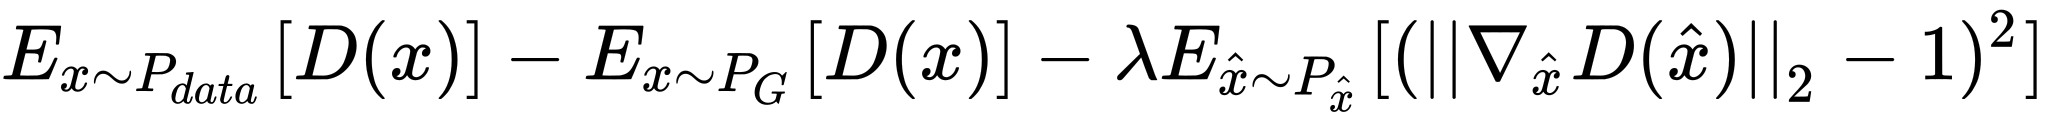
\includegraphics{pictures/wgan-gp.svg}

下面是WGAN-GP的具体代码实现,同WGAN,我们也只实现了他的训练代码,而模型我们直接使用DCGAN的模型.

    \begin{Verbatim}[commandchars=\\\{\}]
{\color{incolor}In [{\color{incolor}25}]:} \PY{k+kn}{import} \PY{n+nn}{torch}\PY{n+nn}{.}\PY{n+nn}{autograd} \PY{k}{as} \PY{n+nn}{autograd}
         
         \PY{k}{def} \PY{n+nf}{wgan\PYZus{}gp\PYZus{}train}\PY{p}{(}\PY{n}{trainloader}\PY{p}{,} \PY{n}{G}\PY{p}{,} \PY{n}{D}\PY{p}{,} \PY{n}{G\PYZus{}optimizer}\PY{p}{,} \PY{n}{D\PYZus{}optimizer}\PY{p}{,} \PY{n}{device}\PY{p}{,} \PY{n}{z\PYZus{}dim}\PY{p}{,} \PY{n}{lambda\PYZus{}}\PY{o}{=}\PY{l+m+mi}{10}\PY{p}{,} \PY{n}{n\PYZus{}d}\PY{o}{=}\PY{l+m+mi}{2}\PY{p}{)}\PY{p}{:}
             
             \PY{n}{D}\PY{o}{.}\PY{n}{train}\PY{p}{(}\PY{p}{)}
             \PY{n}{G}\PY{o}{.}\PY{n}{train}\PY{p}{(}\PY{p}{)}
             
             \PY{n}{D\PYZus{}total\PYZus{}loss} \PY{o}{=} \PY{l+m+mi}{0}
             \PY{n}{G\PYZus{}total\PYZus{}loss} \PY{o}{=} \PY{l+m+mi}{0}
             
             
             \PY{k}{for} \PY{n}{i}\PY{p}{,} \PY{p}{(}\PY{n}{x}\PY{p}{,} \PY{n}{\PYZus{}}\PY{p}{)} \PY{o+ow}{in} \PY{n+nb}{enumerate}\PY{p}{(}\PY{n}{trainloader}\PY{p}{)}\PY{p}{:}
                 \PY{n}{x} \PY{o}{=} \PY{n}{x}\PY{o}{.}\PY{n}{to}\PY{p}{(}\PY{n}{device}\PY{p}{)}
         
                 \PY{c+c1}{\PYZsh{} update D network}
                 \PY{c+c1}{\PYZsh{} D optimizer zero grads}
                 \PY{n}{D\PYZus{}optimizer}\PY{o}{.}\PY{n}{zero\PYZus{}grad}\PY{p}{(}\PY{p}{)}
                 
                 \PY{c+c1}{\PYZsh{} D real loss from real images}
                 \PY{n}{d\PYZus{}real} \PY{o}{=} \PY{n}{D}\PY{p}{(}\PY{n}{x}\PY{p}{)}
                 \PY{n}{d\PYZus{}real\PYZus{}loss} \PY{o}{=} \PY{o}{\PYZhy{}} \PY{n}{d\PYZus{}real}\PY{o}{.}\PY{n}{mean}\PY{p}{(}\PY{p}{)}
                 
                 \PY{c+c1}{\PYZsh{} D fake loss from fake images generated by G}
                 \PY{n}{z} \PY{o}{=} \PY{n}{torch}\PY{o}{.}\PY{n}{rand}\PY{p}{(}\PY{n}{x}\PY{o}{.}\PY{n}{size}\PY{p}{(}\PY{l+m+mi}{0}\PY{p}{)}\PY{p}{,} \PY{n}{z\PYZus{}dim}\PY{p}{)}\PY{o}{.}\PY{n}{to}\PY{p}{(}\PY{n}{device}\PY{p}{)}
                 \PY{n}{g\PYZus{}z} \PY{o}{=} \PY{n}{G}\PY{p}{(}\PY{n}{z}\PY{p}{)}
                 \PY{n}{d\PYZus{}fake} \PY{o}{=} \PY{n}{D}\PY{p}{(}\PY{n}{g\PYZus{}z}\PY{p}{)}
                 \PY{n}{d\PYZus{}fake\PYZus{}loss} \PY{o}{=} \PY{n}{d\PYZus{}fake}\PY{o}{.}\PY{n}{mean}\PY{p}{(}\PY{p}{)}
                 
                 \PY{c+c1}{\PYZsh{} D gradient penalty}
                 
                 \PY{c+c1}{\PYZsh{}   a random number epsilon}
                 \PY{n}{epsilon} \PY{o}{=} \PY{n}{torch}\PY{o}{.}\PY{n}{rand}\PY{p}{(}\PY{n}{x}\PY{o}{.}\PY{n}{size}\PY{p}{(}\PY{l+m+mi}{0}\PY{p}{)}\PY{p}{,} \PY{l+m+mi}{1}\PY{p}{,} \PY{l+m+mi}{1}\PY{p}{,} \PY{l+m+mi}{1}\PY{p}{)}\PY{o}{.}\PY{n}{cuda}\PY{p}{(}\PY{p}{)}
                 \PY{n}{x\PYZus{}hat} \PY{o}{=} \PY{n}{epsilon} \PY{o}{*} \PY{n}{x} \PY{o}{+} \PY{p}{(}\PY{l+m+mi}{1} \PY{o}{\PYZhy{}} \PY{n}{epsilon}\PY{p}{)} \PY{o}{*} \PY{n}{g\PYZus{}z}
                 \PY{n}{x\PYZus{}hat}\PY{o}{.}\PY{n}{requires\PYZus{}grad\PYZus{}}\PY{p}{(}\PY{k+kc}{True}\PY{p}{)}
         
                 \PY{n}{y\PYZus{}hat} \PY{o}{=} \PY{n}{D}\PY{p}{(}\PY{n}{x\PYZus{}hat}\PY{p}{)}
                 \PY{c+c1}{\PYZsh{}   computes the sum of gradients of y\PYZus{}hat with regard to x\PYZus{}hat}
                 \PY{n}{gradients} \PY{o}{=} \PY{n}{autograd}\PY{o}{.}\PY{n}{grad}\PY{p}{(}\PY{n}{outputs}\PY{o}{=}\PY{n}{y\PYZus{}hat}\PY{p}{,} \PY{n}{inputs}\PY{o}{=}\PY{n}{x\PYZus{}hat}\PY{p}{,} \PY{n}{grad\PYZus{}outputs}\PY{o}{=}\PY{n}{torch}\PY{o}{.}\PY{n}{ones}\PY{p}{(}\PY{n}{y\PYZus{}hat}\PY{o}{.}\PY{n}{size}\PY{p}{(}\PY{p}{)}\PY{p}{)}\PY{o}{.}\PY{n}{cuda}\PY{p}{(}\PY{p}{)}\PY{p}{,}
                                           \PY{n}{create\PYZus{}graph}\PY{o}{=}\PY{k+kc}{True}\PY{p}{,} \PY{n}{retain\PYZus{}graph}\PY{o}{=}\PY{k+kc}{True}\PY{p}{,} \PY{n}{only\PYZus{}inputs}\PY{o}{=}\PY{k+kc}{True}\PY{p}{)}\PY{p}{[}\PY{l+m+mi}{0}\PY{p}{]}
                 \PY{c+c1}{\PYZsh{}   computes gradientpenalty}
                 \PY{n}{gradient\PYZus{}penalty} \PY{o}{=}  \PY{n}{torch}\PY{o}{.}\PY{n}{mean}\PY{p}{(}\PY{p}{(}\PY{n}{gradients}\PY{o}{.}\PY{n}{view}\PY{p}{(}\PY{n}{gradients}\PY{o}{.}\PY{n}{size}\PY{p}{(}\PY{p}{)}\PY{p}{[}\PY{l+m+mi}{0}\PY{p}{]}\PY{p}{,} \PY{o}{\PYZhy{}}\PY{l+m+mi}{1}\PY{p}{)}\PY{o}{.}\PY{n}{norm}\PY{p}{(}\PY{n}{p}\PY{o}{=}\PY{l+m+mi}{2}\PY{p}{,} \PY{n}{dim}\PY{o}{=}\PY{l+m+mi}{1}\PY{p}{)} \PY{o}{\PYZhy{}} \PY{l+m+mi}{1}\PY{p}{)} \PY{o}{*}\PY{o}{*} \PY{l+m+mi}{2}\PY{p}{)}
                 
                 \PY{c+c1}{\PYZsh{} D backward and step}
                 \PY{n}{d\PYZus{}loss} \PY{o}{=} \PY{n}{d\PYZus{}real\PYZus{}loss} \PY{o}{+} \PY{n}{d\PYZus{}fake\PYZus{}loss} \PY{o}{+} \PY{n}{lambda\PYZus{}} \PY{o}{*} \PY{n}{gradient\PYZus{}penalty}
                 \PY{n}{d\PYZus{}loss}\PY{o}{.}\PY{n}{backward}\PY{p}{(}\PY{p}{)}
                 \PY{n}{D\PYZus{}optimizer}\PY{o}{.}\PY{n}{step}\PY{p}{(}\PY{p}{)}
                 
                     
                 \PY{n}{D\PYZus{}total\PYZus{}loss} \PY{o}{+}\PY{o}{=} \PY{n}{d\PYZus{}loss}\PY{o}{.}\PY{n}{item}\PY{p}{(}\PY{p}{)}
         
                 \PY{c+c1}{\PYZsh{} update G network}
                 \PY{c+c1}{\PYZsh{} G optimizer zero grads}
                 \PY{k}{if} \PY{p}{(}\PY{n}{i} \PY{o}{+} \PY{l+m+mi}{1}\PY{p}{)} \PY{o}{\PYZpc{}} \PY{n}{n\PYZus{}d} \PY{o}{==} \PY{l+m+mi}{0}\PY{p}{:}
                     \PY{n}{G\PYZus{}optimizer}\PY{o}{.}\PY{n}{zero\PYZus{}grad}\PY{p}{(}\PY{p}{)}
         
                     \PY{c+c1}{\PYZsh{} G loss}
                     \PY{n}{g\PYZus{}z} \PY{o}{=} \PY{n}{G}\PY{p}{(}\PY{n}{z}\PY{p}{)}
                     \PY{n}{d\PYZus{}fake} \PY{o}{=} \PY{n}{D}\PY{p}{(}\PY{n}{g\PYZus{}z}\PY{p}{)}
                     \PY{n}{g\PYZus{}loss} \PY{o}{=} \PY{o}{\PYZhy{}} \PY{n}{d\PYZus{}fake}\PY{o}{.}\PY{n}{mean}\PY{p}{(}\PY{p}{)}
         
                     \PY{c+c1}{\PYZsh{} G backward and step}
                     \PY{n}{g\PYZus{}loss}\PY{o}{.}\PY{n}{backward}\PY{p}{(}\PY{p}{)}
                     \PY{n}{G\PYZus{}optimizer}\PY{o}{.}\PY{n}{step}\PY{p}{(}\PY{p}{)}
                     
                     \PY{n}{G\PYZus{}total\PYZus{}loss} \PY{o}{+}\PY{o}{=} \PY{n}{g\PYZus{}loss}\PY{o}{.}\PY{n}{item}\PY{p}{(}\PY{p}{)}
             
             \PY{k}{return} \PY{n}{D\PYZus{}total\PYZus{}loss} \PY{o}{/} \PY{n+nb}{len}\PY{p}{(}\PY{n}{trainloader}\PY{p}{)}\PY{p}{,} \PY{n}{G\PYZus{}total\PYZus{}loss} \PY{o}{*} \PY{n}{n\PYZus{}d} \PY{o}{/} \PY{n+nb}{len}\PY{p}{(}\PY{n}{trainloader}\PY{p}{)}
\end{Verbatim}


    \begin{Verbatim}[commandchars=\\\{\}]
{\color{incolor}In [{\color{incolor}26}]:} \PY{c+c1}{\PYZsh{} hyper params}
         
         \PY{c+c1}{\PYZsh{} z dim}
         \PY{n}{latent\PYZus{}dim} \PY{o}{=} \PY{l+m+mi}{100}
         
         \PY{c+c1}{\PYZsh{} image size and channel}
         \PY{n}{image\PYZus{}size}\PY{o}{=}\PY{l+m+mi}{32}
         \PY{n}{image\PYZus{}channel}\PY{o}{=}\PY{l+m+mi}{3}
         
         \PY{c+c1}{\PYZsh{} Adam lr and betas}
         \PY{n}{learning\PYZus{}rate} \PY{o}{=} \PY{l+m+mf}{0.0002}
         \PY{n}{betas} \PY{o}{=} \PY{p}{(}\PY{l+m+mf}{0.5}\PY{p}{,} \PY{l+m+mf}{0.999}\PY{p}{)}
         
         \PY{c+c1}{\PYZsh{} epochs and batch size}
         \PY{n}{n\PYZus{}epochs} \PY{o}{=} \PY{l+m+mi}{300}
         \PY{n}{batch\PYZus{}size} \PY{o}{=} \PY{l+m+mi}{32}
         
         \PY{c+c1}{\PYZsh{} device : cpu or cuda:0/1/2/3}
         \PY{n}{device} \PY{o}{=} \PY{n}{torch}\PY{o}{.}\PY{n}{device}\PY{p}{(}\PY{l+s+s1}{\PYZsq{}}\PY{l+s+s1}{cuda:0}\PY{l+s+s1}{\PYZsq{}}\PY{p}{)}
         
         \PY{c+c1}{\PYZsh{} n\PYZus{}d: train D}
         \PY{n}{n\PYZus{}d} \PY{o}{=} \PY{l+m+mi}{2}
         \PY{n}{lambda\PYZus{}} \PY{o}{=} \PY{l+m+mi}{10}
         
         \PY{c+c1}{\PYZsh{} mnist dataset and dataloader}
         \PY{n}{train\PYZus{}dataset} \PY{o}{=} \PY{n}{load\PYZus{}furniture\PYZus{}data}\PY{p}{(}\PY{p}{)}
         \PY{n}{trainloader} \PY{o}{=} \PY{n}{torch}\PY{o}{.}\PY{n}{utils}\PY{o}{.}\PY{n}{data}\PY{o}{.}\PY{n}{DataLoader}\PY{p}{(}\PY{n}{train\PYZus{}dataset}\PY{p}{,} \PY{n}{batch\PYZus{}size}\PY{o}{=}\PY{n}{batch\PYZus{}size}\PY{p}{,} \PY{n}{shuffle}\PY{o}{=}\PY{k+kc}{True}\PY{p}{)}
         
         \PY{c+c1}{\PYZsh{} G and D model, use DCGAN, note that sigmoid is removed in D}
         \PY{n}{G} \PY{o}{=} \PY{n}{DCGenerator}\PY{p}{(}\PY{n}{image\PYZus{}size}\PY{o}{=}\PY{n}{image\PYZus{}size}\PY{p}{,} \PY{n}{latent\PYZus{}dim}\PY{o}{=}\PY{n}{latent\PYZus{}dim}\PY{p}{,} \PY{n}{output\PYZus{}channel}\PY{o}{=}\PY{n}{image\PYZus{}channel}\PY{p}{)}\PY{o}{.}\PY{n}{to}\PY{p}{(}\PY{n}{device}\PY{p}{)}
         \PY{n}{D} \PY{o}{=} \PY{n}{DCDiscriminator}\PY{p}{(}\PY{n}{image\PYZus{}size}\PY{o}{=}\PY{n}{image\PYZus{}size}\PY{p}{,} \PY{n}{input\PYZus{}channel}\PY{o}{=}\PY{n}{image\PYZus{}channel}\PY{p}{,} \PY{n}{sigmoid}\PY{o}{=}\PY{k+kc}{False}\PY{p}{)}\PY{o}{.}\PY{n}{to}\PY{p}{(}\PY{n}{device}\PY{p}{)}
         
         \PY{c+c1}{\PYZsh{} G and D optimizer, use Adam or SGD}
         \PY{n}{G\PYZus{}optimizer} \PY{o}{=} \PY{n}{optim}\PY{o}{.}\PY{n}{Adam}\PY{p}{(}\PY{n}{G}\PY{o}{.}\PY{n}{parameters}\PY{p}{(}\PY{p}{)}\PY{p}{,} \PY{n}{lr}\PY{o}{=}\PY{n}{learning\PYZus{}rate}\PY{p}{,} \PY{n}{betas}\PY{o}{=}\PY{n}{betas}\PY{p}{)}
         \PY{n}{D\PYZus{}optimizer} \PY{o}{=} \PY{n}{optim}\PY{o}{.}\PY{n}{Adam}\PY{p}{(}\PY{n}{D}\PY{o}{.}\PY{n}{parameters}\PY{p}{(}\PY{p}{)}\PY{p}{,} \PY{n}{lr}\PY{o}{=}\PY{n}{learning\PYZus{}rate}\PY{p}{,} \PY{n}{betas}\PY{o}{=}\PY{n}{betas}\PY{p}{)}
         
         \PY{n}{d\PYZus{}loss\PYZus{}hist} \PY{o}{=} \PY{p}{[}\PY{p}{]}
         \PY{n}{g\PYZus{}loss\PYZus{}hist} \PY{o}{=} \PY{p}{[}\PY{p}{]}
         
         \PY{k}{for} \PY{n}{epoch} \PY{o+ow}{in} \PY{n+nb}{range}\PY{p}{(}\PY{n}{n\PYZus{}epochs}\PY{p}{)}\PY{p}{:}
             \PY{n}{d\PYZus{}loss}\PY{p}{,} \PY{n}{g\PYZus{}loss} \PY{o}{=} \PY{n}{wgan\PYZus{}gp\PYZus{}train}\PY{p}{(}\PY{n}{trainloader}\PY{p}{,} \PY{n}{G}\PY{p}{,} \PY{n}{D}\PY{p}{,} \PY{n}{G\PYZus{}optimizer}\PY{p}{,} \PY{n}{D\PYZus{}optimizer}\PY{p}{,} \PY{n}{device}\PY{p}{,} 
                                    \PY{n}{z\PYZus{}dim}\PY{o}{=}\PY{n}{latent\PYZus{}dim}\PY{p}{,} \PY{n}{lambda\PYZus{}}\PY{o}{=}\PY{n}{lambda\PYZus{}}\PY{p}{,} \PY{n}{n\PYZus{}d}\PY{o}{=}\PY{n}{n\PYZus{}d}\PY{p}{)}
             \PY{n+nb}{print}\PY{p}{(}\PY{l+s+s1}{\PYZsq{}}\PY{l+s+s1}{Epoch }\PY{l+s+si}{\PYZob{}\PYZcb{}}\PY{l+s+s1}{: Train D loss: }\PY{l+s+si}{\PYZob{}:.4f\PYZcb{}}\PY{l+s+s1}{, G loss: }\PY{l+s+si}{\PYZob{}:.4f\PYZcb{}}\PY{l+s+s1}{\PYZsq{}}\PY{o}{.}\PY{n}{format}\PY{p}{(}\PY{n}{epoch}\PY{p}{,} \PY{n}{d\PYZus{}loss}\PY{p}{,} \PY{n}{g\PYZus{}loss}\PY{p}{)}\PY{p}{)}
             
             \PY{n}{d\PYZus{}loss\PYZus{}hist}\PY{o}{.}\PY{n}{append}\PY{p}{(}\PY{n}{d\PYZus{}loss}\PY{p}{)}
             \PY{n}{g\PYZus{}loss\PYZus{}hist}\PY{o}{.}\PY{n}{append}\PY{p}{(}\PY{n}{g\PYZus{}loss}\PY{p}{)}
             
             \PY{k}{if} \PY{n}{epoch} \PY{o}{==} \PY{l+m+mi}{0} \PY{o+ow}{or} \PY{p}{(}\PY{n}{epoch} \PY{o}{+} \PY{l+m+mi}{1}\PY{p}{)} \PY{o}{\PYZpc{}} \PY{l+m+mi}{10} \PY{o}{==} \PY{l+m+mi}{0}\PY{p}{:}
                 \PY{n}{visualize\PYZus{}results}\PY{p}{(}\PY{n}{G}\PY{p}{,} \PY{n}{device}\PY{p}{,} \PY{n}{latent\PYZus{}dim}\PY{p}{)}
\end{Verbatim}


    \begin{Verbatim}[commandchars=\\\{\}]
Epoch 0: Train D loss: 1.9138, G loss: 2.8894

    \end{Verbatim}

    \begin{center}
    \adjustimage{max size={0.9\linewidth}{0.9\paperheight}}{output_60_1.png}
    \end{center}
    { \hspace*{\fill} \\}
    
    \begin{Verbatim}[commandchars=\\\{\}]
Epoch 1: Train D loss: -7.6802, G loss: 7.2469
Epoch 2: Train D loss: -13.9764, G loss: 15.5410
Epoch 3: Train D loss: -21.0135, G loss: 22.7550
Epoch 4: Train D loss: -23.2528, G loss: 24.2562
Epoch 5: Train D loss: -20.1072, G loss: 20.7516
Epoch 6: Train D loss: -15.2331, G loss: 18.3803
Epoch 7: Train D loss: -14.9226, G loss: 19.0043
Epoch 8: Train D loss: -14.0151, G loss: 19.7235
Epoch 9: Train D loss: -13.1958, G loss: 19.7429

    \end{Verbatim}

    \begin{center}
    \adjustimage{max size={0.9\linewidth}{0.9\paperheight}}{output_60_3.png}
    \end{center}
    { \hspace*{\fill} \\}
    
    \begin{Verbatim}[commandchars=\\\{\}]
Epoch 10: Train D loss: -12.4196, G loss: 20.9996
Epoch 11: Train D loss: -11.9206, G loss: 20.4730
Epoch 12: Train D loss: -12.2786, G loss: 21.2064
Epoch 13: Train D loss: -11.7066, G loss: 21.5907
Epoch 14: Train D loss: -12.2409, G loss: 21.3554
Epoch 15: Train D loss: -12.3052, G loss: 21.6448
Epoch 16: Train D loss: -12.2074, G loss: 22.7216
Epoch 17: Train D loss: -12.2377, G loss: 22.9396
Epoch 18: Train D loss: -11.6817, G loss: 22.9095
Epoch 19: Train D loss: -12.2976, G loss: 23.5709

    \end{Verbatim}

    \begin{center}
    \adjustimage{max size={0.9\linewidth}{0.9\paperheight}}{output_60_5.png}
    \end{center}
    { \hspace*{\fill} \\}
    
    \begin{Verbatim}[commandchars=\\\{\}]
Epoch 20: Train D loss: -10.9933, G loss: 23.0542
Epoch 21: Train D loss: -10.8026, G loss: 23.7914
Epoch 22: Train D loss: -10.5049, G loss: 23.0612
Epoch 23: Train D loss: -11.1378, G loss: 24.1752
Epoch 24: Train D loss: -9.9463, G loss: 24.2370
Epoch 25: Train D loss: -11.3475, G loss: 25.0065
Epoch 26: Train D loss: -11.0203, G loss: 25.6521
Epoch 27: Train D loss: -10.3455, G loss: 25.9421
Epoch 28: Train D loss: -9.9056, G loss: 25.7743
Epoch 29: Train D loss: -6.2187, G loss: 25.8360

    \end{Verbatim}

    \begin{center}
    \adjustimage{max size={0.9\linewidth}{0.9\paperheight}}{output_60_7.png}
    \end{center}
    { \hspace*{\fill} \\}
    
    \begin{Verbatim}[commandchars=\\\{\}]
Epoch 30: Train D loss: -10.1146, G loss: 27.3913
Epoch 31: Train D loss: -10.2916, G loss: 25.4187
Epoch 32: Train D loss: -11.0253, G loss: 26.7513
Epoch 33: Train D loss: -10.5094, G loss: 26.8595
Epoch 34: Train D loss: -9.3126, G loss: 26.1853
Epoch 35: Train D loss: -8.3496, G loss: 27.7662
Epoch 36: Train D loss: -7.3177, G loss: 28.9023
Epoch 37: Train D loss: -9.7651, G loss: 28.3674
Epoch 38: Train D loss: -9.0622, G loss: 29.1948
Epoch 39: Train D loss: -9.8254, G loss: 28.3662

    \end{Verbatim}

    \begin{center}
    \adjustimage{max size={0.9\linewidth}{0.9\paperheight}}{output_60_9.png}
    \end{center}
    { \hspace*{\fill} \\}
    
    \begin{Verbatim}[commandchars=\\\{\}]
Epoch 40: Train D loss: -8.9681, G loss: 28.7342
Epoch 41: Train D loss: -8.8292, G loss: 28.3998
Epoch 42: Train D loss: -3.0938, G loss: 27.4003
Epoch 43: Train D loss: -7.0819, G loss: 31.2069
Epoch 44: Train D loss: -7.3786, G loss: 29.6973
Epoch 45: Train D loss: -7.9696, G loss: 28.7681
Epoch 46: Train D loss: -6.9240, G loss: 29.7559
Epoch 47: Train D loss: -7.1298, G loss: 29.6157
Epoch 48: Train D loss: -6.9581, G loss: 28.6319
Epoch 49: Train D loss: -6.5274, G loss: 28.4532

    \end{Verbatim}

    \begin{center}
    \adjustimage{max size={0.9\linewidth}{0.9\paperheight}}{output_60_11.png}
    \end{center}
    { \hspace*{\fill} \\}
    
    \begin{Verbatim}[commandchars=\\\{\}]
Epoch 50: Train D loss: -7.1294, G loss: 29.0073
Epoch 51: Train D loss: -6.7017, G loss: 28.6002
Epoch 52: Train D loss: -4.9460, G loss: 28.5490
Epoch 53: Train D loss: -4.9684, G loss: 27.5253
Epoch 54: Train D loss: -6.1524, G loss: 30.4332
Epoch 55: Train D loss: -6.0944, G loss: 28.4493
Epoch 56: Train D loss: -5.5228, G loss: 28.7265
Epoch 57: Train D loss: -6.3676, G loss: 30.5054
Epoch 58: Train D loss: -5.7836, G loss: 26.7295
Epoch 59: Train D loss: -6.8589, G loss: 29.0402

    \end{Verbatim}

    \begin{center}
    \adjustimage{max size={0.9\linewidth}{0.9\paperheight}}{output_60_13.png}
    \end{center}
    { \hspace*{\fill} \\}
    
    \begin{Verbatim}[commandchars=\\\{\}]
Epoch 60: Train D loss: -5.9558, G loss: 28.0232
Epoch 61: Train D loss: -5.1307, G loss: 29.9335
Epoch 62: Train D loss: -6.2894, G loss: 29.9679
Epoch 63: Train D loss: -5.8852, G loss: 26.5735
Epoch 64: Train D loss: -6.3535, G loss: 29.4922
Epoch 65: Train D loss: -4.8865, G loss: 26.5939
Epoch 66: Train D loss: -5.1508, G loss: 29.2366
Epoch 67: Train D loss: -5.8137, G loss: 28.8419
Epoch 68: Train D loss: -5.7358, G loss: 29.7355
Epoch 69: Train D loss: -5.6528, G loss: 28.0221

    \end{Verbatim}

    \begin{center}
    \adjustimage{max size={0.9\linewidth}{0.9\paperheight}}{output_60_15.png}
    \end{center}
    { \hspace*{\fill} \\}
    
    \begin{Verbatim}[commandchars=\\\{\}]
Epoch 70: Train D loss: -4.9963, G loss: 28.9994
Epoch 71: Train D loss: -5.8181, G loss: 29.4565
Epoch 72: Train D loss: -4.7978, G loss: 28.7896
Epoch 73: Train D loss: -5.9688, G loss: 31.9322
Epoch 74: Train D loss: -2.4451, G loss: 24.5670
Epoch 75: Train D loss: -1.8079, G loss: 27.6129
Epoch 76: Train D loss: -3.4372, G loss: 27.6535
Epoch 77: Train D loss: -4.1568, G loss: 30.3867
Epoch 78: Train D loss: -5.1961, G loss: 28.9180
Epoch 79: Train D loss: -5.4937, G loss: 32.1237

    \end{Verbatim}

    \begin{center}
    \adjustimage{max size={0.9\linewidth}{0.9\paperheight}}{output_60_17.png}
    \end{center}
    { \hspace*{\fill} \\}
    
    \begin{Verbatim}[commandchars=\\\{\}]
Epoch 80: Train D loss: -5.2063, G loss: 29.1556
Epoch 81: Train D loss: -5.7071, G loss: 31.8133
Epoch 82: Train D loss: -5.6945, G loss: 32.4153
Epoch 83: Train D loss: -6.0853, G loss: 30.1674
Epoch 84: Train D loss: -5.6299, G loss: 31.3750
Epoch 85: Train D loss: -6.0927, G loss: 32.5744
Epoch 86: Train D loss: -6.2900, G loss: 31.8117
Epoch 87: Train D loss: -5.7372, G loss: 32.8766
Epoch 88: Train D loss: -5.9741, G loss: 32.2264
Epoch 89: Train D loss: -6.3744, G loss: 33.0866

    \end{Verbatim}

    \begin{center}
    \adjustimage{max size={0.9\linewidth}{0.9\paperheight}}{output_60_19.png}
    \end{center}
    { \hspace*{\fill} \\}
    
    \begin{Verbatim}[commandchars=\\\{\}]
Epoch 90: Train D loss: -5.9845, G loss: 35.0445
Epoch 91: Train D loss: -3.8307, G loss: 29.5940
Epoch 92: Train D loss: -3.1370, G loss: 33.8698
Epoch 93: Train D loss: -5.9951, G loss: 31.5741
Epoch 94: Train D loss: -6.2503, G loss: 34.3288
Epoch 95: Train D loss: -6.4692, G loss: 32.2232
Epoch 96: Train D loss: -5.6636, G loss: 31.4132
Epoch 97: Train D loss: -6.1194, G loss: 33.9555
Epoch 98: Train D loss: -6.3148, G loss: 34.0157
Epoch 99: Train D loss: -6.2206, G loss: 31.9390

    \end{Verbatim}

    \begin{center}
    \adjustimage{max size={0.9\linewidth}{0.9\paperheight}}{output_60_21.png}
    \end{center}
    { \hspace*{\fill} \\}
    
    \begin{Verbatim}[commandchars=\\\{\}]
Epoch 100: Train D loss: -6.3356, G loss: 35.0574
Epoch 101: Train D loss: -6.0658, G loss: 33.4022
Epoch 102: Train D loss: -6.4971, G loss: 33.7549
Epoch 103: Train D loss: -6.8912, G loss: 32.8541
Epoch 104: Train D loss: -6.7471, G loss: 34.5419
Epoch 105: Train D loss: -6.6885, G loss: 35.3761
Epoch 106: Train D loss: -5.6554, G loss: 30.6172
Epoch 107: Train D loss: -6.3271, G loss: 35.7289
Epoch 108: Train D loss: -7.2940, G loss: 33.4487
Epoch 109: Train D loss: -6.8586, G loss: 34.7442

    \end{Verbatim}

    \begin{center}
    \adjustimage{max size={0.9\linewidth}{0.9\paperheight}}{output_60_23.png}
    \end{center}
    { \hspace*{\fill} \\}
    
    \begin{Verbatim}[commandchars=\\\{\}]
Epoch 110: Train D loss: -7.2201, G loss: 33.2813
Epoch 111: Train D loss: -4.6217, G loss: 31.8885
Epoch 112: Train D loss: -0.8692, G loss: 30.7615
Epoch 113: Train D loss: -0.4826, G loss: 27.9577
Epoch 114: Train D loss: -1.5283, G loss: 31.1836
Epoch 115: Train D loss: -1.5166, G loss: 29.5327
Epoch 116: Train D loss: -2.2398, G loss: 31.7592
Epoch 117: Train D loss: -2.3865, G loss: 32.6728
Epoch 118: Train D loss: -3.0378, G loss: 31.9959
Epoch 119: Train D loss: -3.2661, G loss: 34.9607

    \end{Verbatim}

    \begin{center}
    \adjustimage{max size={0.9\linewidth}{0.9\paperheight}}{output_60_25.png}
    \end{center}
    { \hspace*{\fill} \\}
    
    \begin{Verbatim}[commandchars=\\\{\}]
Epoch 120: Train D loss: -4.0260, G loss: 36.1813
Epoch 121: Train D loss: -4.0354, G loss: 34.1318
Epoch 122: Train D loss: -4.2423, G loss: 34.6511
Epoch 123: Train D loss: -4.4612, G loss: 35.7181
Epoch 124: Train D loss: -4.7373, G loss: 35.2861
Epoch 125: Train D loss: -5.1802, G loss: 37.3874
Epoch 126: Train D loss: -4.9474, G loss: 35.3122
Epoch 127: Train D loss: -5.0750, G loss: 37.3254
Epoch 128: Train D loss: -5.6584, G loss: 37.2527
Epoch 129: Train D loss: -5.2755, G loss: 36.7940

    \end{Verbatim}

    \begin{center}
    \adjustimage{max size={0.9\linewidth}{0.9\paperheight}}{output_60_27.png}
    \end{center}
    { \hspace*{\fill} \\}
    
    \begin{Verbatim}[commandchars=\\\{\}]
Epoch 130: Train D loss: -5.6698, G loss: 37.5867
Epoch 131: Train D loss: -5.6408, G loss: 37.5685
Epoch 132: Train D loss: -5.6809, G loss: 38.6829
Epoch 133: Train D loss: -6.4214, G loss: 37.7465
Epoch 134: Train D loss: -5.4657, G loss: 40.0482
Epoch 135: Train D loss: -6.2278, G loss: 39.2800
Epoch 136: Train D loss: -6.5424, G loss: 41.0994
Epoch 137: Train D loss: -5.8239, G loss: 36.7432
Epoch 138: Train D loss: -5.8030, G loss: 38.9744
Epoch 139: Train D loss: -6.2140, G loss: 41.0691

    \end{Verbatim}

    \begin{center}
    \adjustimage{max size={0.9\linewidth}{0.9\paperheight}}{output_60_29.png}
    \end{center}
    { \hspace*{\fill} \\}
    
    \begin{Verbatim}[commandchars=\\\{\}]
Epoch 140: Train D loss: -6.1770, G loss: 39.9699
Epoch 141: Train D loss: -6.4609, G loss: 40.9406
Epoch 142: Train D loss: -6.2624, G loss: 39.3125
Epoch 143: Train D loss: -5.4924, G loss: 41.5853
Epoch 144: Train D loss: -4.9029, G loss: 38.6706
Epoch 145: Train D loss: -5.4920, G loss: 41.1641
Epoch 146: Train D loss: -6.0588, G loss: 40.2789
Epoch 147: Train D loss: -6.1547, G loss: 40.2177
Epoch 148: Train D loss: -6.2908, G loss: 39.7714
Epoch 149: Train D loss: -6.5084, G loss: 41.0793

    \end{Verbatim}

    \begin{center}
    \adjustimage{max size={0.9\linewidth}{0.9\paperheight}}{output_60_31.png}
    \end{center}
    { \hspace*{\fill} \\}
    
    \begin{Verbatim}[commandchars=\\\{\}]
Epoch 150: Train D loss: -4.3467, G loss: 40.4254
Epoch 151: Train D loss: -5.4771, G loss: 39.4178
Epoch 152: Train D loss: -6.3703, G loss: 40.7262
Epoch 153: Train D loss: -6.4533, G loss: 41.9639
Epoch 154: Train D loss: -6.3656, G loss: 40.1785
Epoch 155: Train D loss: -4.6848, G loss: 40.5686
Epoch 156: Train D loss: -1.2672, G loss: 36.0871
Epoch 157: Train D loss: -3.1198, G loss: 38.5695
Epoch 158: Train D loss: -4.1636, G loss: 41.8224
Epoch 159: Train D loss: -5.1912, G loss: 40.9218

    \end{Verbatim}

    \begin{center}
    \adjustimage{max size={0.9\linewidth}{0.9\paperheight}}{output_60_33.png}
    \end{center}
    { \hspace*{\fill} \\}
    
    \begin{Verbatim}[commandchars=\\\{\}]
Epoch 160: Train D loss: -4.9568, G loss: 41.7201
Epoch 161: Train D loss: -6.1029, G loss: 42.7636
Epoch 162: Train D loss: -5.7253, G loss: 40.2004
Epoch 163: Train D loss: -6.2200, G loss: 42.4481
Epoch 164: Train D loss: -5.4720, G loss: 42.9697
Epoch 165: Train D loss: -5.8613, G loss: 42.9216
Epoch 166: Train D loss: -5.9695, G loss: 41.4727
Epoch 167: Train D loss: -5.2325, G loss: 43.0106
Epoch 168: Train D loss: -5.9471, G loss: 43.8186
Epoch 169: Train D loss: -5.8720, G loss: 41.6714

    \end{Verbatim}

    \begin{center}
    \adjustimage{max size={0.9\linewidth}{0.9\paperheight}}{output_60_35.png}
    \end{center}
    { \hspace*{\fill} \\}
    
    \begin{Verbatim}[commandchars=\\\{\}]
Epoch 170: Train D loss: -6.4582, G loss: 41.9953
Epoch 171: Train D loss: -5.4550, G loss: 44.9441
Epoch 172: Train D loss: -5.8557, G loss: 43.3123
Epoch 173: Train D loss: -5.9495, G loss: 41.2810
Epoch 174: Train D loss: -5.8638, G loss: 44.8705
Epoch 175: Train D loss: -5.0399, G loss: 40.8322
Epoch 176: Train D loss: -3.7404, G loss: 42.2024
Epoch 177: Train D loss: -5.3755, G loss: 43.2599
Epoch 178: Train D loss: -6.1208, G loss: 42.8078
Epoch 179: Train D loss: -6.6627, G loss: 43.2770

    \end{Verbatim}

    \begin{center}
    \adjustimage{max size={0.9\linewidth}{0.9\paperheight}}{output_60_37.png}
    \end{center}
    { \hspace*{\fill} \\}
    
    \begin{Verbatim}[commandchars=\\\{\}]
Epoch 180: Train D loss: -5.8691, G loss: 43.0672
Epoch 181: Train D loss: -1.8263, G loss: 37.1000
Epoch 182: Train D loss: -3.6349, G loss: 41.5021
Epoch 183: Train D loss: -6.0211, G loss: 44.2321
Epoch 184: Train D loss: -6.2053, G loss: 40.3498
Epoch 185: Train D loss: -6.3287, G loss: 44.4458
Epoch 186: Train D loss: -6.1770, G loss: 44.2348
Epoch 187: Train D loss: -6.5091, G loss: 43.5525
Epoch 188: Train D loss: -5.8698, G loss: 43.2526
Epoch 189: Train D loss: -3.1748, G loss: 41.6122

    \end{Verbatim}

    \begin{center}
    \adjustimage{max size={0.9\linewidth}{0.9\paperheight}}{output_60_39.png}
    \end{center}
    { \hspace*{\fill} \\}
    
    \begin{Verbatim}[commandchars=\\\{\}]
Epoch 190: Train D loss: -0.8596, G loss: 40.9880
Epoch 191: Train D loss: -1.2718, G loss: 39.4914
Epoch 192: Train D loss: -1.7716, G loss: 41.7897
Epoch 193: Train D loss: -2.1584, G loss: 42.0713
Epoch 194: Train D loss: -2.6079, G loss: 44.4238
Epoch 195: Train D loss: -3.0127, G loss: 43.3047
Epoch 196: Train D loss: -3.3802, G loss: 44.0216
Epoch 197: Train D loss: -3.5756, G loss: 45.7562
Epoch 198: Train D loss: -4.0073, G loss: 43.2747
Epoch 199: Train D loss: -4.4650, G loss: 46.8713

    \end{Verbatim}

    \begin{center}
    \adjustimage{max size={0.9\linewidth}{0.9\paperheight}}{output_60_41.png}
    \end{center}
    { \hspace*{\fill} \\}
    
    \begin{Verbatim}[commandchars=\\\{\}]
Epoch 200: Train D loss: -5.0532, G loss: 43.4768
Epoch 201: Train D loss: -4.6917, G loss: 47.4972
Epoch 202: Train D loss: -5.0556, G loss: 43.8115
Epoch 203: Train D loss: -5.3890, G loss: 46.5626
Epoch 204: Train D loss: -5.7181, G loss: 45.2515
Epoch 205: Train D loss: -5.2730, G loss: 46.3621
Epoch 206: Train D loss: -5.7230, G loss: 45.2541
Epoch 207: Train D loss: -4.8701, G loss: 46.7109
Epoch 208: Train D loss: -6.8482, G loss: 46.2462
Epoch 209: Train D loss: -6.0709, G loss: 46.9169

    \end{Verbatim}

    \begin{center}
    \adjustimage{max size={0.9\linewidth}{0.9\paperheight}}{output_60_43.png}
    \end{center}
    { \hspace*{\fill} \\}
    
    \begin{Verbatim}[commandchars=\\\{\}]
Epoch 210: Train D loss: -6.5905, G loss: 47.0285
Epoch 211: Train D loss: -3.0712, G loss: 43.3368
Epoch 212: Train D loss: -5.0670, G loss: 46.4584
Epoch 213: Train D loss: -6.3289, G loss: 47.0023
Epoch 214: Train D loss: -7.8861, G loss: 44.7275
Epoch 215: Train D loss: -4.9834, G loss: 48.9583
Epoch 216: Train D loss: -4.5199, G loss: 42.7631
Epoch 217: Train D loss: -6.2741, G loss: 46.9830
Epoch 218: Train D loss: -6.1742, G loss: 45.9001
Epoch 219: Train D loss: -6.4805, G loss: 47.3471

    \end{Verbatim}

    \begin{center}
    \adjustimage{max size={0.9\linewidth}{0.9\paperheight}}{output_60_45.png}
    \end{center}
    { \hspace*{\fill} \\}
    
    \begin{Verbatim}[commandchars=\\\{\}]
Epoch 220: Train D loss: -6.7768, G loss: 43.9809
Epoch 221: Train D loss: -3.9302, G loss: 47.4409
Epoch 222: Train D loss: -7.2204, G loss: 43.1501
Epoch 223: Train D loss: -6.2453, G loss: 48.5988
Epoch 224: Train D loss: -6.8884, G loss: 45.3312
Epoch 225: Train D loss: -6.2709, G loss: 45.0827
Epoch 226: Train D loss: -6.1376, G loss: 47.2810
Epoch 227: Train D loss: -6.3655, G loss: 46.9446
Epoch 228: Train D loss: -5.2184, G loss: 46.1632
Epoch 229: Train D loss: -5.6828, G loss: 41.6041

    \end{Verbatim}

    \begin{center}
    \adjustimage{max size={0.9\linewidth}{0.9\paperheight}}{output_60_47.png}
    \end{center}
    { \hspace*{\fill} \\}
    
    \begin{Verbatim}[commandchars=\\\{\}]
Epoch 230: Train D loss: -6.1699, G loss: 49.2187
Epoch 231: Train D loss: -7.3552, G loss: 46.4724
Epoch 232: Train D loss: -4.8275, G loss: 44.5619
Epoch 233: Train D loss: -0.2607, G loss: 40.7146
Epoch 234: Train D loss: -0.6105, G loss: 39.9514
Epoch 235: Train D loss: -1.7170, G loss: 41.9917
Epoch 236: Train D loss: -2.1563, G loss: 43.3827
Epoch 237: Train D loss: -2.2252, G loss: 42.5559
Epoch 238: Train D loss: -2.6369, G loss: 44.7550
Epoch 239: Train D loss: -3.2773, G loss: 44.3916

    \end{Verbatim}

    \begin{center}
    \adjustimage{max size={0.9\linewidth}{0.9\paperheight}}{output_60_49.png}
    \end{center}
    { \hspace*{\fill} \\}
    
    \begin{Verbatim}[commandchars=\\\{\}]
Epoch 240: Train D loss: -3.4813, G loss: 45.2458
Epoch 241: Train D loss: -3.5038, G loss: 45.8402
Epoch 242: Train D loss: -4.1712, G loss: 46.5760
Epoch 243: Train D loss: -4.4579, G loss: 47.2575
Epoch 244: Train D loss: -4.4962, G loss: 46.3450
Epoch 245: Train D loss: -4.9980, G loss: 47.6786
Epoch 246: Train D loss: -5.1048, G loss: 47.6894
Epoch 247: Train D loss: -5.3046, G loss: 48.6975
Epoch 248: Train D loss: -5.6280, G loss: 48.2731
Epoch 249: Train D loss: -5.7237, G loss: 49.1804

    \end{Verbatim}

    \begin{center}
    \adjustimage{max size={0.9\linewidth}{0.9\paperheight}}{output_60_51.png}
    \end{center}
    { \hspace*{\fill} \\}
    
    \begin{Verbatim}[commandchars=\\\{\}]
Epoch 250: Train D loss: -5.8676, G loss: 48.3169
Epoch 251: Train D loss: -6.0179, G loss: 48.5784
Epoch 252: Train D loss: -6.0945, G loss: 48.3256
Epoch 253: Train D loss: -6.1686, G loss: 48.9060
Epoch 254: Train D loss: -6.3298, G loss: 49.1026
Epoch 255: Train D loss: -6.1382, G loss: 47.5019
Epoch 256: Train D loss: -6.3900, G loss: 49.5991
Epoch 257: Train D loss: -6.1522, G loss: 48.0346
Epoch 258: Train D loss: -6.1350, G loss: 49.1006
Epoch 259: Train D loss: -4.7894, G loss: 48.0324

    \end{Verbatim}

    \begin{center}
    \adjustimage{max size={0.9\linewidth}{0.9\paperheight}}{output_60_53.png}
    \end{center}
    { \hspace*{\fill} \\}
    
    \begin{Verbatim}[commandchars=\\\{\}]
Epoch 260: Train D loss: -1.5837, G loss: 44.2659
Epoch 261: Train D loss: -2.3337, G loss: 44.7671
Epoch 262: Train D loss: -3.4709, G loss: 46.4892
Epoch 263: Train D loss: -4.1336, G loss: 48.1598
Epoch 264: Train D loss: -4.8502, G loss: 47.5502
Epoch 265: Train D loss: -5.2265, G loss: 49.3409
Epoch 266: Train D loss: -5.4116, G loss: 50.3503
Epoch 267: Train D loss: -6.0815, G loss: 49.6595
Epoch 268: Train D loss: -6.4849, G loss: 50.4343
Epoch 269: Train D loss: -6.5729, G loss: 52.4809

    \end{Verbatim}

    \begin{center}
    \adjustimage{max size={0.9\linewidth}{0.9\paperheight}}{output_60_55.png}
    \end{center}
    { \hspace*{\fill} \\}
    
    \begin{Verbatim}[commandchars=\\\{\}]
Epoch 270: Train D loss: -6.6392, G loss: 45.5516
Epoch 271: Train D loss: -6.4586, G loss: 53.0016
Epoch 272: Train D loss: -7.0740, G loss: 49.7016
Epoch 273: Train D loss: -6.7721, G loss: 51.8330
Epoch 274: Train D loss: -7.6541, G loss: 47.9551
Epoch 275: Train D loss: -6.3659, G loss: 52.8365
Epoch 276: Train D loss: -6.9196, G loss: 49.1662
Epoch 277: Train D loss: -7.1626, G loss: 50.2655
Epoch 278: Train D loss: -7.5302, G loss: 50.8964
Epoch 279: Train D loss: -6.3621, G loss: 49.4112

    \end{Verbatim}

    \begin{center}
    \adjustimage{max size={0.9\linewidth}{0.9\paperheight}}{output_60_57.png}
    \end{center}
    { \hspace*{\fill} \\}
    
    \begin{Verbatim}[commandchars=\\\{\}]
Epoch 280: Train D loss: -6.7418, G loss: 50.4388
Epoch 281: Train D loss: -7.4659, G loss: 51.7839
Epoch 282: Train D loss: -7.3289, G loss: 48.5114
Epoch 283: Train D loss: -5.4964, G loss: 51.1913
Epoch 284: Train D loss: -7.2117, G loss: 50.3560
Epoch 285: Train D loss: -7.2201, G loss: 51.5217
Epoch 286: Train D loss: -6.8211, G loss: 47.5604
Epoch 287: Train D loss: -6.7599, G loss: 51.5783
Epoch 288: Train D loss: -7.2045, G loss: 50.4178
Epoch 289: Train D loss: -0.8784, G loss: 46.7346

    \end{Verbatim}

    \begin{center}
    \adjustimage{max size={0.9\linewidth}{0.9\paperheight}}{output_60_59.png}
    \end{center}
    { \hspace*{\fill} \\}
    
    \begin{Verbatim}[commandchars=\\\{\}]
Epoch 290: Train D loss: -2.7672, G loss: 48.2613
Epoch 291: Train D loss: -4.2054, G loss: 49.7231
Epoch 292: Train D loss: -4.9421, G loss: 48.8620
Epoch 293: Train D loss: -5.5126, G loss: 50.3784
Epoch 294: Train D loss: -6.5394, G loss: 48.1095
Epoch 295: Train D loss: -6.0191, G loss: 51.5037
Epoch 296: Train D loss: -6.4718, G loss: 46.5220
Epoch 297: Train D loss: -6.8359, G loss: 51.0366
Epoch 298: Train D loss: -6.4938, G loss: 46.4618
Epoch 299: Train D loss: -7.6896, G loss: 46.7400

    \end{Verbatim}

    \begin{center}
    \adjustimage{max size={0.9\linewidth}{0.9\paperheight}}{output_60_61.png}
    \end{center}
    { \hspace*{\fill} \\}
    
    同理,观察loss曲线和D上的参数分布.

    \begin{Verbatim}[commandchars=\\\{\}]
{\color{incolor}In [{\color{incolor}27}]:} \PY{n}{loss\PYZus{}plot}\PY{p}{(}\PY{n}{d\PYZus{}loss\PYZus{}hist}\PY{p}{,} \PY{n}{g\PYZus{}loss\PYZus{}hist}\PY{p}{)}
\end{Verbatim}


    \begin{center}
    \adjustimage{max size={0.9\linewidth}{0.9\paperheight}}{output_62_0.png}
    \end{center}
    { \hspace*{\fill} \\}
    
    \begin{Verbatim}[commandchars=\\\{\}]
{\color{incolor}In [{\color{incolor}28}]:} \PY{n}{show\PYZus{}d\PYZus{}params}\PY{p}{(}\PY{n}{D}\PY{p}{)}
\end{Verbatim}


    \begin{center}
    \adjustimage{max size={0.9\linewidth}{0.9\paperheight}}{output_63_0.png}
    \end{center}
    { \hspace*{\fill} \\}
    
    \hypertarget{ux4f5cux4e1a}{%
\paragraph{\texorpdfstring{\textbf{作业}:}{作业:}}\label{ux4f5cux4e1a}}

观察WGAN和WGAN-GP生成器生成的图片效果,它们在相同epoch时生成的图片效果(或者说生成图片达到效果所需要epoch数量),它们的loss曲线以及D的参数分布,说说有什么不同?

    \textbf{答}:


    % Add a bibliography block to the postdoc
    
    
    
    \end{document}
